\documentclass[5p]{elsarticle}
%DIF LATEXDIFF DIFFERENCE FILE
%DIF DEL /home/anton/Desktop/SphereTDP/Latex/main.tex   Tue Jul 13 09:14:51 2021
%DIF ADD main.tex                                       Tue Jul 13 18:58:05 2021

\usepackage{lineno,hyperref}

%%%%%%%%%%%%%%%%%%%%%%%%%%%%%%%%%%%%%%%%%%%%%%%%%%%%%%%%%%
%% Packages and custom commands added by Authors %%%%%%%%%
%%%%%%%%%%%%%%%%%%%%%%%%%%%%%%%%%%%%%%%%%%%%%%%%%%%%%%%%%%
\usepackage{todonotes}
\usepackage{xifthen}
\usepackage{amsmath}
%DIF 11-12d11
%DIF < \usepackage{mathtools}
%DIF < \usepackage{breqn}
%DIF -------
\usepackage{siunitx}
\usepackage[ruled,vlined]{algorithm2e}

\renewcommand{\vec}[1]{\mathbf{#1}}

\def\block(#1,#2)#3{\multicolumn{#2}{c}{\multirow{#1}{*}{$ #3 $}}}

\newcommand{\norm}[2][]{%
\ifthenelse{\equal{#1}{}}{\left|\left| #2 \right|\right|}{\left|\left| #2 \right|\right|_{#1}}}
\newcommand{\pardiff}[1]{\frac{\partial}{\partial #1}}
\renewcommand{\epsilon}{\varepsilon}

\DeclareSIUnit\pts{points}

\renewcommand\floatpagefraction{1}
\renewcommand\topfraction{1}
\renewcommand\bottomfraction{1}
\renewcommand\textfraction{0}
%%%%%%%%%%%%%%%%%%%%%%%%%%%%%%%%%%%%%%%%%%%%%%%%%%%%%%%%%%

\modulolinenumbers[5]

\journal{IOJPRS}

%%%%%%%%%%%%%%%%%%%%%%%
%% Elsevier bibliography styles
%%%%%%%%%%%%%%%%%%%%%%%
%% To change the style, put a % in front of the second line of the current style and
%% remove the % from the second line of the style you would like to use.
%%%%%%%%%%%%%%%%%%%%%%%

%% Numberedss
%\bibliographystyle{model1-num-names}

%% Numbered without titlesbb
%\bibliographystyle{model1a-num-names}

%% Harvard
%\bibliographystyle{model2-names.bst}\biboptions{authoryear}

%% Vancouver numbered
%\usepackage{numcompress}\bibliographystyle{model3-num-names}

%% Vancouver name/year
%\usepackage{numcompress}\bibliographystyle{model4-names}\biboptions{authoryear}

%% APA style
%\bibliographystyle{model5-names}\biboptions{authoryear}

%% AMA style
%\usepackage{numcompress}\bibliographystyle{model6-num-names}

%% `Elsevier LaTeX' style
\bibliographystyle{elsarticle-num}
%%%%%%%%%%%%%%%%%%%%%%%
%DIF PREAMBLE EXTENSION ADDED BY LATEXDIFF
%DIF UNDERLINE PREAMBLE %DIF PREAMBLE
\RequirePackage[normalem]{ulem} %DIF PREAMBLE
\RequirePackage{color}\definecolor{RED}{rgb}{1,0,0}\definecolor{BLUE}{rgb}{0,0,1} %DIF PREAMBLE
\providecommand{\DIFaddtex}[1]{{\protect\color{blue}\uwave{#1}}} %DIF PREAMBLE
\providecommand{\DIFdeltex}[1]{{\protect\color{red}\sout{#1}}}                      %DIF PREAMBLE
%DIF SAFE PREAMBLE %DIF PREAMBLE
\providecommand{\DIFaddbegin}{} %DIF PREAMBLE
\providecommand{\DIFaddend}{} %DIF PREAMBLE
\providecommand{\DIFdelbegin}{} %DIF PREAMBLE
\providecommand{\DIFdelend}{} %DIF PREAMBLE
\providecommand{\DIFmodbegin}{} %DIF PREAMBLE
\providecommand{\DIFmodend}{} %DIF PREAMBLE
%DIF FLOATSAFE PREAMBLE %DIF PREAMBLE
\providecommand{\DIFaddFL}[1]{\DIFadd{#1}} %DIF PREAMBLE
\providecommand{\DIFdelFL}[1]{\DIFdel{#1}} %DIF PREAMBLE
\providecommand{\DIFaddbeginFL}{} %DIF PREAMBLE
\providecommand{\DIFaddendFL}{} %DIF PREAMBLE
\providecommand{\DIFdelbeginFL}{} %DIF PREAMBLE
\providecommand{\DIFdelendFL}{} %DIF PREAMBLE
%DIF HYPERREF PREAMBLE %DIF PREAMBLE
\providecommand{\DIFadd}[1]{\texorpdfstring{\DIFaddtex{#1}}{#1}} %DIF PREAMBLE
\providecommand{\DIFdel}[1]{\texorpdfstring{\DIFdeltex{#1}}{}} %DIF PREAMBLE
%DIF LISTINGS PREAMBLE %DIF PREAMBLE
\RequirePackage{listings} %DIF PREAMBLE
\RequirePackage{color} %DIF PREAMBLE
\lstdefinelanguage{DIFcode}{ %DIF PREAMBLE
%DIF DIFCODE_UNDERLINE %DIF PREAMBLE
  moredelim=[il][\color{red}\sout]{\%DIF\ <\ }, %DIF PREAMBLE
  moredelim=[il][\color{blue}\uwave]{\%DIF\ >\ } %DIF PREAMBLE
} %DIF PREAMBLE
\lstdefinestyle{DIFverbatimstyle}{ %DIF PREAMBLE
	language=DIFcode, %DIF PREAMBLE
	basicstyle=\ttfamily, %DIF PREAMBLE
	columns=fullflexible, %DIF PREAMBLE
	keepspaces=true %DIF PREAMBLE
} %DIF PREAMBLE
\lstnewenvironment{DIFverbatim}{\lstset{style=DIFverbatimstyle}}{} %DIF PREAMBLE
\lstnewenvironment{DIFverbatim*}{\lstset{style=DIFverbatimstyle,showspaces=true}}{} %DIF PREAMBLE
%DIF END PREAMBLE EXTENSION ADDED BY LATEXDIFF

\begin{document}

\begin{frontmatter}

\title{Towards Spherical Robots \DIFdelbegin \DIFdel{For }\DIFdelend \DIFaddbegin \DIFadd{for }\DIFaddend Mobile Mapping \DIFdelbegin \DIFdel{In }\DIFdelend \DIFaddbegin \DIFadd{in }\DIFaddend Human Made Environments\tnoteref{mytitlenote}}
\tnotetext[mytitlenote]{To abide the \href{https://www.go-fair.org/fair-principles/}{FAIR-Principles} of science, all data and code used to produce the results are given in our repository (\url{https://github.com/fallow24/SphereTDP}).}

%% Group authors per affiliation:
\author{Fabian Arzberger, Anton Bredenbeck, Jasper Zevering, Dorit Borrmann, Andreas Nüchter}
\address{Informatics VII: Robotics and Telematics,
Julius-Maximilians-University Würzburg, Germany\\
%One contact suffices
e-mail: dorit.borrmann@uni-wuerzburg.de}

%% or include affiliations in footnotes:
%\author[mymainaddress,mysecondaryaddress]{Elsevier Inc}
%\ead[url]{www.elsevier.com}

%\author[mysecondaryaddress]{Global Customer Service\corref{mycorrespondingauthor}}
%\cortext[mycorrespondingauthor]{Corresponding author}
%\ead{support@elsevier.com}

%\address[mymainaddress]{1600 John F Kennedy Boulevard, Philadelphia}
%\address[mysecondaryaddress]{360 Park Avenue South, New York}

\begin{abstract}
Spherical robots are a format that has not been thoroughly explored for the application of mobile mapping. 
In contrast to other \DIFdelbegin \DIFdel{designes}\DIFdelend \DIFaddbegin \DIFadd{designs}\DIFaddend , it provides some unique advantages. 
Among those is a \DIFdelbegin \DIFdel{protective }\DIFdelend spherical shell that protects internal sensors and actuators from possible harsh environments, as well as an inherent rotation for locomotion that enables measurements in all directions.
Mobile mapping always requires a high-precise pose knowledge to obtain consistent and correct environment maps. 
This is typically done by a combination of external reference sensors such as Global Navigation Satellite System (GNSS) measurements and inertial measurements or by \DIFaddbegin \DIFadd{coarsely estimating the pose using inertial measurement units (IMUs) and }\DIFaddend post processing the data \DIFdelbegin \DIFdel{and }\DIFdelend \DIFaddbegin \DIFadd{by }\DIFaddend registering the different measurements to each other. 
In indoor environments, the GNSS reference is not an option.
Hence many mobile mapping applications turn to the second option.
An advantage of indoor environments is that human-made environments usually have a certain structure, such as parallel and perpendicular planes.
We propose a registration procedure that exploits this structure by minimizing the distance of measured points to a corresponding plane. 
Further, we evaluate the procedure on a simulated dataset of an ideal corridor and on an experimentally acquired dataset with different motion profiles. 
We show that we nearly reproduce the ground truth for the simulated dataset and improve the average point-to-point distance to a reference scan in the experimental dataset.
The presented algorithms are required to work completely autonomously.
\end{abstract}

\begin{keyword}
\texttt{Mobile Mapping}\sep \texttt{SLAM}\sep \texttt{Spherical Robot}
\MSC[2021] 00-01\sep  99-00
\end{keyword}

\end{frontmatter}

\linenumbers

%!TEX root = ../main.tex
\section{Introduction}

Today's robots for mobile mapping come in all shapes and sizes.
State of the art for urban environments are laser scanners mounted to cars.
Smaller robotic systems are particularly used when cars no longer have access.
Examples for this are human operated systems such as Zebedee~\cite{Bosse2012-zebedee}, a small Hokuyo 2D scanner on a spring, that is carried through the environment, VILMA~\cite{JPRS2016}, a rolling FARO scanner operating in profiler mode, RADLER~\cite{Borrmann2020-RADLER}, a SICK 2D laser scanner mounted to a unicycle, or a backpack mounted ``personal laser scanning system'' as in~\cite{LauterbackEtAl2015-Backpack} or~\cite{WWWLeicaBackpack}.
Recently more and more autonomous systems gained maturity.
A stunning example is Boston Dynamics' quadruped ``Spot'' that autonomously navigates and maps human environments~\cite{SpotRobot}.
Also, the mobile mapping approaches implemented on the ANYmal platform such as~\cite{Fankhauser2018-ANYmal} were very successful.
Of all these formats, one has not been explored thoroughly in the scientific community: The spherical mobile mapping robot.
Yet this provides some very promising advantages over the other formats.
For one, the locomotion of a spherical robot inherently results in rotation.
That way, a sensor fixed inside the spherical structure will cover the entire environment, given the required locomotion without the need for additional actuators for the sensors.
This requires a solution for the spherical simultaneous localization and mapping (SLAM) problem\DIFaddbegin \DIFadd{, }\DIFaddend given the six degrees of freedom of the robot.
Secondly, a spherical shell that encloses all sensors protects these from possible hazardous environments.  
For example, the shell stops any dust that deteriorates sensors or actuators when settling at sensitive locations.
\DIFaddbegin \DIFadd{In contrast to an usual enclosing the shell can separate the sensors entirely from the environment without the need for a number of points-of-connection. 
A strict requirement then is that the shell is very durable.
}\DIFaddend This is particularly useful for unknown \DIFdelbegin \DIFdel{and }\DIFdelend \DIFaddbegin \DIFadd{or }\DIFaddend dangerous environments.
E.g., \DIFaddbegin \DIFadd{old buildings that are in danger of collapsing, narrow underground funnels, construction sites, or mining shafts. 
The spherical format is, in fact, also suited }\DIFaddend for space applications\DIFdelbegin \DIFdel{, in }\DIFdelend \DIFaddbegin \DIFadd{.
In }\DIFaddend the DAEDALUS study~\cite{RossiMaurelliUnnithanetal.2021}, \DIFdelbegin \DIFdel{a spherical }\DIFdelend \DIFaddbegin \DIFadd{such a }\DIFaddend robot is proposed that is to be lowered into a lunar cave and create a 3D map of the environment. The authors choose this format as the \DIFdelbegin \DIFdel{present }\DIFdelend moon regolith is known to damage instruments and other components.
\DIFaddbegin \DIFadd{They also present an approach to protect the shell from accumulating dust and dirt.
However, the spherical format also comes with some disadvantages.
Lidar sensors often have a minimum scan distance, resulting in a less dense (or empty) point cloud when the scanner looks on the ground, whereas density is higher when looking in other directions.
The ground itself is likely to be less populated with points, due to weak angles of incidence while mapping it.
Furthermore, relying on IMU based odometry as a localization technique alone yields inaccurate and noisy pose measurements.
Therefore, a robust registration procedure is needed for spherical robots, that is able to cope with vast differences is point cloud density and high noise regarding pose measurements.
}\DIFaddend 

This paper proposes to use such a spherical robot for mobile mapping man-made environments.
In such environments, one advantage are architectural shapes following standard conventions arising from tradition or utility\DIFdelbegin \DIFdel{, i.e. }\DIFdelend \DIFaddbegin \DIFadd{. In particular}\DIFaddend , there are many flat surfaces such as walls, floors, etc. that are sensed.
Exploiting this fact yields more opportunities for registration as point-to-plane correspondences can be used.
The proposed registration method minimizes the distances of each point to its corresponding plane as an objective function.
\DIFdelbegin \DIFdel{The method is evaluated on a simulateddataset as well as on experimentally acquired }\DIFdelend \DIFaddbegin 

\DIFadd{The next sections introduce you to the state of the art SLAM algorithms for spherical robots and plane based registration.
We then present our approach, which includes global plane extraction, point to plane correspondences, and an optimized gradient descent that minimizes point to plane distances.
Furthermore, we show the results on simulated, as well on real world }\DIFaddend datasets. 

%!TEX root = ../main.tex
\section{State Of The Art}

\subsection{Spherical SLAM}

While there exist camera-based approaches~\cite{9233654}, to the best of our knowledge, SLAM with spherical robots and laser scanners was not done before.
However, laser-based SLAM algorithms for motions in six degrees of freedom (DoF) have been thoroughly studied.
For outdoor environments~\cite{JFR2006} provides a first baseline.
Adding a heuristic for closed-loop detection and a global relaxation Borrmann et al. yield highly precise maps of the scanned environment~\cite{RAS2007}.
Zhang et al. propose a real-time solution to the SLAM problem in~\cite{Zhang2014}.
They achieve the performance at a lower computational load by dividing the SLAM algorithm into two different algorithms: one performing odometry at a high frequency but low fidelity and another running at a lower frequency performing fine matching and registration of the point clouds.
More recently Dröschel et al. also propose an online method using a novel combination of a hierarchical graph structure with local multi-resolution maps to overcome problems due to sparse scans~\cite{Droeschel2018}.
\DIFaddbegin \DIFadd{Another intriguing example is the NavVis VLX system~\mbox{%DIFAUXCMD
\cite{navvis}}\hspace{0pt}%DIFAUXCMD
.
They perform real time SLAM on a mobile, wearable platform, producing colored point clouds with high accuracy by combining it with a camera system.
However, this platform has to be moved by a human operator. 
They also employ artificial markers that can be placed in the environment, which get recognized by the camera system to further improve registration accuracy.
Obviously, this is not possible in inaccessible, or dangerous environments.
}\DIFaddend 

Since these approaches are based on point-to-point correspondences, they require a rather high point density to achieve precise registration.
For low-cost LiDARs, this implies slow motion and long integration time.
\DIFdelbegin \DIFdel{Further, none of the approaches exploit the structure inherent to human-made environments, hence missing out on possible advantages.
}\DIFdelend 

\subsection{Point Cloud Registration Using Plane Based Correspondences}

The de-facto standard for many SLAM algorithms is the Iterative-Closest-Point (ICP) algorithm~\cite{Besl1992} that employs point-to-point correspondences using closest points, as the name suggests. 
To overcome the requirements on point-density imposed by the point-to-point \DIFdelbegin \DIFdel{correspondences }\DIFdelend \DIFaddbegin \DIFadd{corres\-pon\-den\-ces }\DIFaddend instead other correspondences are used. 
In human-made environments, planes are abundantly available and hence provide an attractive base for correspondences.

Pathak et al.~\cite{Pathak:2010} propose to reduce the complexity of the registration by using correspondences between planar patches instead of points.
They demonstrate the effectiveness of their approach even with noisy data in cluttered environments.
However, their approach is designed for data acquired in stop-scan-go fashion and not for mobile mapping applications.
As they use a region growing procedure with randomized initialization for detecting planar patches the distortions in the data introduced by pose uncertainties are likely to effect the shape of the planar patches and lead to faulty correspondences.

Förster et al. use the planarity of human-made environment successfully in~\cite{Foerstner2017}.
They register point clouds using plane-to-plane correspondences and include uncertainty measures for the detected planes and the estimated motion.
Thereby, they propose a costly exact algorithm and cheaper approximations that yield high-quality maps.
Favre et al.~\cite{favre2021} use point-to-plane correspondences after preprocessing the point clouds using plane-to-plane correspondences to register two scans with each other successfully.

Both approaches use plane-to-plane correspondences to pre-register the scans.
However, for pre-registration the classical point-to-point registration is also very effective. 
One advantage that point-to-point correspondences have over plane-to-plane correspondences is that they do not require a long stop in \DIFaddbegin \DIFadd{order to obtain enough points to detect planes in }\DIFaddend each pose.
For plane-to-plane correspondences, this is necessary to gather enough data to measure planes in each scan robustly. 
\DIFaddbegin \DIFadd{In particular this pause is needed when the field-of-view (FOV) is limited, as the detected planes are thin slices of the true planes which are difficult to find correct correspondences for. 
}\DIFaddend The resulting scan procedure is stop-scan-and-go.
In particular, for the application of a spherical robot this standstill in each pose cannot be guaranteed or even approximated, making continuous-time approaches using point-to-plane correspondences the method of choice.

\DIFaddbegin \DIFadd{LOAM~\mbox{%DIFAUXCMD
\cite{Zhang2014} }\hspace{0pt}%DIFAUXCMD
is the baseline-algorithm that provides a real-time and lowdrift solution based on two parallel registration algorithms using planes and lines.
Unfortunately, it is not open-source anymore.
LOAM livox extends the LOAM framework to the the rotating prism scanner with small FoV~\mbox{%DIFAUXCMD
\cite{Lin_2020}}\hspace{0pt}%DIFAUXCMD
.
Zhou, Wang, and Kaess write that it also adopts the parallel computing to achieve real-time global registration.
Parallel computing needs a powerful CPU, it may be not suitable for an embedded system which has limited computational resources~\mbox{%DIFAUXCMD
\cite{Zhou_2021}}\hspace{0pt}%DIFAUXCMD
.
Thus, they extend their smoothing and mapping to the LiDAR and planes case.
In their experiments they used a VLP-16 LiDAR to collect indoor datasets.
}

\DIFadd{Further recent planar SLAM approaches include~\mbox{%DIFAUXCMD
\cite{Jung_2015,Grant_2018,Geneva_2018, Zhou_2021,   wei2021groundslam}}\hspace{0pt}%DIFAUXCMD
.
While Wei et al. uses only the ground plane in outdoor experiments.
Indoors, Jung et al. used in 2015 several Hokuyo laser scanners for their kinematic scanning system~\mbox{%DIFAUXCMD
\cite{Jung_2015}}\hspace{0pt}%DIFAUXCMD
, while Grant used a single Velodyne HDL-32E sensor with 32 rotating laser/receiver pairs mounted on a backpack and walked through different environments~\mbox{%DIFAUXCMD
\cite{Grant_2018}}\hspace{0pt}%DIFAUXCMD
.
The LIPS system~\mbox{%DIFAUXCMD
\cite{Geneva_2018} }\hspace{0pt}%DIFAUXCMD
employes a so-called Closest Point Plane Representation with an Anchor Plane Factor.
RANSAC is used to find the places.
Their system couples an eight channel Quanergy M8 LiDAR operating at 10Hz with a Microstrain 3DM-GX3-25 IMU attached to the bottom of the LiDAR operating at 500Hz.
}

\bigskip

\DIFaddend In the following, we propose this combination of point-to-point based pre-registration followed by a point-to-plane based optimization. 

%!TEX root = ../main.tex
\section{Registration Algorithm}

\DIFaddbegin \DIFadd{This section describes the presented algorithm.
We first pre-register all individual scans to align them in one global coordinate system.
Then, planes are extracted from this global scan model.
The key to improving map quality is to find a model for each individual scan, where each point is correctly identified to belong to one of the globally extracted planes.
Then, each scan is optimized by finding a 6D pose-transformation that minimizes the distance of each correspondence.
Note that all of this takes place on a reduced version of the scan, i.e. an octree based reduction where each voxel is only allowed to have a certain amount of points.
This ensures a homogenous point density, which is favourable for the error function.
It also decreases runtime, while preserving the planar features of the environment. 
 }

\DIFaddend Consider a line scan as the smallest chunk of range data we obtain from the scanner device driver.
In the case of a SICK LMS1xx it is a line, and in case of a Livox scanner it has a flower shape.
More details are provided in the following sections.
We start with transforming each line scan into the project coordinate system, which is defined by the pose of the first acquired line scan.
%
For map improvement, the individual scans need to be registered to another. 
We propose an algorithm that consists of multiple steps outlined in algorithm~\ref{algo:registration-algorithm}. 
Based on ideas described in~\cite{Borrmann2010} we first pre-register the scans and then further improve the overall map by exploiting the fact that human-made environments often consist of planes. 
We then find the planes in the pre-registered point cloud and then optimize the poses associated with the scans to minimize the distance of all points to their respective planes. 

\begin{algorithm}
    \SetAlgoLined
    \DIFdelbegin %DIFDELCMD < \KwResult{A corrected map}
%DIFDELCMD <     %%%
\DIFdelend \DIFaddbegin \KwResult{A corrected map and 6D path.}
    \DIFaddend 1. Pre-register the scans\;
    2. Extract planes from the registered map \DIFaddbegin \DIFadd{globally}\DIFaddend \;
    3. Further improve map by solving the optimization that minimizes the distance of all points to their respective planes\;
    \caption{Registration algorithm for man-made environments}
    \label{algo:registration-algorithm}
\end{algorithm}

\subsection{Pre-Registration}

For the plane extraction the linescans need to be transformed into the project coordinate system.
Various pre-registration methods are suitable for this.
The most simple method is to use the data from an intertial measurement unit for a coarse alignment.
Alternative solutions combine multiple linescans into a metascan and perform registration methods known from terrestrial laser scanning \DIFaddbegin \DIFadd{and distribute the error over the trajectory~\mbox{%DIFAUXCMD
\cite{Stoyanov2009,Bosse2009} }\hspace{0pt}%DIFAUXCMD
}\DIFaddend or use a small number of iterations of continuous-time SLAM approaches such as the one presented in~\cite{REMSEN2013}.
This yields maps that can be used for plane registration and hence a point-to-plane correspondences based registration.

\subsection{Plane Extraction}

After having done the pre-registration, the scans are aligned well enough to make statements about the potential planes in the environment.
\DIFaddbegin \DIFadd{We extract planes only once from the global scan model, or a portion of that global scan model.
The first few line scans, e.g. the first half of the global model, is sufficient for plane extration.
This is because within the initial movements of the robot system, pose error has not accumulated for very long, resulting in a less dense, yet less distorted representation of the environment.
For mobile robots this yields a quite consistent strategy for global plane extraction, since all the subsequent scans (where pose error keeps accumulating) get matched with the initial planar representation.
However, especially for large datasets, it is necessary to update the global plane model multiple times while establishing point to plane correspondences.  
Currently, this is not done, and is one of the primary objectives for future works.
}

\DIFaddend To find the planes in the environment, a Randomized Hough transform \DIFaddbegin \DIFadd{(RHT) }\DIFaddend with an accumulator ball as described in~\cite{3DRESEARCH2011} is used as this method prefers dominant planes such as the building structure over smaller planar surfaces.
\DIFaddbegin \DIFadd{The RHT is combined with a region growing approach, similar plane merging, and a flatness filter that is based on principal component analysis (PCA).
Once a plane is identified, we calculate the convex hull of that plane, representing the extent in all directions. 
This way, large planar structures such as walls or the ceiling get identified.
Note that smaller, non-perpendicular planes such as doors or cupboards potentially get identified, too, if they pass the PCA filter.
}

\DIFaddend In the next subsection, the Hesse-normal form of the plane is required.
For an ideal plane the \DIFdelbegin \DIFdel{distance parameter $\rho_{\mathcal{P}_i}$ }\DIFdelend \DIFaddbegin \DIFadd{orthogonal distance from the origin $\rho_{\mathcal{P}_k}$ }\DIFaddend is computed via \DIFdelbegin \DIFdel{$\vec{n}_{\mathcal{P}_i}\cdot\vec{x}_i$, where $\vec{x}_i$ }\DIFdelend \DIFaddbegin \DIFadd{$\vec{n}_{\mathcal{P}_k}\cdot\vec{p}_i$, where %
\mbox{%DIFAUXCMD
$\vec{p}_i = \begin{bmatrix}x_i&y_i&z_i\end{bmatrix}^T$
}%DIFAUXCMD
}\DIFaddend is an arbitrary point on the plane \DIFaddbegin \DIFadd{and %
\mbox{%DIFAUXCMD
$\vec{n}_{\mathcal{P}_k} = \begin{bmatrix}n_{\mathcal{P}_k}^x&n_{\mathcal{P}_k}^y&n_{\mathcal{P}_k}^z\end{bmatrix}^T$
}%DIFAUXCMD
is the normal vector of that plane}\DIFaddend .
To find this point, we \DIFdelbegin \DIFdel{first define a convex hullthat encloses the plane.
It }\DIFdelend \DIFaddbegin \DIFadd{use the convex hull, as it }\DIFaddend is defined by the points that lie on the plane with the furthest distance to one another.
We \DIFdelbegin \DIFdel{then }\DIFdelend choose the center point of the convex hull of the plane as \DIFdelbegin \DIFdel{$\vec{x}_i$}\DIFdelend \DIFaddbegin \DIFadd{$\vec{a}_{\rho_k}$}\DIFaddend .

\subsection{Point-to-Plane Correspondences}\DIFaddbegin \label{sec:point-to-plane-correspondences}
\DIFaddend 


There are many ways of \DIFdelbegin \DIFdel{finding correspondences between points and planes.
However, even with the result not being perfect, we assume already globally registered scans}\DIFdelend \DIFaddbegin \DIFadd{solving the segmentation problem of assigning each point to a plane. They are often based on the RANSAC method \mbox{%DIFAUXCMD
\cite{Honti2018}}\hspace{0pt}%DIFAUXCMD
, \mbox{%DIFAUXCMD
\cite{Gaspers2011} }\hspace{0pt}%DIFAUXCMD
but also deep learning approaches \mbox{%DIFAUXCMD
\cite{Engelmann2018} }\hspace{0pt}%DIFAUXCMD
have been successful.
The quality of the preregistration directly influences the quality of the plane detection and therefore the quality of the final registration result.
We assume small enough errors in pre-registration to allow for plane detection.
We employ two distance models to represent the distance from a point to a plane, and combine them with a local planar clustering (LPC) approach to establish point-to-plane correspondences.
}

\subsubsection{\DIFadd{Distance Models}}

\begin{figure*}
	\centering
	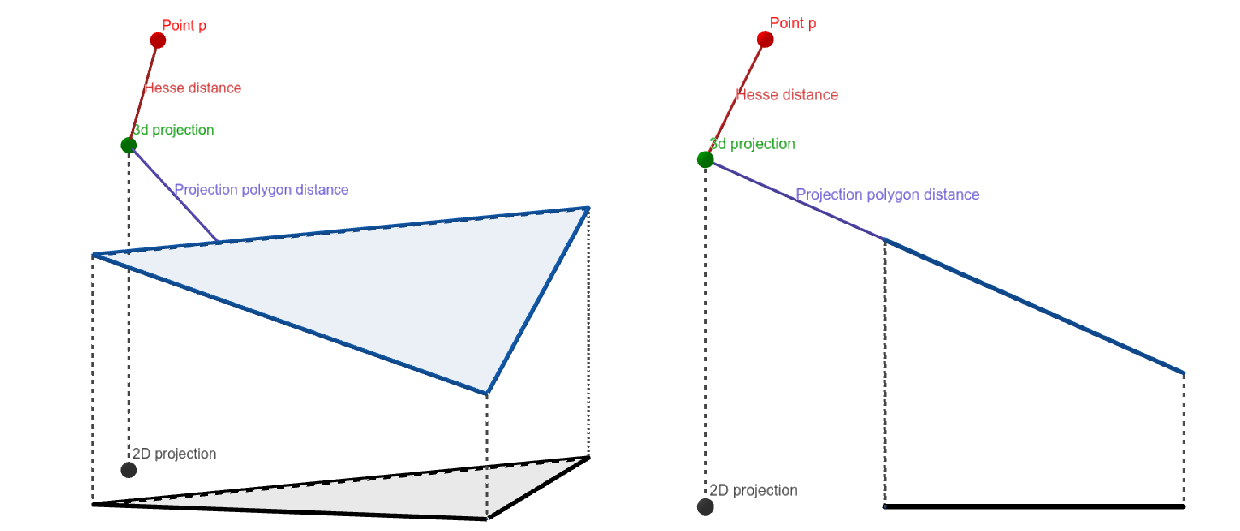
\includegraphics[width=\textwidth]{images/project}
	\caption{\DIFaddFL{Illustration of the Hesse- and polygon projection distance. The point p (red) gets projected onto the infinitely extending global plane. Both the point projection (green) and the global planes convex hull (blue) get projected into 2D space (grey). The Hesse distance, i.e. the shortest distance to the infinitely extending plane (red), is shown as well as the minimum distance from the 2D point projection to the polygon (purple).}}
	\label{fig:proj}
\end{figure*}

\DIFadd{The Hesse-normal form describes the distance from the $i$-th transformed point $T(\vec{p}_i)$ to infinitely extending, $k$-th plane in 3D vector space
}\begin{align}\DIFadd{\label{eq:hesse}
	D_{h}^{i,k} = \vec{n}_{\mathcal{P}_k} \cdot \left[ T(\vec{p}_i) - \vec{a}_{\mathcal{P}_k} \right] ,
}\end{align}
\DIFadd{with normal $\vec{n}_{\mathcal{P}_k}$ and supporting point $\vec{a}_{\mathcal{P}_k}$ of the $k$-th plane.
The distance $D_{h}^{i,k}$ of the $i$-th point to the $k$-th plane reflects the length of the line segment, constructed from the $i$-th point to its projection on the $k$-th plane.
Therefore, by definition the line segment is parallel to the normal vector of the plane.
Thus, the $i$-th points projection $\widetilde{T}(\vec{p}_i)$ onto the $k$-th plane}\DIFaddend , which is \DIFdelbegin \DIFdel{why a simple algorithm is sufficient:
For each plane , consider adding a correspondence for all points closer to the plane than a threshold $\epsilon$.
Depending on the threshold value, some points now have multiple correspondences if their distance to multiple planes is less than $\epsilon$.
We then omit all points with correspondences to multiple planesfrom the optimization to avoid introducing errors due to the plane ambiguity}\DIFdelend \DIFaddbegin \DIFadd{required later, is easily calculated by shifting the point against normal direction:
}\begin{align}\DIFadd{\label{eq:projection}
	\widetilde{T}(\vec{p}_i) = T(\vec{p}_i) - D_{h}^{i,k} \vec{n}_{\mathcal{P}_k}
}\end{align}

\DIFadd{The simplicity of the Hesse distance is at contrast with its inability to take the extent of the plane into account.
Therefore, a second distance model is introduced: the polygon projection distance (PPD).
The convex hull represents the extend of a plane by forming a polygon with the outer most points that are assigned to a given plane. 
It is able to represent the expansion of the plane in all directions, and thus is utilized as a distance model.
To find the PPD, first a corresponding point gets projected onto the infinitely extending plane representation given by the Hesse form, i.e. $\widetilde{T}(\vec{p}_k)$ is found from eq.~}\eqref{eq:projection} \DIFadd{(green point in~\ref{fig:proj}).
Then, the 3D polygon, i.e. the points that make up the convex hull, as well as the corresponding 3D point projection, are projected again into a 2D vector space, using the maximal component of the normal vector of the plane.
E.g. in figure~\ref{fig:proj}, the blue planes normal vector has its mayor component in z-direction (upwards), thus the projection polygon distance is calculated in the xy-plane.
Using the maximum of the absolute magnitude of the normal vector ensures that the most sensible 2D projection is used for every direction.
Sunday et al.~\mbox{%DIFAUXCMD
\cite{pga} }\hspace{0pt}%DIFAUXCMD
presents an optimal algorithm to check whether the point projection lies inside the polygon in 2D. 
If the point is inside the polygon, its PPD is set to zero.
If, however, the point is outside the polygon, the shortest distance to the polygon is calculated by looking at the minimum distance of the $i$-th point to each line segment, making up the convex hull of the $k$-th plane in 3D.
Let the polygon $P_k$ be made up of line segments $s_{m, j}$.
The line segment $s_{m, j}$ consists of the points $p_m$ and $p_j$.
The line segment is parameterized by
}\begin{align}
\DIFadd{\label{eq:line}
	s_{m, j}(t) = p_m + t \cdot \left( p_j - p_m \right) ,  
}\end{align}
\DIFadd{where $t \in \left[ 0, 1 \right]$. 
We set up a distance function, which measures the distance from the query point $p_i$ to an arbitrary point on the line segment.
}\begin{align}
	\DIFadd{\label{eq:dist}
	d_{m, j}(t) = \lVert s_{m, j}(t) - p_i \rVert 
}\end{align} 
\DIFadd{It is now possible to find the shortest distance to the line segment by finding the argument of the function that minimizes this distance.
Therefore, we set
}\begin{align}
	\DIFadd{\pardiff{t} d_{m, j}(t)^2 \overset{!}{=} 0 ,
}\end{align}  
\DIFadd{resulting in 
}\begin{align}
	\DIFadd{t_0 = \frac{\left( p_j - p_m \right) \cdot \left( p_i - p_m \right)}{\left( p_j - p_m \right)^2} .
}\end{align}
\DIFadd{Note the possibility of $t_0 \notin \left[ 0, 1 \right]$. 
In that case, the projection of the point $p_i$ onto the line given by eq.~\ref{eq:line} is not between $p_j$ and $p_m$. 
Instead, its projection onto the line falls outside of the segment.
By constraining $t_0$ we get 
}\begin{align}
\DIFadd{\label{eq:minmax}
	\hat t = \min \left( \max \left( t_0, 0\right) , 1 \right) ,
}\end{align}
\DIFadd{which is the argument that gives the shortest distance to the line segment, when inserted to eq. \ref{eq:dist}.
We find the PPD from the point $p_i$ to the polygon $P_k$ by calculating the minimum shortest distance over all line segments that make up the polygon.  
}

\subsubsection{\DIFadd{Local Planar Clustering}}

\DIFadd{The presented algorithm employs LPC on each individual line scan.
The idea is to find planar features utilizing an optimized approximate k nearest neighbor (AKNN) search for normal calculation as in~\mbox{%DIFAUXCMD
\cite{aknnbbs}}\hspace{0pt}%DIFAUXCMD
.
Thus, normals are calculated for every point in the respective line scan.
Then, the local normal model is combined with a region growing approach.
The region growing is implemented by storing the k-nearest neighbors in a queue, which represents the iteration order of the clustering algorithm.
A region grows if one of these neighbors has a distance shorter then a threshold $d_{growth}$ and additionally has a similar normal.
We define similarity of two normals via the angle between them, which is:
}\begin{align}
\DIFadd{\label{eq:smallestalpha}
	\alpha(\vec{n}_1, \vec{n}_2) = \arccos(\vec{n}_1 \cdot \vec{n}_2) \; .
}\end{align}
\DIFadd{However, the }\textit{\DIFadd{smallest}} \DIFadd{angle between two }\textit{\DIFadd{normal}} \DIFadd{vectors is 
}\begin{align}
\DIFadd{\label{eq:alphahat}
\hat \alpha(\vec{n}_1, \vec{n}_2) = 
\begin{cases}
	2\pi - \alpha(\vec{n}_1, \vec{n}_2) & \text{if  } \alpha(\vec{n}_1, \vec{n}_2) > \frac{3}{2} \pi \\
	\alpha(\vec{n}_1, \vec{n}_2) - \pi & \text{if  } \alpha(\vec{n}_1, \vec{n}_2) > \pi \\
	\pi - \alpha(\vec{n}_1, \vec{n}_2) & \text{if  } \alpha(\vec{n}_1, \vec{n}_2) > \frac{\pi}{2} 
\end{cases}
\; ,
}\end{align}
\DIFadd{because the opposing normals $-\vec{n}_1$ and $-\vec{n}_2$ always have to be considered, since they correspond to the same plane.
We say that two normals are similar if the angle $\hat \alpha$ from eq. \ref{eq:alphahat} is smaller than a threshold $\epsilon_{\alpha}$. 
}

\DIFadd{Planar areas like walls are therefore connected in one large cluster, while non-feature parts, i.e. non-planar or detached parts of the scan will have their own, smaller cluster.
Finally the clusters are filtered in two steps.
First, to combine clusters that are similar, i.e. have a short distance ($d_{growth}$) to each other and similar mean normals (similarity defined as before).
Second, to filter out all clusters that contain non-feature points.
Since all the non-feature points belong to small clusters, the presented algorihtm does this by putting a minimum threshold $N_{c,min}$ on the cluster size.
Figure \ref{fig:clustering} shows this concept on the real world dataset described later in section \ref{sec:experimentalSetup}.
}

\begin{figure*}
	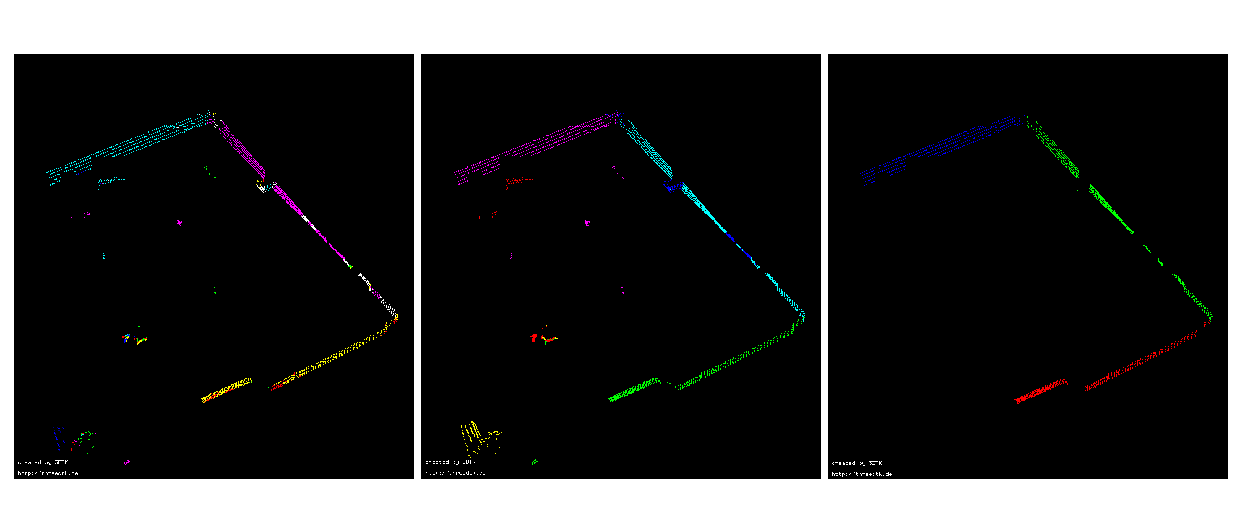
\includegraphics[width=\linewidth]{images/clustering}
	\caption{\DIFaddFL{(Left) Point normals using the AKNN method with $K = 20$. (Middle) Result of the region growing, before applying the second filter. (Right) Resulting clusters after applying the second filter, using $N_{c,min} = 300$. }}
	\label{fig:clustering}
\end{figure*}

\DIFadd{Point-to-Plane correspondences are now established.
The distance models (Hesse and PPD) are utilized to check whether a cluster overlaps with any of the global planes, i.e. any point in the cluster has a Hesse distance smaller than some threshold $\epsilon_H$ and a PPD smaller than some additional threshold $\epsilon_P$, to the global plane.
We observe the noise level around the expected planes by the naked eye. 
Then we set the thresholds accordingly. 
For each overlap, we find the smallest angle between the corresponding cluster normal and the global plane normal, according to eq. \ref{eq:alphahat}.
Finally, a correspondence is established between all points in the cluster and the global plane, if the minimum angle between their normals is smaller than $\epsilon_\alpha$}\DIFaddend . 

\subsection{Optimization}

Assuming we \DIFdelbegin \DIFdel{know now }\DIFdelend \DIFaddbegin \DIFadd{now know }\DIFaddend the Hesse-normal form of all planes and all assigned points to these planes, we register the points to have a minimal distance to their respective planes.
The transformation \DIFdelbegin \DIFdel{$T(\vec{p}_k)$ }\DIFdelend \DIFaddbegin \DIFadd{$T(\vec{p}_i)$ }\DIFaddend of each point \DIFdelbegin \DIFdel{$\vec{p}_k$ }\DIFdelend \DIFaddbegin \DIFadd{$\vec{p}_i$ }\DIFaddend with respect to a 6 DoF motion is described in homogeneous coordinates using the roll-pitch-yaw ($\varphi-\vartheta-\psi$) Tait-Brian angles as in~\cite{diebel2006representing}. Transforming the result back from homogeneous coordinates and using \DIFdelbegin \DIFdel{$C_k$ and $S_k$ }\DIFdelend \DIFaddbegin \DIFadd{$C_a$ and $S_a$ }\DIFaddend to denote the cosine and sine of the angle in the subscript\DIFdelbegin \DIFdel{yields:
}\DIFdelend \DIFaddbegin \DIFadd{, and $t_a$ denoting the translation along the axis in the subscript yields:
}\DIFaddend \begin{align}
	T(\vec{p}\DIFdelbegin \DIFdel{_k}\DIFdelend \DIFaddbegin \DIFadd{_i}\DIFaddend )  =
    \DIFdelbegin %DIFDELCMD < \resizebox{0.35\textwidth}{!}{$\begin{bmatrix}
%DIFDELCMD <         x C_\vartheta C_\psi - yC_\varphi S_\psi + z S_\vartheta + t_x\\
%DIFDELCMD <         x (C_\varphi S_\psi + C_\psi S_\varphi S_\vartheta) + y(C_\varphi C_\psi - S_\varphi S_\vartheta S_\psi) - z C_\vartheta S_\varphi + t_y\\
%DIFDELCMD <         x(S_\varphi S_\psi - C_\varphi C_\psi S_\vartheta) + y(C_\psi S_\varphi + C_\varphi S_\vartheta S_\psi) + z C_\varphi C_\vartheta + t_z
%DIFDELCMD <     \end{bmatrix}$}
%DIFDELCMD < %%%
\DIFdelend \DIFaddbegin \resizebox{0.35\textwidth}{!}{%
\mbox{%DIFAUXCMD
$\begin{bmatrix}
        x_i C_\vartheta C_\psi - y_iC_\vartheta S_\psi + z_i S_\vartheta + t_x\\
        x_i (C_\varphi S_\psi + C_\psi S_\varphi S_\vartheta) + y_i(C_\varphi C_\psi - S_\varphi S_\vartheta S_\psi) - z_i C_\vartheta S_\varphi + t_y\\
        x_i(S_\varphi S_\psi - C_\varphi C_\psi S_\vartheta) + y_i(C_\psi S_\varphi + C_\varphi S_\vartheta S_\psi) + z_i C_\varphi C_\vartheta + t_z
    \end{bmatrix}$
}%DIFAUXCMD
}
\DIFaddend \end{align}
From this we define the function \DIFdelbegin \DIFdel{$D(\varphi,\vartheta,\psi,t_x,t_y,t_z, \vec{p}_k)$ }\DIFdelend \DIFaddbegin \DIFadd{$D(\varphi,\vartheta,\psi,t_x,t_y,t_z, \vec{p}_{i})$ }\DIFaddend that computes the distance of a point \DIFdelbegin \DIFdel{$\vec{p}_k$ }\DIFdelend \DIFaddbegin \DIFadd{$\vec{p}_{i}$ }\DIFaddend to its corresponding plane \DIFdelbegin \DIFdel{$\mathcal{P}_i$}\DIFdelend \DIFaddbegin \DIFadd{$\mathcal{P}_k$}\DIFaddend .
Omitting the arguments of the function for simplicity:
\begin{align}
\DIFdelbegin %DIFDELCMD < \begin{aligned}
%DIFDELCMD <     D &= T(\vec{p}_k) \cdot \vec{n}_{\mathcal{P}_i} \\
%DIFDELCMD <       &= n_{\mathcal{P}_i}^x (x C_\vartheta C_\psi - yC_\varphi S_\psi + z S_\vartheta + t_x)\\
%DIFDELCMD <        &+ n_{\mathcal{P}_i}^y(x (C_\varphi S_\psi + C_\psi S_\varphi S_\vartheta)\\
%DIFDELCMD <        &\qquad+ y(C_\varphi C_\psi - S_\varphi S_\vartheta S_\psi) - z C_\vartheta S_\varphi + t_y)\\
%DIFDELCMD <        &+ n_{\mathcal{P}_i}^z (x(S_\varphi S_\psi - C_\varphi C_\psi S_\vartheta)\\
%DIFDELCMD <        &\qquad+ y(C_\psi S_\varphi + C_\varphi S_\vartheta S_\psi) + z C_\varphi C_\vartheta + t_z)\\
%DIFDELCMD <        &- \rho_{\mathcal{P}_i}
%DIFDELCMD < \end{aligned}%%%
\DIFdelend \DIFaddbegin \begin{aligned}
    D &= T(\vec{p}_i) \cdot \vec{n}_{\mathcal{P}_k} \\
      &= n_{\mathcal{P}_k}^x (x_i C_\vartheta C_\psi - y_iC_\vartheta S_\psi + z_i S_\vartheta + t_x)\\
       &+ n_{\mathcal{P}_k}^y(x_i (C_\varphi S_\psi + C_\psi S_\varphi S_\vartheta)\\
       &\qquad+ y_i(C_\varphi C_\psi - S_\varphi S_\vartheta S_\psi) - z_i C_\vartheta S_\varphi + t_y)\\
       &+ n_{\mathcal{P}_k}^z (x_i(S_\varphi S_\psi - C_\varphi C_\psi S_\vartheta)\\
       &\qquad+ y_i(C_\psi S_\varphi + C_\varphi S_\vartheta S_\psi) + z_i C_\varphi C_\vartheta + t_z)\\
       &- \rho_{\mathcal{P}_k}
\end{aligned}\DIFaddend 
\end{align}

This distance function is what we want to minimize for all points and their respective planes.
Hence the error function $E$ is chosen as \DIFdelbegin \DIFdel{follows:
}\DIFdelend \DIFaddbegin \DIFadd{the square of the L2-norm of the distance:
}\DIFaddend \begin{align}
	E = \sum\DIFdelbegin \DIFdel{_{\forall \mathcal{P}_i}}\DIFdelend \DIFaddbegin \DIFadd{_{\forall \mathcal{P}_k}}\DIFaddend \sum\DIFdelbegin \DIFdel{_{\vec{p}_k \in \mathcal{P}_i} }%DIFDELCMD < \norm[2]{D(\varphi,\vartheta,\psi,t_x,t_y,t_z, \vec{p}_k)}%%%
\DIFdelend \DIFaddbegin \DIFadd{_{\vec{p}_i \in \mathcal{P}_k} }\norm[2]{D(\varphi,\vartheta,\psi,t_x,t_y,t_z, \vec{p}_i)}\DIFaddend ^2
\end{align}
Its gradient follows then immediately:
\begin{align}
	&\nabla E =  \sum\DIFdelbegin \DIFdel{_{\forall \mathcal{P}_i}}\DIFdelend \DIFaddbegin \DIFadd{_{\forall \mathcal{P}_k}}\DIFaddend \sum\DIFdelbegin \DIFdel{_{\vec{p}_k \in \mathcal{P}_i} }\DIFdelend \DIFaddbegin \DIFadd{_{\vec{p}_i \in \mathcal{P}_k} }\DIFaddend \resizebox{0.28\textwidth}{!}{$\begin{bmatrix}\pardiff{\varphi} E&\pardiff{\vartheta} E&\pardiff{\psi} E&\pardiff{t_x} E&\pardiff{t_y} E&\pardiff{t_z} E\end{bmatrix}^T$}\\
    &\Rightarrow\nabla E = \DIFdelbegin %DIFDELCMD < \resizebox{0.35\textwidth}{!}{$\sum_{\forall \mathcal{P}_i} \sum_{\vec{p}_k \in \mathcal{P}_i}2D(\vec{\Pi}, \vec{p}_k)\begin{bmatrix}\nabla E_\varphi &\nabla E_\vartheta & \nabla E_\psi & n_{\mathcal{P}_i}^x&n_{\mathcal{P}_i}^y&n_{\mathcal{P}_i}^z\end{bmatrix}^T$}
%DIFDELCMD < %%%
\DIFdelend \DIFaddbegin \resizebox{0.35\textwidth}{!}{%
\mbox{%DIFAUXCMD
$\sum_{\forall \mathcal{P}_k} \sum_{\vec{p}_i\in \mathcal{P}_k}2D(\vec{\Pi}, \vec{p}_i)\begin{bmatrix}\nabla E_\varphi &\nabla E_\vartheta & \nabla E_\psi & n_{\mathcal{P}_k}^x&n_{\mathcal{P}_k}^y&n_{\mathcal{P}_k}^z\end{bmatrix}^T$
}%DIFAUXCMD
}
\DIFaddend \end{align}
Where
\begin{align}
&\DIFdelbegin %DIFDELCMD < \begin{alignedat}{3}
%DIFDELCMD <         %%%
\DIFdel{\nabla E_\varphi = }%DIFDELCMD < & %%%
\DIFdel{n_{\mathcal{P}_i}^x}%DIFDELCMD < &&%%%
\DIFdel{y S_\varphi S_\psi }%DIFDELCMD < \\
%DIFDELCMD <         &%%%
\DIFdel{+ n_{\mathcal{P}_i}^y}%DIFDELCMD < &&%%%
\DIFdel{(x}%DIFDELCMD < [%%%
\DIFdel{-S_\varphi S_\psi+C_\varphi C_\psi S_\vartheta}%DIFDELCMD < ] \\&&&%%%
\DIFdel{+y}%DIFDELCMD < [%%%
\DIFdel{-S_\varphi C_\psi -C_\varphi S_\vartheta S\psi}%DIFDELCMD < ] \\&&&%%%
\DIFdel{- z C_\varphi C_\vartheta)}%DIFDELCMD < \\
%DIFDELCMD <         &%%%
\DIFdel{+ n_{\mathcal{P}_i}^z}%DIFDELCMD < &&%%%
\DIFdel{(x}%DIFDELCMD < [%%%
\DIFdel{C_\varphi S_\psi+C_\varphi C_\psi S_\vartheta}%DIFDELCMD < ] \\&&&%%%
\DIFdel{+y}%DIFDELCMD < [%%%
\DIFdel{C_\varphi C_\psi -S_\varphi S_\vartheta S\psi}%DIFDELCMD < ] \\&&&%%%
\DIFdel{- z S_\varphi C_\vartheta)
    }%DIFDELCMD < \end{alignedat} \\
%DIFDELCMD <     &\begin{alignedat}{3}
%DIFDELCMD <         %%%
\DIFdel{\nabla E_\vartheta = }%DIFDELCMD < & %%%
\DIFdel{n_{\mathcal{P}_i}^x(-xS_\vartheta C_\psi + zC_\vartheta) }%DIFDELCMD < \\
%DIFDELCMD <         &%%%
\DIFdel{+ n_{\mathcal{P}_i}^y(xC_\psi S_\varphi C_\vartheta - yS_\varphi C_\vartheta S_\psi + z S_\vartheta S_\varphi)  }%DIFDELCMD < \\
%DIFDELCMD <         &%%%
\DIFdel{+ n_{\mathcal{P}_i}^z(-xC_\varphi C_\psi C_\vartheta + yC_\varphi C_\vartheta S_\psi - z C_\varphi S_\vartheta)
    }%DIFDELCMD < \end{alignedat}\\
%DIFDELCMD <     &\begin{alignedat}{3}
%DIFDELCMD <        %%%
\DIFdel{\nabla E_\psi =}%DIFDELCMD < & %%%
\DIFdel{n_{\mathcal{P}_i}^x}%DIFDELCMD < &&\left(%%%
\DIFdel{-xC_\vartheta S_\psi - yC_\varphi C_\psi}%DIFDELCMD < \right) \\
%DIFDELCMD <        &%%%
\DIFdel{+ n_{\mathcal{P}_i}^y}%DIFDELCMD < &&%%%
\DIFdel{(x}%DIFDELCMD < [%%%
\DIFdel{C_\varphi C_\psi - S_\varphi S_\vartheta S_\psi}%DIFDELCMD < ] \\
%DIFDELCMD <        &&&%%%
\DIFdel{+ y}%DIFDELCMD < [%%%
\DIFdel{-C_\varphi S_\psi - S_\varphi S_\theta C_\psi}%DIFDELCMD < ]%%%
\DIFdel{) }%DIFDELCMD < \\
%DIFDELCMD <        &%%%
\DIFdel{+ n_{\mathcal{P}_i}^z}%DIFDELCMD < &&%%%
\DIFdel{(x}%DIFDELCMD < [%%%
\DIFdel{S_\varphi C_\psi + C_\varphi S_\psi S_\theta}%DIFDELCMD < ] \\
%DIFDELCMD <        &&&%%%
\DIFdel{+ y}%DIFDELCMD < [%%%
\DIFdel{-S_\psi S_ \varphi + C_\varphi S_\vartheta C_\psi}%DIFDELCMD < ]%%%
\DIFdel{) 
    }%DIFDELCMD < \end{alignedat}
%DIFDELCMD < %%%
\DIFdelend \DIFaddbegin \begin{aligned}
\nabla E_\varphi = &n_{\mathcal{P}_k}^y(x_i[-S_\varphi S_\psi+C_\varphi C_\psi S_\vartheta]\\
			       & +y_i[-S_\varphi C_\psi -C_\varphi S_\vartheta S\psi] - z_i C_\varphi C_\vartheta)\\
                   &+ n_{\mathcal{P}_k}^z(x_i[C_\varphi S_\psi+C_\varphi C_\psi S_\vartheta] \\
                   &+y_i[C_\varphi C_\psi -S_\varphi S_\vartheta S\psi] - z_i S_\varphi C_\vartheta)
\end{aligned} \DIFadd{\;\; ,
}\DIFaddend \end{align}
\DIFaddbegin \begin{align}
&\DIFadd{\begin{aligned}
\nabla E_\vartheta = & n_{\mathcal{P}_k}^x(-x_iS_\vartheta C_\psi + y_i S_\vartheta S_\psi + z_iC_\vartheta) \\
        &+ n_{\mathcal{P}_k}^y(x_iC_\psi S_\varphi C_\vartheta - y_iS_\varphi C_\vartheta S_\psi + z_i S_\vartheta S_\varphi)  \\
        &+ n_{\mathcal{P}_i}^z(-x_iC_\varphi C_\psi C_\vartheta + y_iC_\varphi C_\vartheta S_\psi - z_i C_\varphi)
\end{aligned}\;\; ,}\\
&\DIFadd{\begin{aligned}
	\nabla E_\psi = &n_{\mathcal{P}_k}^x\left(-x_iC_\vartheta S_\psi - y_iC_\vartheta C_\psi\right) \\
       &+ n_{\mathcal{P}_k}^y(x_i[C_\varphi C_\psi - S_\varphi S_\vartheta S_\psi]\\
       &\quad+ y_i[-C_\varphi S_\psi - S_\varphi S_\theta C_\psi]) \\
       &+ n_{\mathcal{P}_k}^z(x_i[S_\varphi C_\psi + C_\varphi S_\psi S_\theta] \\
       &\quad+ y_i[-S_\psi S_ \varphi + C_\varphi S_\vartheta C_\psi]) 
\end{aligned}
}\end{align}
\DIFaddend and $\vec{\Pi}=\begin{bmatrix}\varphi & \vartheta & \psi & t_x & t_y & t_z\end{bmatrix}^T$.

As the gradient is well-defined we minimize the error function with any gradient based method. 
The commonly used, well-known stochastic gradient descent (SDG) algorithm computes 
\begin{align}
    \vec{\Pi}_{k+1} = \vec{\Pi}_{k} - \alpha \nabla E
\end{align}
\DIFaddbegin \DIFadd{where $\alpha$ is the learning rate.
}\DIFaddend To accelerate convergence and to improve the found solution further modifications are made.

Since we have vastly different effects on the error function by each dimension, the first consideration for improving the SDG is the following:
Typically, changes in orientation, i.e., the first three elements of the gradient vector $\pardiff{\varphi}E$, $\pardiff{\vartheta}E$, and $\pardiff{\psi}E$, have much more impact on the error function than a change in position.
This is intuitively explained since translating the scan makes the error grow linearly for all points.
However, when rotating the scan, points with a larger distance to the robot are moved drastically, leading to a higher sensibility on the error function.
For this reason, the $\alpha$ applied on orientation has to be much smaller than the $\alpha$ applied on the position.
It becomes obvious that $\alpha$ needs to be extended into vector form, $\boldsymbol\alpha$, therefore weighting each dimension differently.

Another consideration to speed up SDG is to adaptively recalculate $\boldsymbol\alpha$ for each iteration. 
We employ and modify ADADELTA as a technique to do so, which is described in detail in~\cite{zeiler2012adadelta}.
The main idea is the following:
It extends the SDG algorithm by two terms.
First, an exponentially decaying average of past gradients \DIFaddbegin \DIFadd{$\vec{G}_k$}\DIFaddend , which is recursively defined as
\begin{align}
    \vec{G}_{k+1} = \DIFdelbegin \DIFdel{\rho }\DIFdelend \DIFaddbegin \DIFadd{\zeta }\DIFaddend \vec{G}_{k} + (1 - \DIFdelbegin \DIFdel{\rho}\DIFdelend \DIFaddbegin \DIFadd{\zeta}\DIFaddend ) {\nabla E}^2
\end{align}
and second, an exponentially decaying average of past changes \DIFaddbegin \DIFadd{$\vec{X}_k$}\DIFaddend , which is defined as
\begin{align}
    \vec{X}_{k+1} = \DIFdelbegin \DIFdel{\rho }\DIFdelend \DIFaddbegin \DIFadd{\zeta }\DIFaddend \vec{X}_{k} + (1 - \DIFdelbegin \DIFdel{\rho}\DIFdelend \DIFaddbegin \DIFadd{\zeta}\DIFaddend ) {\boldsymbol\alpha \nabla E}^2
\end{align}
where \DIFdelbegin \DIFdel{$\rho \leq 1$ }\DIFdelend \DIFaddbegin \DIFadd{$\zeta \leq 1$ }\DIFaddend is a decay constant, typically close to $1$.
The root mean squared (RMS) of these quantities are
\begin{align}
    RMS[\vec{G}]_{k} = \DIFdelbegin \DIFdel{\sqrt{\vec{G}_{k} + \epsilon}
}\DIFdelend \DIFaddbegin \DIFadd{\sqrt{\vec{G}_{k} + \epsilon_{num}}
}\DIFaddend \end{align}
and 
\begin{align}
    RMS[\vec{X}]_{k} = \DIFdelbegin \DIFdel{\sqrt{\vec{X}_{k} + \epsilon}
}\DIFdelend \DIFaddbegin \DIFadd{\sqrt{\vec{X}_{k} + \epsilon_{num}}
}\DIFaddend \end{align}
where \DIFdelbegin \DIFdel{$\epsilon > 0$ }\DIFdelend \DIFaddbegin \DIFadd{$\epsilon_{num} > 0$ }\DIFaddend is a very small constant, typically close to $0$ \DIFaddbegin \DIFadd{(Note: this is a different threshold as the one used in section~\ref{sec:point-to-plane-correspondences})}\DIFaddend .
It will prevent dividing by zero in the recalculation of $\boldsymbol\alpha$, which is as follows:
\begin{align}
    \boldsymbol\alpha_{k} = \frac{RMS[X]_{k-1}}{RMS[G]_{k}}
    \label{eq:adadeltaalphaupdate}
\end{align} 
For our particular application, ADADELTA behaves a little too aggressively.
Despite giving a good measure on how to adapt $\boldsymbol\alpha$, the algorithm sometimes overshoots, and does not converge.
Therefore, we employ another scaling factor, typically not found in ADADELTA, extending eq.~\eqref{eq:adadeltaalphaupdate} to:
\begin{align}
    \boldsymbol\alpha_{k} = \boldsymbol\alpha_0 \cdot \frac{RMS[X]_{k-1}}{RMS[G]_{k}}
    \label{eq:adafinalized}
\end{align} 
where $\boldsymbol\alpha_0 $ holds the scaling factors for each dimension.

Finally, the SDG model is improved using eq.~\eqref{eq:adafinalized} and extends to 
\begin{align}
    \vec{\Pi}_{k+1} = \vec{\Pi}_{k} - \boldsymbol\alpha_0  \frac{RMS[X]_{k-1}}{RMS[G]_{k}} \cdot \nabla E
\end{align}
Using this algorithm once after finding correspondences from points to planes leads to convergence to a local minimum, which is often not an optimal solution.
Even if we increase the number of iterations dramatically, no better solution than the local minimum is found.
That is unless you consider updating the correspondence model after $i$ iterations of gradient descent.
Re-assigning point-to-plane correspondences this way $k$ times, with a large enough $k$, leads to an optimal solution after maximum $n = k\cdot i$ iterations of gradient descent.

\subsection{Further Optimizations of the Algorithm}
\DIFaddbegin \label{ssec:furtheropts}
\DIFaddend 

The algorithm was extended by two further optimizations, which are helpful in different scenarios.

Firstly, we introduce \DIFaddbegin \DIFadd{the possibility to choose }\DIFaddend a lock on some dimensions from being optimized by setting the corresponding $\alpha_i$ to zero.
Although 6D optimization generally works, reducing the optimization space is particularly useful if the source of error in the system is known and a model exists.
That way, e.g., \DIFdelbegin \DIFdel{a point cloud from a terrestrial laserscanner that experiences irregularities in its spinning mirror is registered by optimizing only over the axis of rotation as no other movement is to be expected}\DIFdelend \DIFaddbegin \DIFadd{as we expect a spherical robot to move on a plane the position along the axis perpendicular to the plane is constant and should not be used for optimization}\DIFaddend .

Secondly, we employ a \DIFdelbegin \DIFdel{continuous }\DIFdelend \DIFaddbegin \DIFadd{sequential }\DIFaddend iteration, where the scans are processed \DIFdelbegin \DIFdel{sequentially}\DIFdelend \DIFaddbegin \DIFadd{one after another}\DIFaddend . 
This is especially useful for mobile systems, where pose errors accumulate due to increasing tracking uncertainties.
The assumption is that the error in one scan is also present in the following scan, plus some unknown new error.
We eliminate the error from scan $m$ which is also present in scan $m+1$ by applying the pose change from scan $m$, $\vec{\Pi}_{n,m} - \vec{\Pi}_{0,m}$ after $n$ gradient descent iterations, to scan $m+1$, before restarting gradient descent.

To quantify the quality of the proposed registration method, it is tested on simulated and real-world data. 

%!TEX root = ../main.tex
\section{Simulation}

For the simulated data, we implemented a noisy world-robot-sensor model.  
The simulated sensor is modeled after a Livox-Mid100~\cite{LivoxMid40-100} laser scanner with customizable noise level on the range measurements inside a robot with different motion capabilities, subject to noise in its pose estimation. 
This yields scan results similar to the ones obtained in the real world.

\subsection{Simulated Sensor}

The Livox-Mid100 laser scanner consists of three Mid40 scanners arranged to provide an overall field-of-view of \SI{98.4}{\degree} (horizontal) by \SI{38.4}{\degree} (vertical).
\DIFdelbegin \DIFdel{With a range precision of \mbox{%DIFAUXCMD
\SI{2}{\centi\meter} }\hspace{0pt}%DIFAUXCMD
up to \mbox{%DIFAUXCMD
\SI{20}{\meter} }\hspace{0pt}%DIFAUXCMD
range it provides }\DIFdelend \DIFaddbegin \DIFadd{It provides a rate of }\DIFaddend \SI[per-mode=symbol]{300,000}{\pts\per\second} with a range precision of \SI{2}{\centi\meter} up to \SI{20}{\meter} range\DIFaddbegin \DIFadd{~\mbox{%DIFAUXCMD
\cite{LivoxMid40-100}}\hspace{0pt}%DIFAUXCMD
}\DIFaddend .
A particular advantage of the Livox laser scanners is their unique scanning pattern.
The scanners use two motorized, so-called Risley prisms to steer the beam deflectance.
For the specific ratio of rotation speeds used in the Livox scanners, the beam traces out a non-repetitive, flower-shaped scanning pattern~\cite{thorlabs}.
Since the pattern is non-repetitive, the point density increases with integration time, enabling denser measurements.

\subsection{Range Noise Model}

Most real laser scanners are subjected to range measurement noise that is proportional to the measured range. 
Therefore the simulated sensors are as well. 
To achieve this, we sample a noise percentage $n_P$ from some normal distribution $\mathcal{N}(\mu,\sigma^2)$. 
The resulting range $r$ given the true range $r_t$ is then
\begin{align}
	r = r_t(1+n_P)
\end{align}
For each measurement ray the noise percentage is sampled independently. 

\subsection{Pose Estimation Noise Model} 

Regarding the pose measurement, one cannot simply add white noise to the current pose estimate as this does not capture the integration error, which is common among inertial measurement units (IMU). 
Therefore we assume a disturbance torque about the two axes that lie in the ground plane. 
This is equivalent to a case where a slightly shifted ground plane or an unbalanced locomotion system of the robot is present.  

Accordingly, a spherical robot that is assumed to be translating exactly along one axis by rotating about one other axis at an angular velocity $\omega$  experiences random disturbance torques at each time instant that accelerate the rotation of the sphere about the respective axes. 
This additional motion is determined by integrating the disturbance torques, which are sampled from some normal distribution $n_\phi, n_\psi \in \mathcal{N}(\mu,\sigma^2)$ each.  
The pose update \DIFdelbegin \DIFdel{in the discrete }\DIFdelend \DIFaddbegin \DIFadd{after a discrete time step $\Delta t$ in the }\DIFaddend simulation is therefore given by: 
\begin{align}
	\begin{bmatrix}\varphi\\\vartheta\\\psi\\x\\y\\z\end{bmatrix}_{k+1} = 
	\begin{bmatrix}\varphi\\\vartheta\\\psi\\x\\y\\z\end{bmatrix}_{k} 
	+ \DIFdelbegin %DIFDELCMD < \begin{bmatrix}1\\0\\0\\R\\0\\0\end{bmatrix}%%%
\DIFdelend \DIFaddbegin \begin{bmatrix}1\\0\\0\\0\\0\\R\end{bmatrix}\DIFaddend \omega \Delta t  + \Delta t \DIFdelbegin %DIFDELCMD < \underbrace{\sum_{i = 0}^k \begin{bmatrix}n_\varphi[i] \Delta t\\0\\n_\psi[i]\Delta t\\0\\0\\0\end{bmatrix}}%%%
\DIFdelend \DIFaddbegin \underbrace{\sum_{i = 0}^k \begin{bmatrix}n_\varphi[i] \Delta t\\0\\n_\psi[i]\Delta t\\n_\varphi[i] \Delta t R\\0\\n_\psi[i]\Delta tR\end{bmatrix}}\DIFaddend _{\substack{\text{Difference in}\\\text{angular velocity}}}
\end{align}
\DIFaddbegin \DIFadd{where $\Delta t$ is generally chosen as some small value (e.g. \mbox{%DIFAUXCMD
\SI{1}{\milli\second}}\hspace{0pt}%DIFAUXCMD
)
}\DIFaddend 

Assuming intended locomotion along the $z$-axis and unintended locomotion along the $x$-axis where $R$ is the sphere radius.
No upwards movement is possible since the robot moves on a flat ground, hence the entry is zero.

\subsection{Simulated Datasets}

Figure~\ref{fig:simulatedDatasets} shows a noise-free trajectory through a simulated environment and a trajectory with noisy sensors while figure~\ref{fig:robotRender} shows a rendering of the \DIFdelbegin \DIFdel{simulated robot as well as the }\DIFdelend simulation sequence.
In the noise-free case, the trajectory slightly bends in the direction of disturbance torque sideways while also varying in velocity in the intended direction of travel.
In the noisy case, the ideal straight trajectory is assumed.
Hence the planes enclosing the room are sensed multiple times. 
In particular, we see that the trajectory of the robot leads through one of the sensed planes. 
Also, the further the sensed points are, the noisier they appear, which is consistent with the larger influence of the pose error at higher distances.  

\begin{figure*}
	\centering
	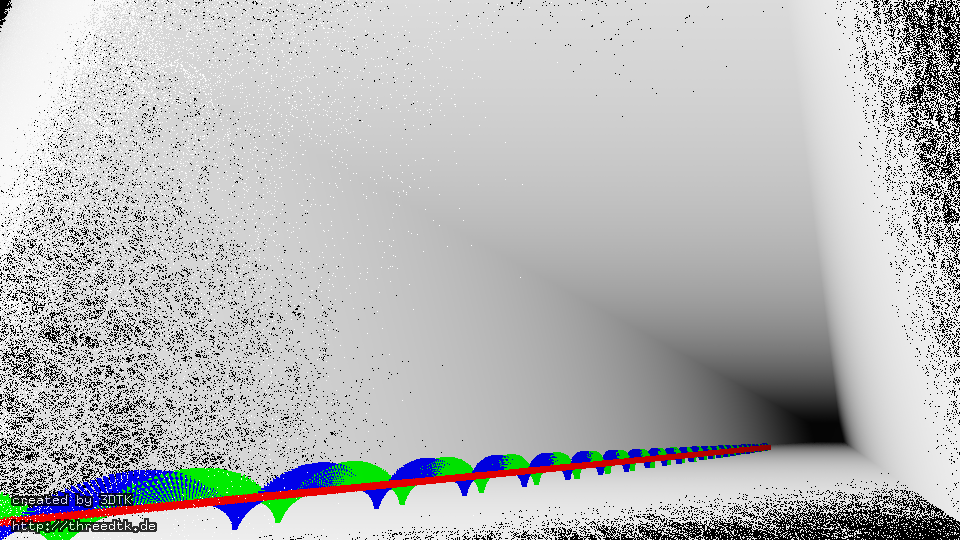
\includegraphics[width=0.495\textwidth]{images/perfect_bottom}\hfill
	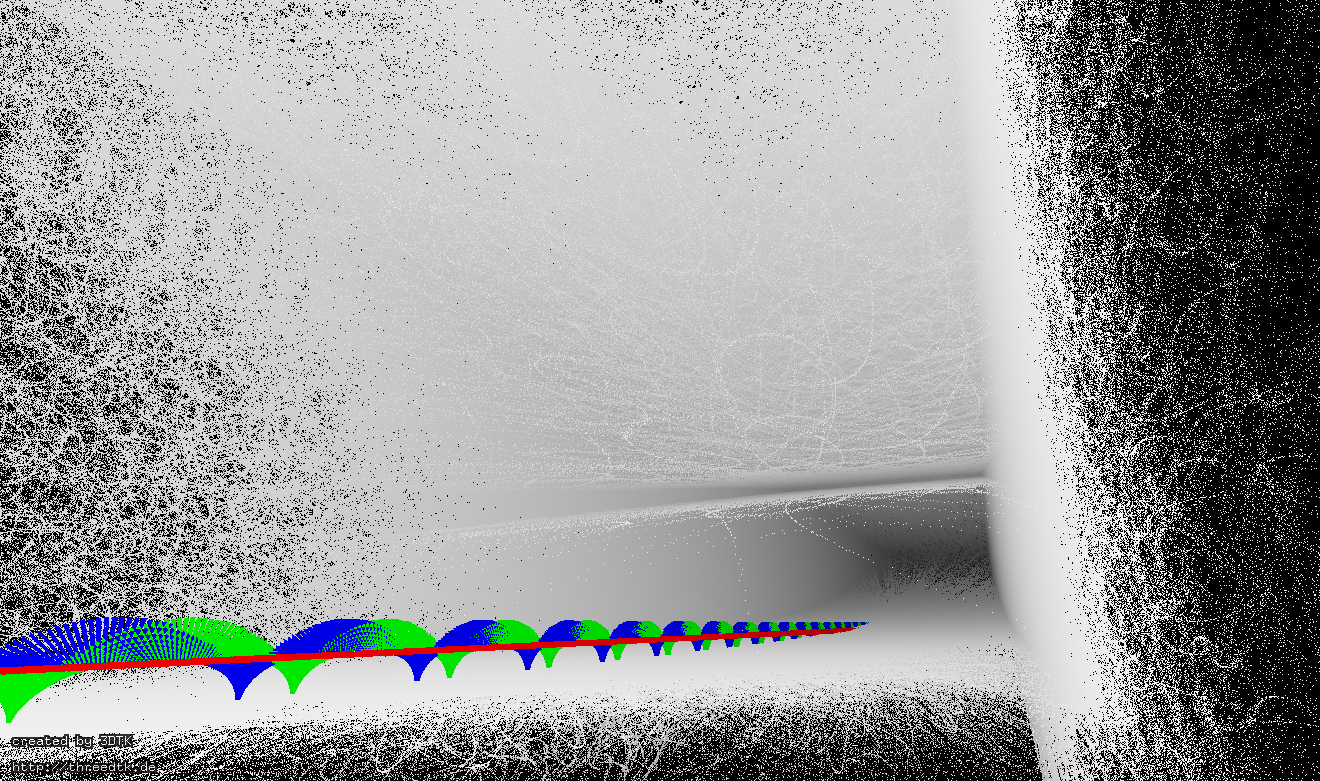
\includegraphics[width=0.495\textwidth]{images/noisy_pose_and_range_bottom}\\
	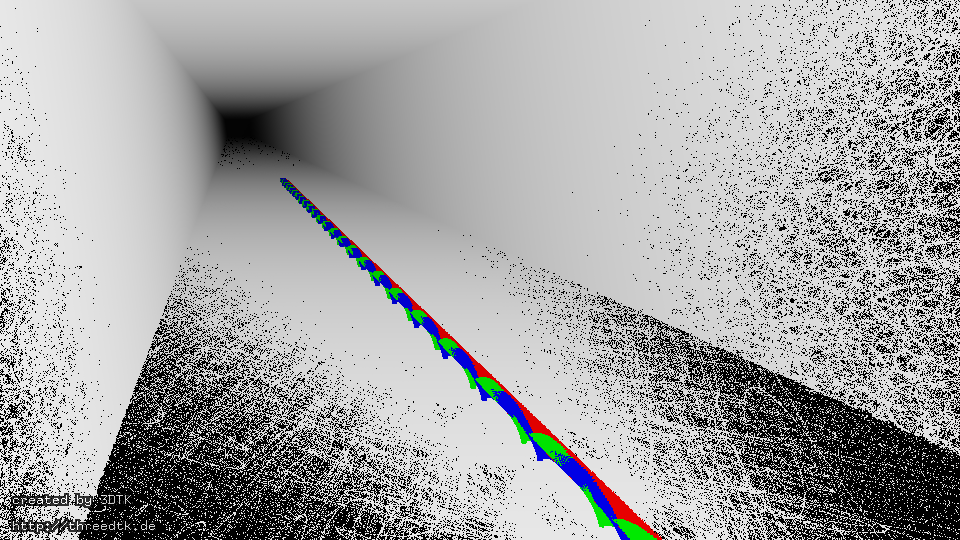
\includegraphics[width=0.495\textwidth]{images/perfect_top}\hfill
	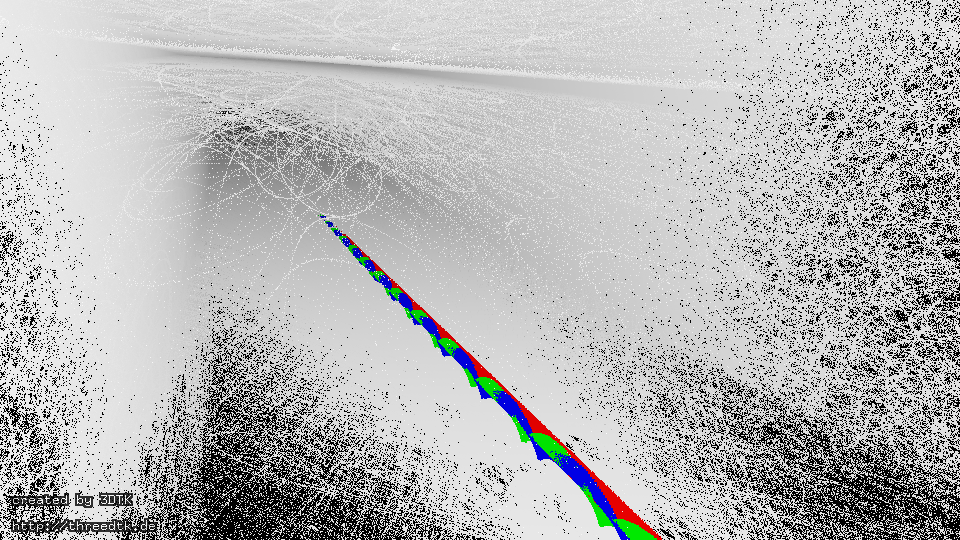
\includegraphics[width=0.495\textwidth]{images/noisy_pose_and_range_top}\\
	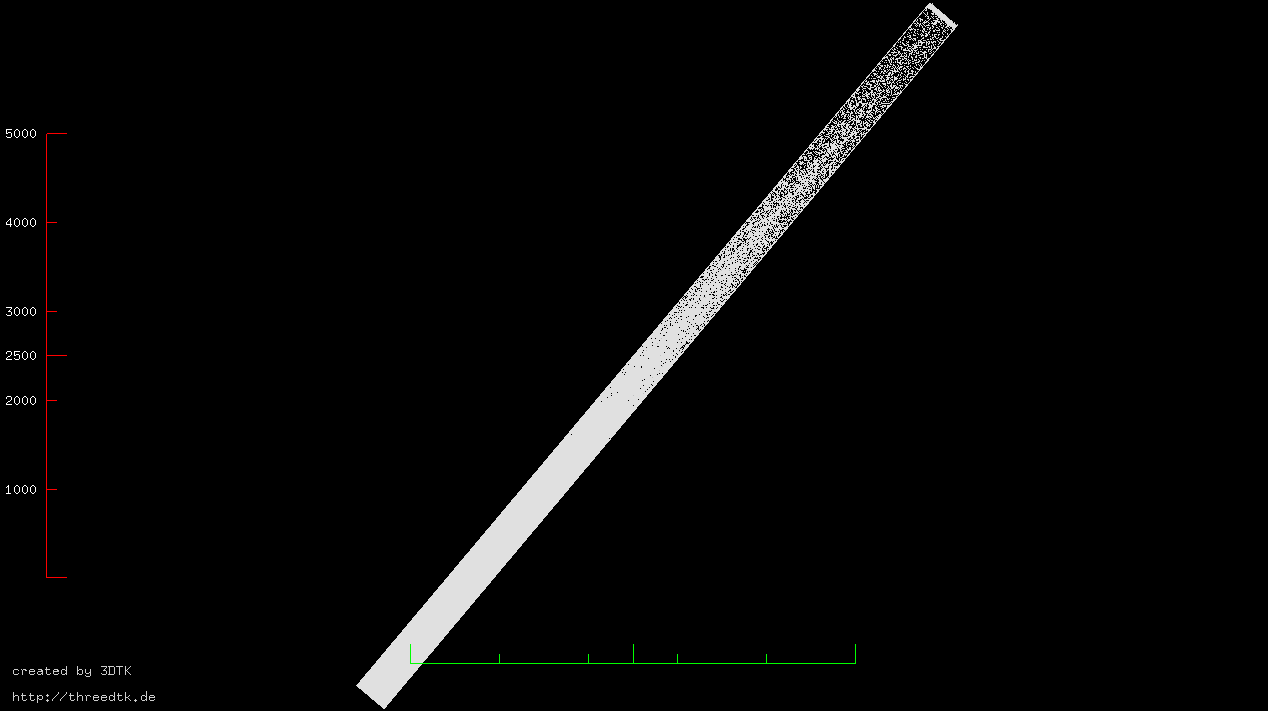
\includegraphics[width=0.495\textwidth]{images/perfect_top_view}\hfill
	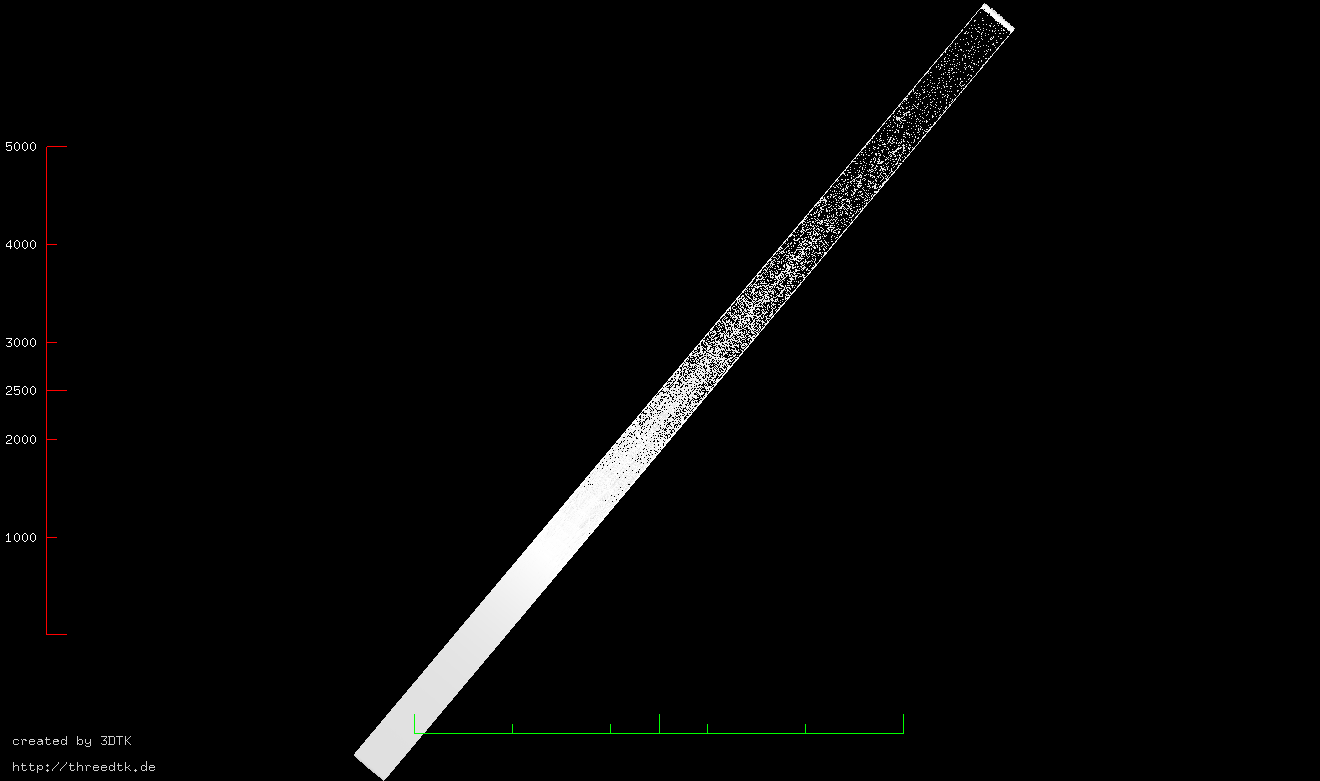
\includegraphics[width=0.495\textwidth, height=0.1825\textwidth]{images/noisy_pose_and_range_top_view}
	\caption{Two simulated datasets of a long hallway of size $\SI{4}{\meter}\times\SI{3}{\meter}\times\SI{100}{\meter}$. Ideal noise free (left), noisy pose ($\mathcal{N}_\varphi = \mathcal{N}_\psi(\mu = 0.0001, \sigma= 0.00001)$) and noisy range measurements ($\mathcal{N}_r(\mu = 0, \sigma = 0.001)$) (right). 
	\DIFaddbeginFL \DIFaddFL{The normal distributions are define in such a way, that in the resulting dataset plane detection is still possible.}\DIFaddendFL }
	\label{fig:simulatedDatasets}
\end{figure*}

\begin{figure*}
	\centering
	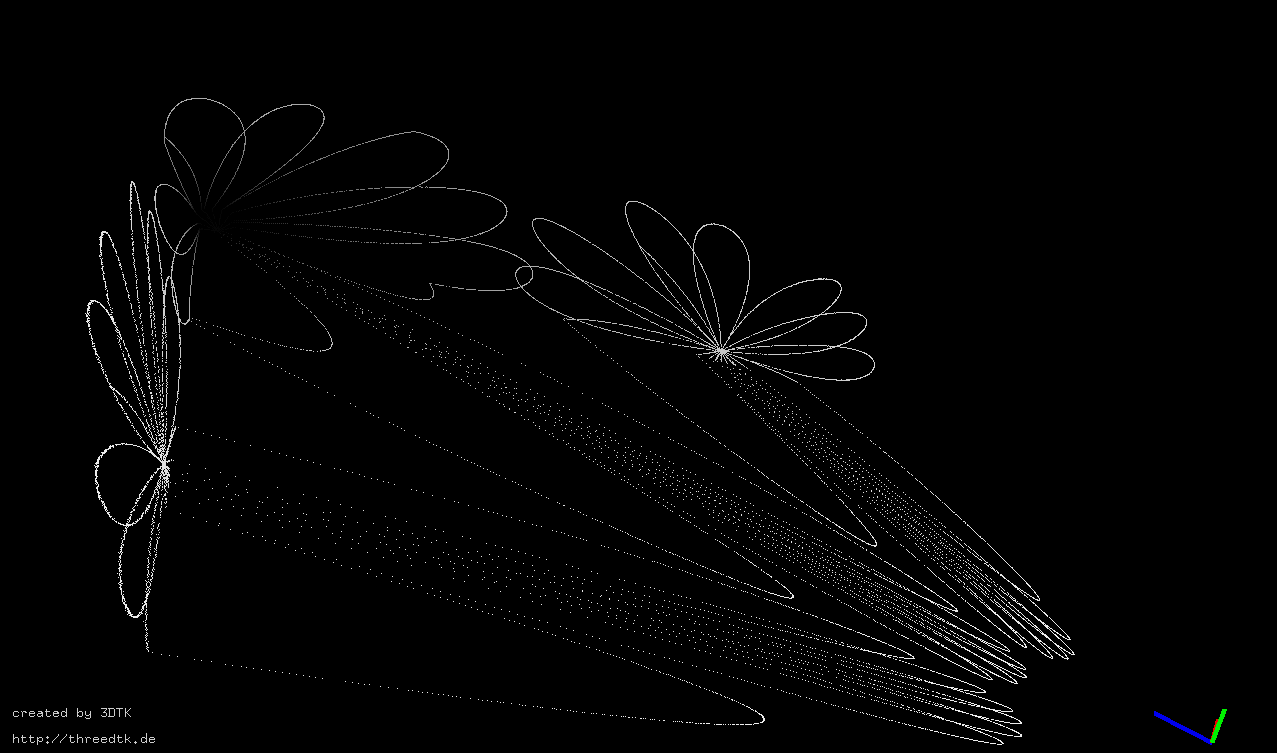
\includegraphics[width=0.495\textwidth]{images/sim_frame_00.png}\hfill
	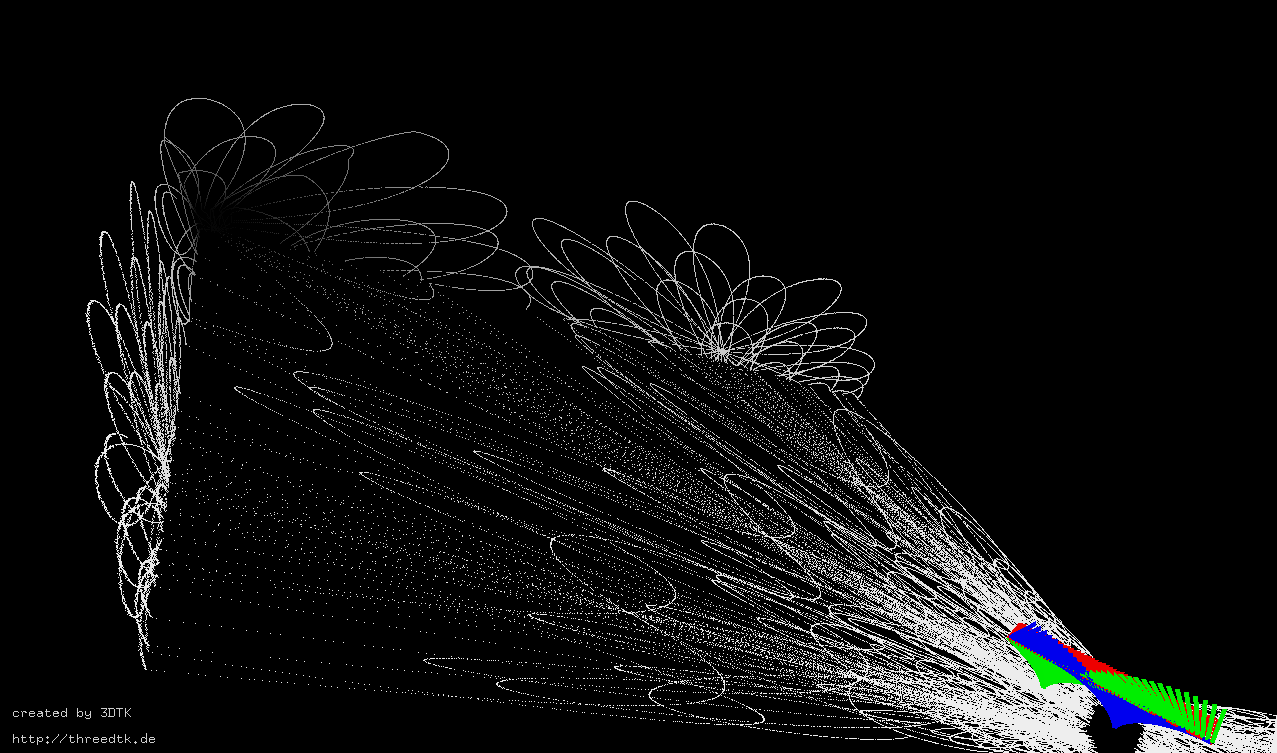
\includegraphics[width=0.495\textwidth]{images/sim_frame_02.png}\\
	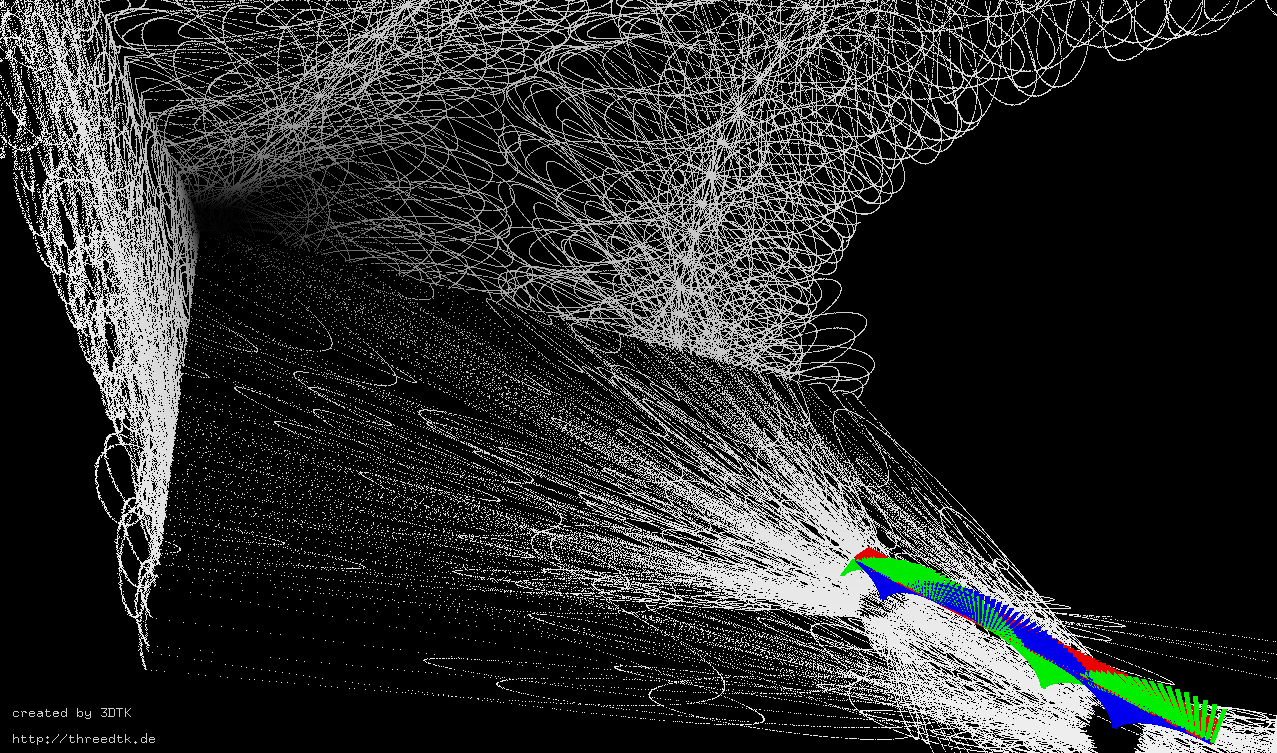
\includegraphics[width=0.495\textwidth]{images/sim_frame_06.png}\hfill
	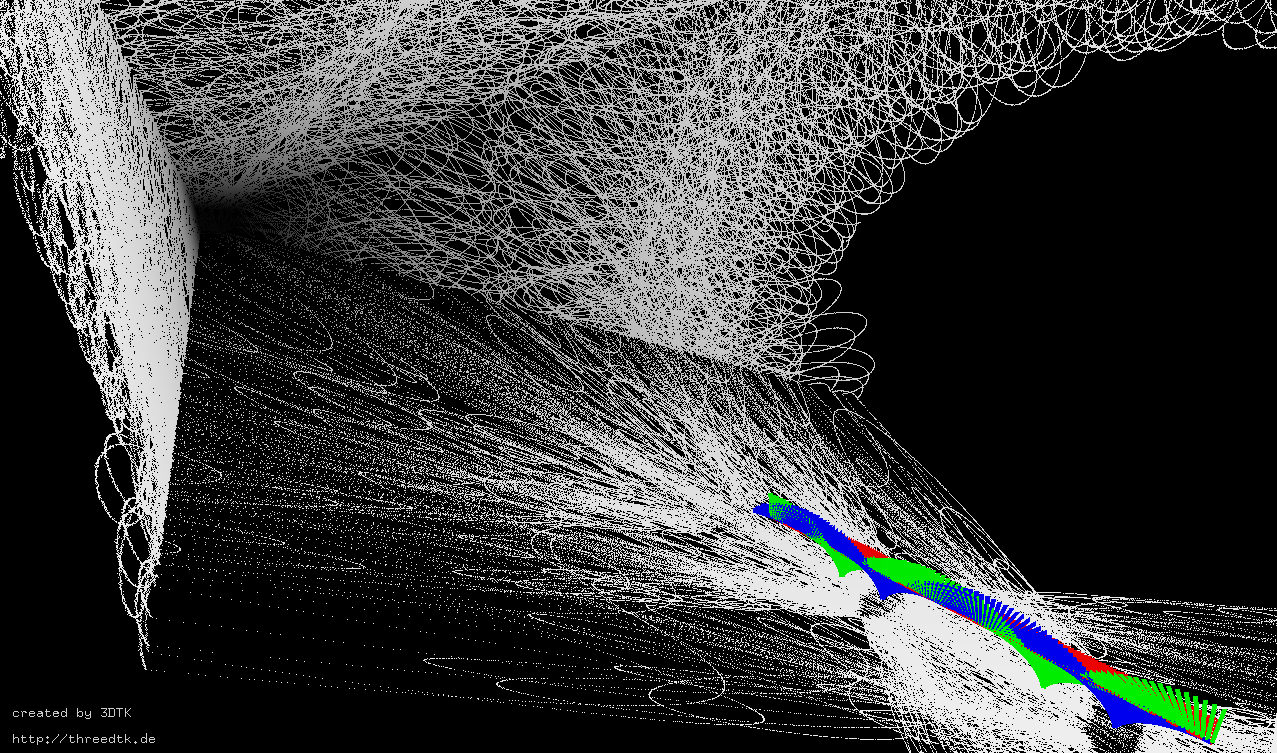
\includegraphics[width=0.495\textwidth]{images/sim_frame_08.png}\\
	\DIFdelbeginFL %DIFDELCMD < 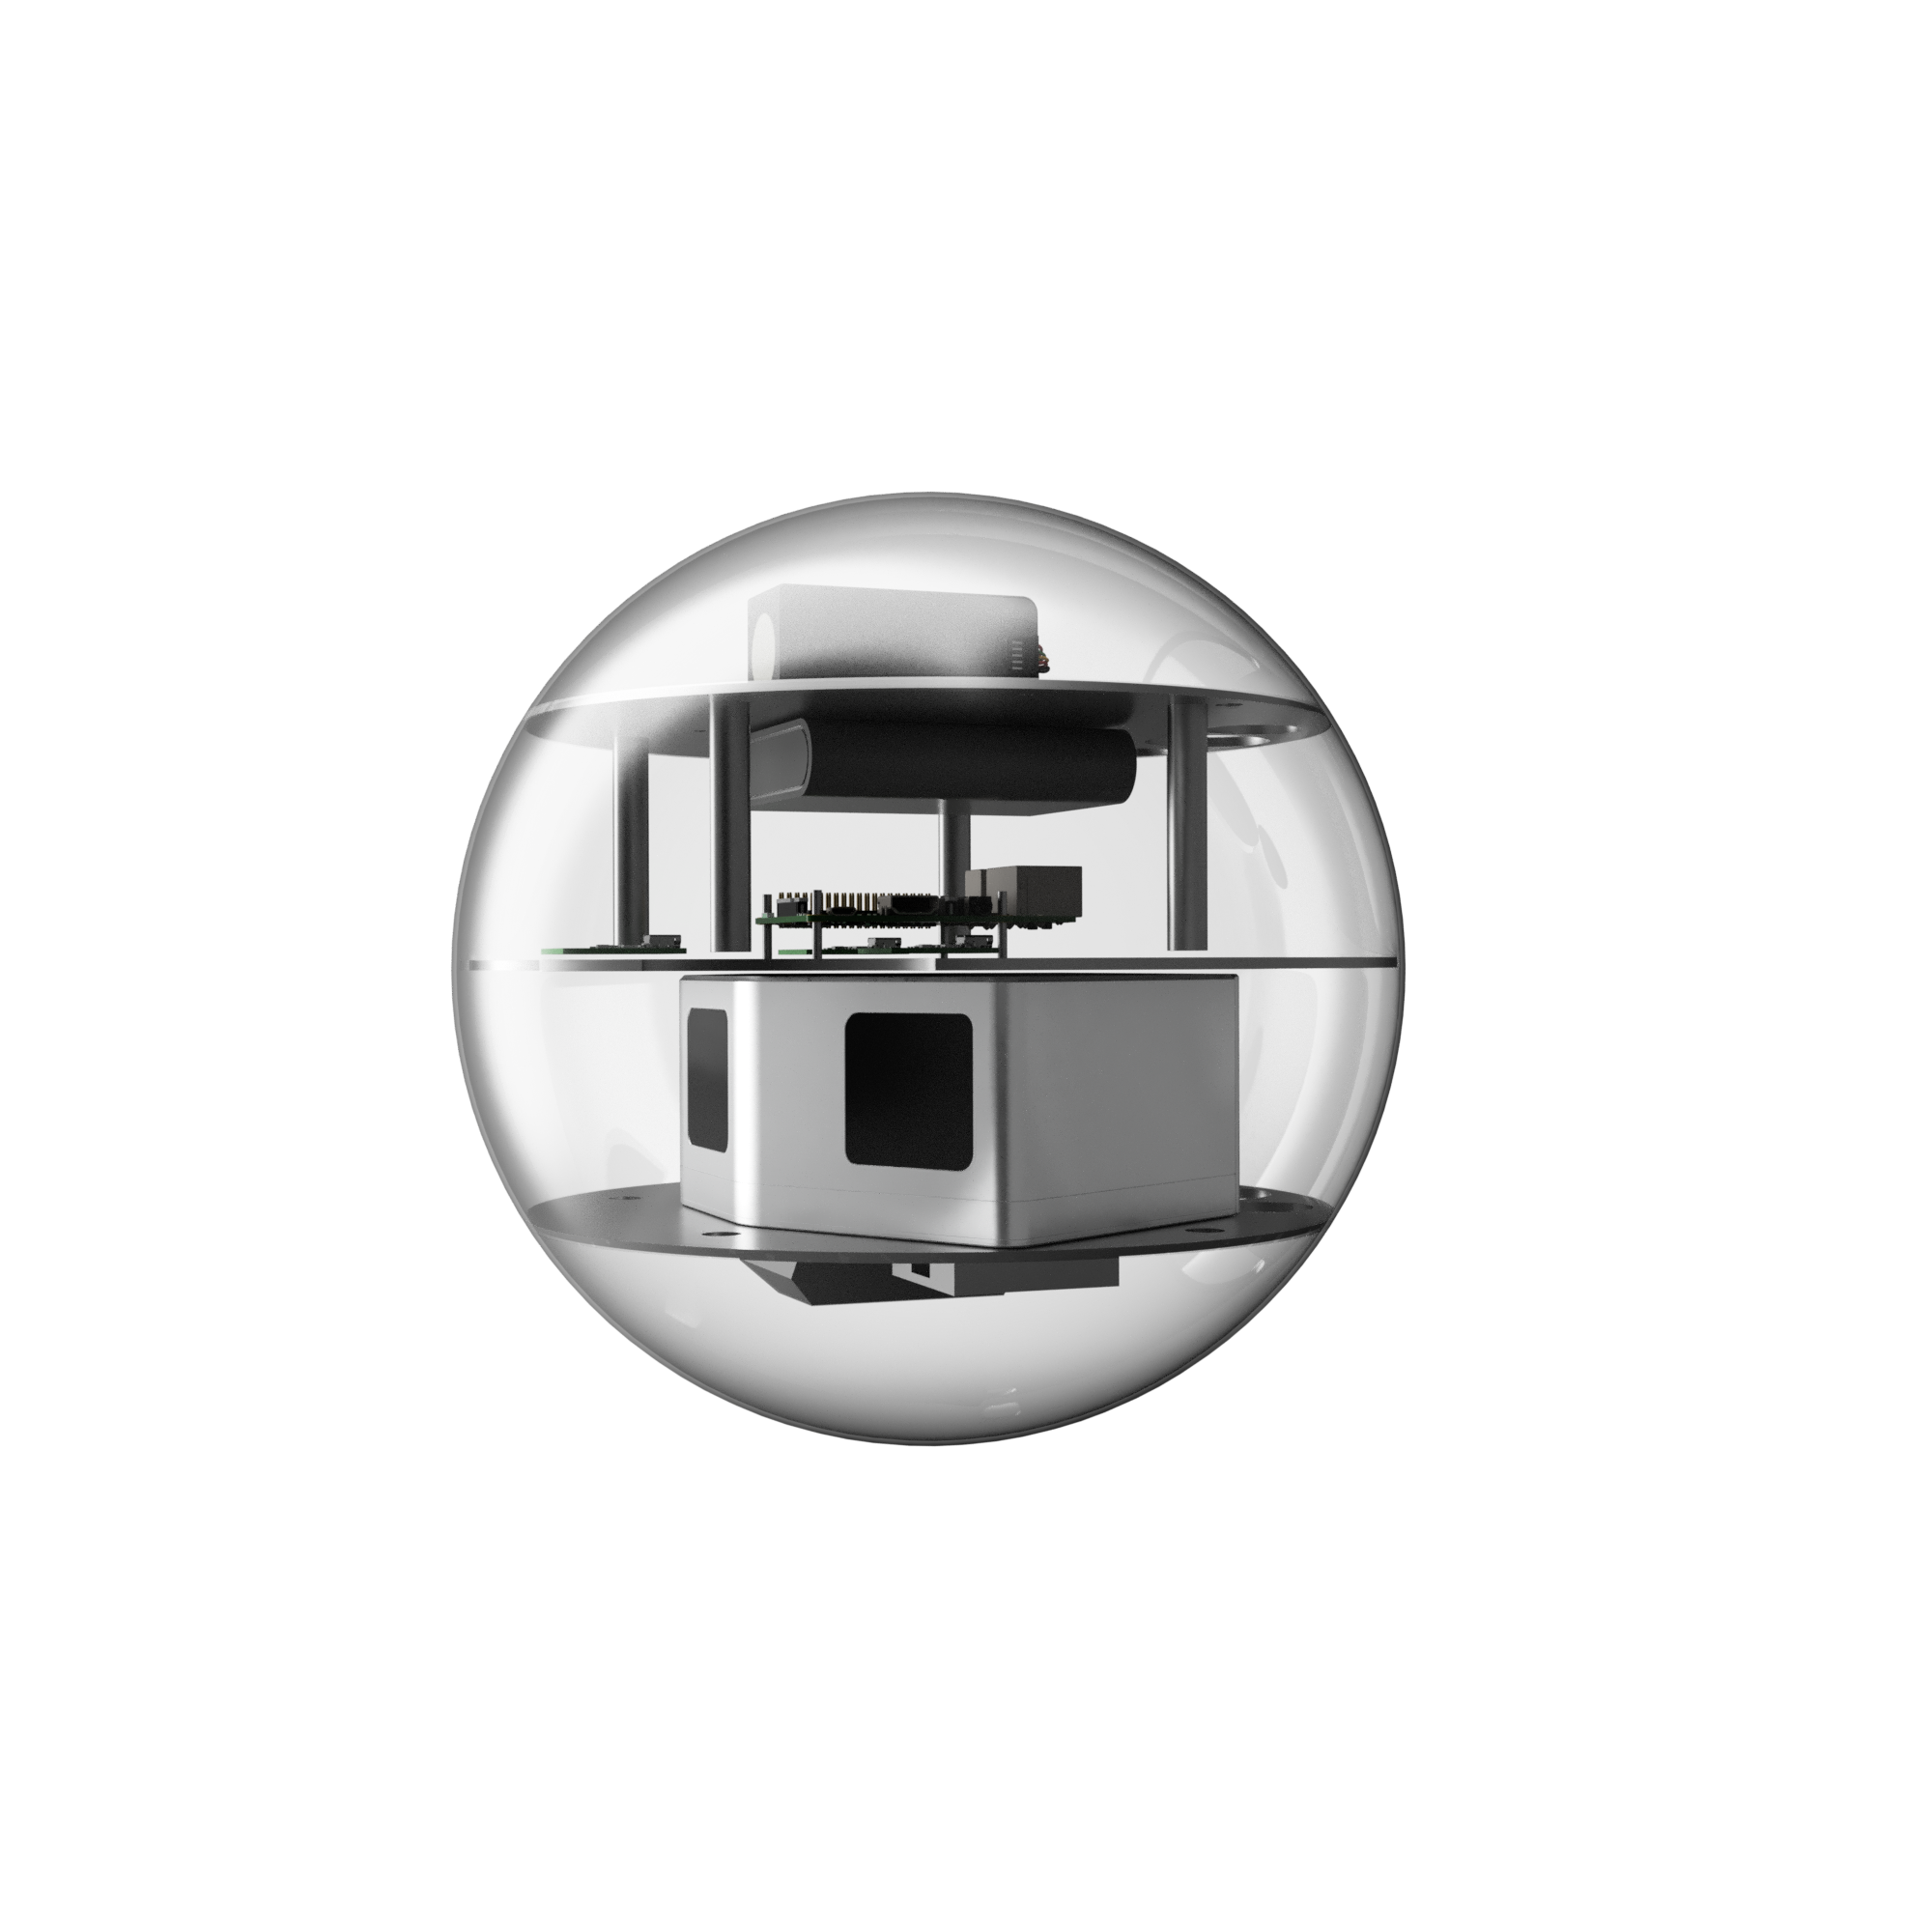
\includegraphics[width=0.495\textwidth]{images/ProtoRoll1.png}\hfill
%DIFDELCMD < 	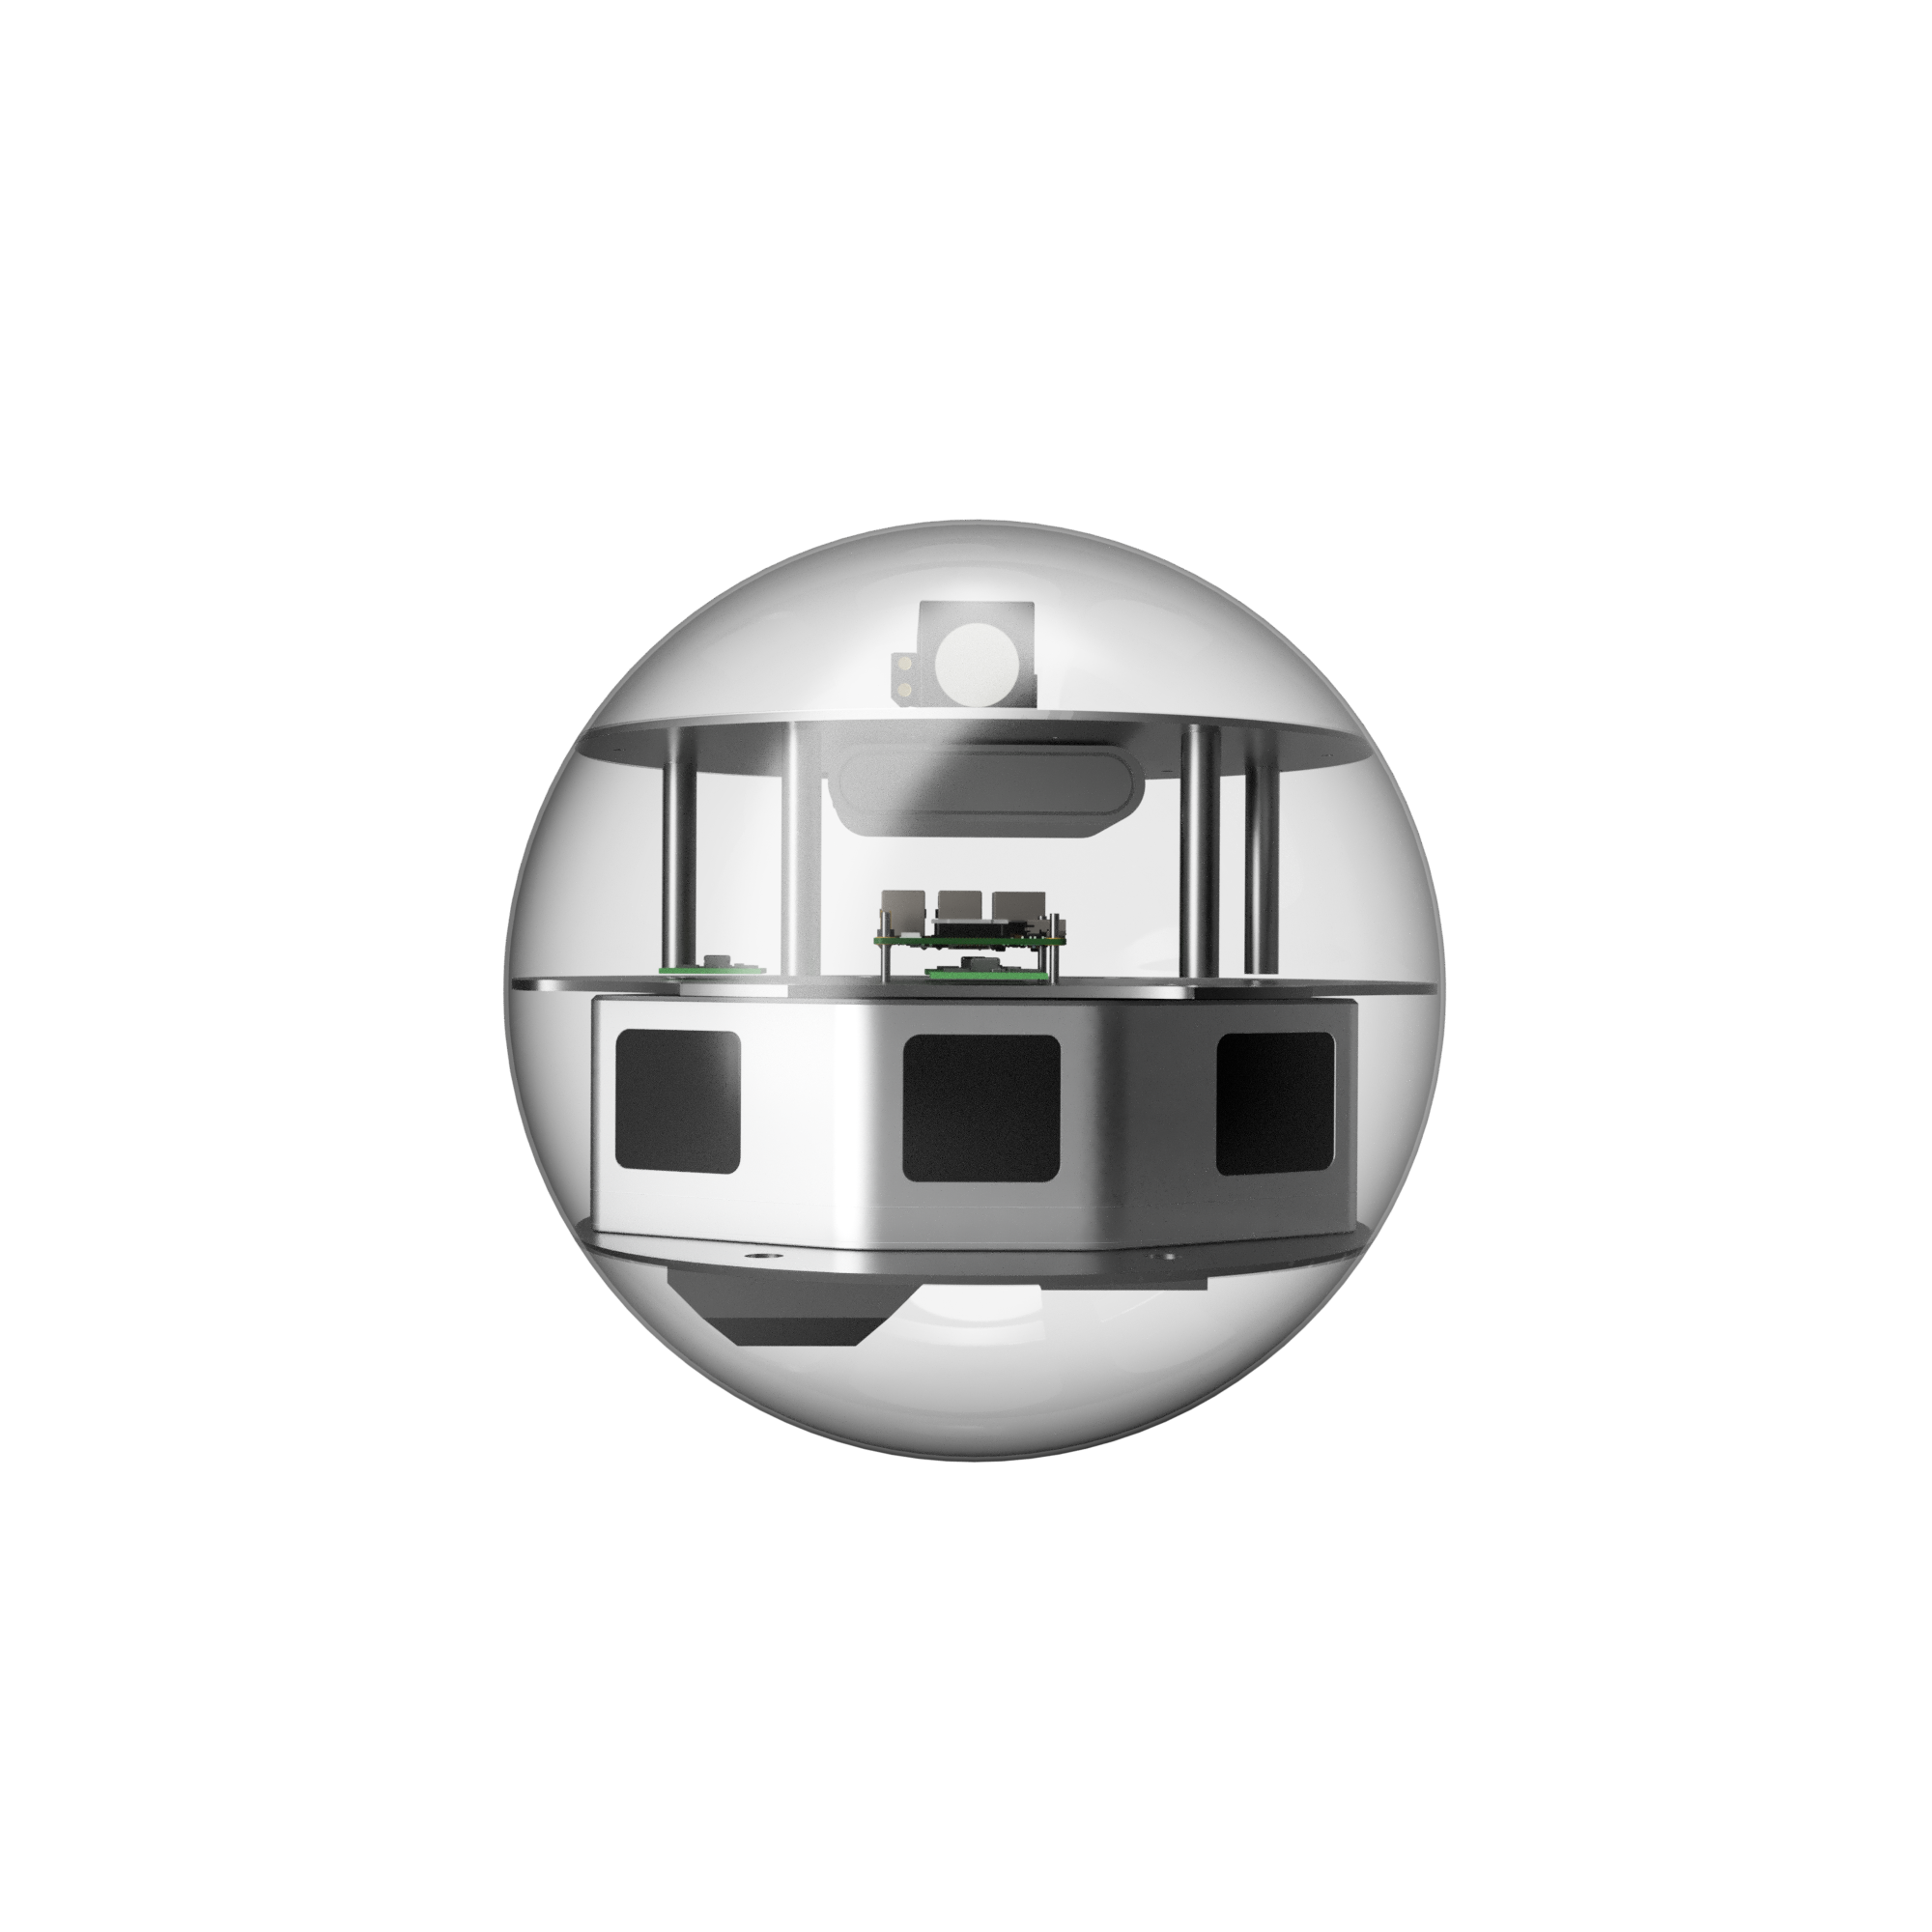
\includegraphics[width=0.495\textwidth]{images/ProtoRoll2.png}
%DIFDELCMD < 	%%%
\DIFdelendFL \caption{Top: Initial sequence of the simulation of the ideal dataset showing the simulated motion of the robot.\DIFdelbeginFL \DIFdelFL{Below: Rendering of the simulated robot, a Livox laser scanner insider a spherical shell.}\DIFdelendFL }
	\label{fig:robotRender}
\end{figure*}

%!TEX root = ../main.tex
\section{Experimental Setup}\label{sec:experimentalSetup}

We also tested \DIFdelbegin \DIFdel{out algorithm on a }\DIFdelend \DIFaddbegin \DIFadd{our algorithm on two }\DIFaddend real-world \DIFdelbegin \DIFdel{dataset that adheres }\DIFdelend \DIFaddbegin \DIFadd{datasets that adhere }\DIFaddend to different motion profiles and laser \DIFdelbegin \DIFdel{scanners type }\DIFdelend \DIFaddbegin \DIFadd{scanner types }\DIFaddend with different scanning patterns\DIFdelbegin \DIFdel{than the simulated data}\DIFdelend .

The \DIFaddbegin \DIFadd{first }\DIFaddend dataset is collected by a line scanner, in particular a SICK LMS141 industrial scanner, inside a sphere of a diameter of \SI{20}{\centi\meter} that lies on a floating desk, which is air-pressurized, such that the sphere is hovering.
On this floating desk, the sphere can rotate freely about all axis while being fixed in position. 
Hence, in this experiment the optimization space can be reduced to a rotation.
Further, without the motion, the 2D laser cannot obtain a 3D model from the environment, thus requiring registration. 
The sphere is equipped with a low-cost IMU, i.e., a PhidgetSpatial Precision 3/3/3, to estimate the orientation, a battery pack and a raspberry pie for processing.
\DIFdelbegin %DIFDELCMD < 

%DIFDELCMD < %%%
\DIFdelend \DIFaddbegin \DIFadd{This IMU provides a precision of \mbox{%DIFAUXCMD
\SI{76.3}{\micro g} }\hspace{0pt}%DIFAUXCMD
in linear acceleration, \mbox{%DIFAUXCMD
\SI{0.02}{\degree\per\second} }\hspace{0pt}%DIFAUXCMD
in angular velocity about the x and y axis, and \mbox{%DIFAUXCMD
\SI{0.013}{\degree\per\second} }\hspace{0pt}%DIFAUXCMD
in angular velocity about the z axis \mbox{%DIFAUXCMD
\cite{PhidgetSpatial}}\hspace{0pt}%DIFAUXCMD
.  
}\DIFaddend Figure~\ref{fig:float-sat-sphere} shows the experimental setup. The left column of figure~\ref{fig:cylon-corrected} shows the pre-registered resulting point cloud. 
We see that the point cloud is rather noisy, and in particular, the walls are sensed multiple times, hence appearing very blurry. 

\begin{figure}
	\centering
	\begin{minipage}[c]{0.45\textwidth}
		\centering
		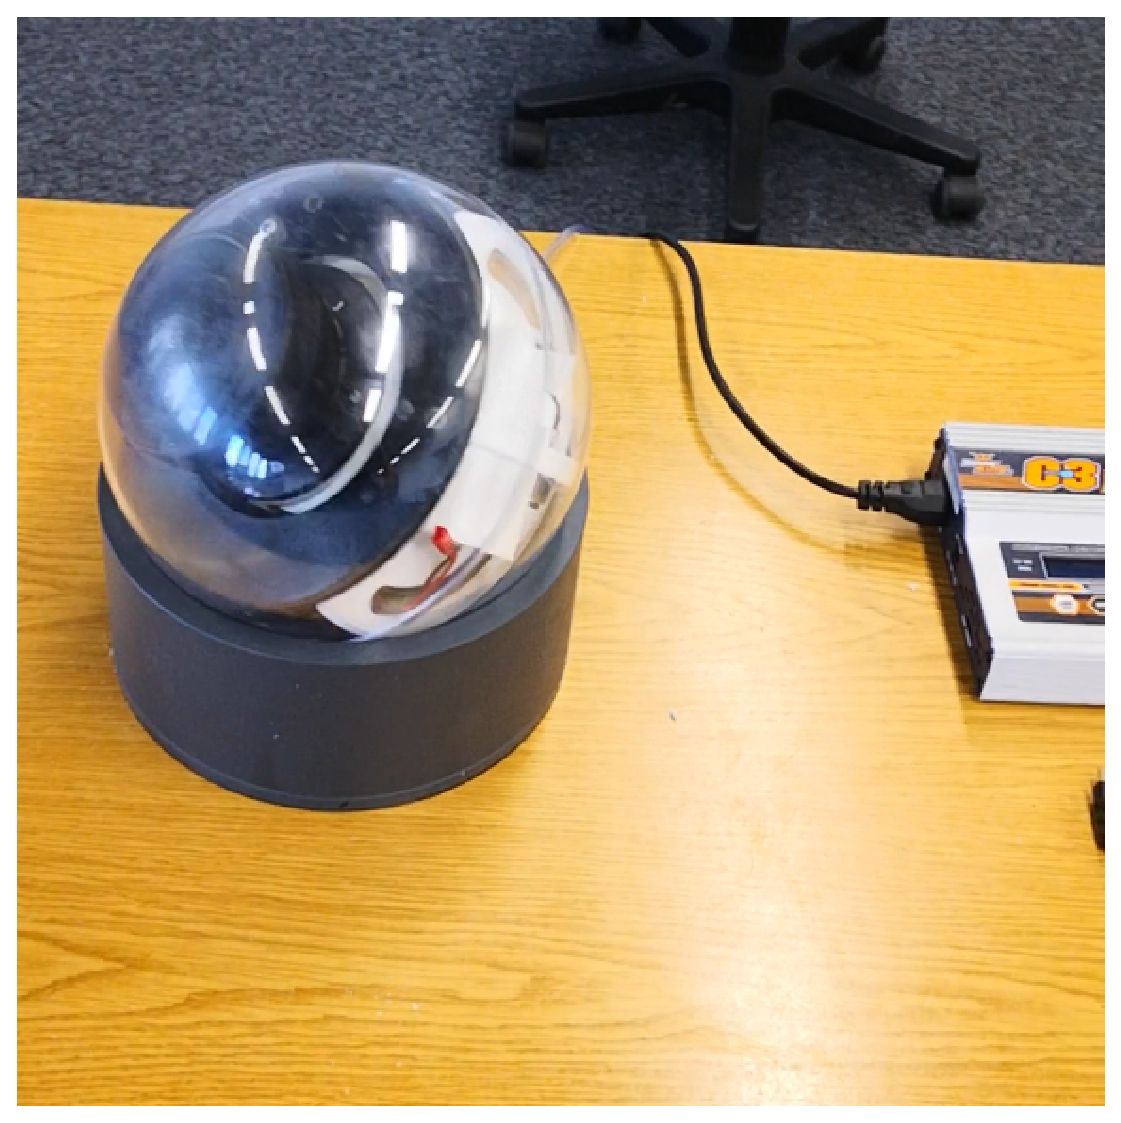
\includegraphics[width=0.33\textwidth, height=0.33\textwidth]{./images/sphere-frame-1.eps}\hfill
		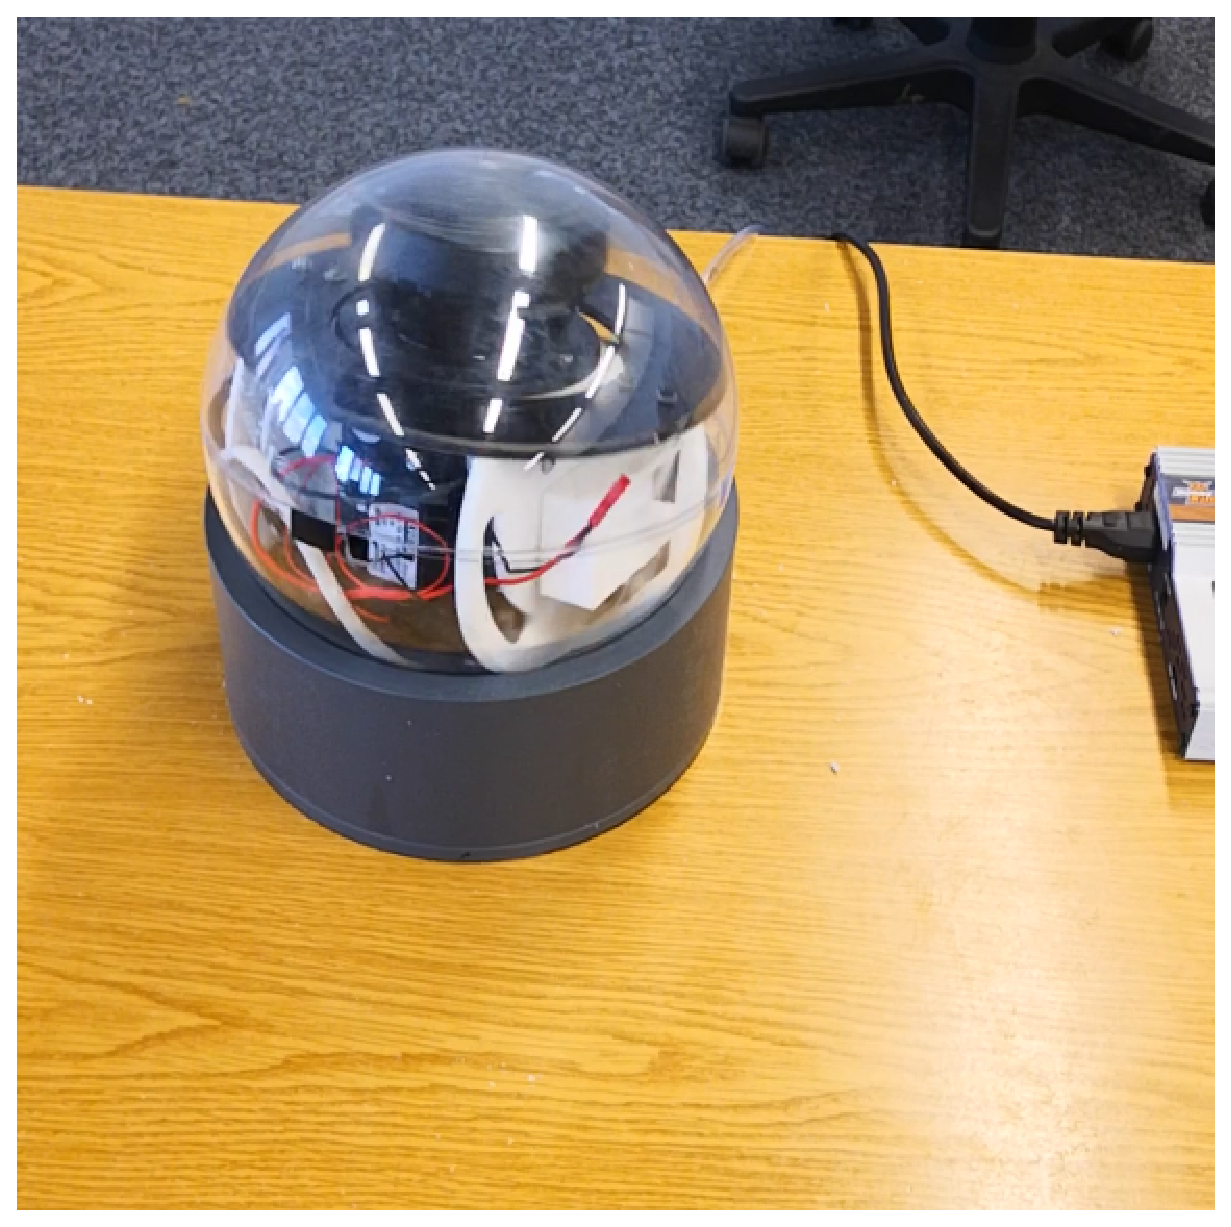
\includegraphics[width=0.33\textwidth, height=0.33\textwidth]{./images/sphere-frame-2.eps}\hfill
		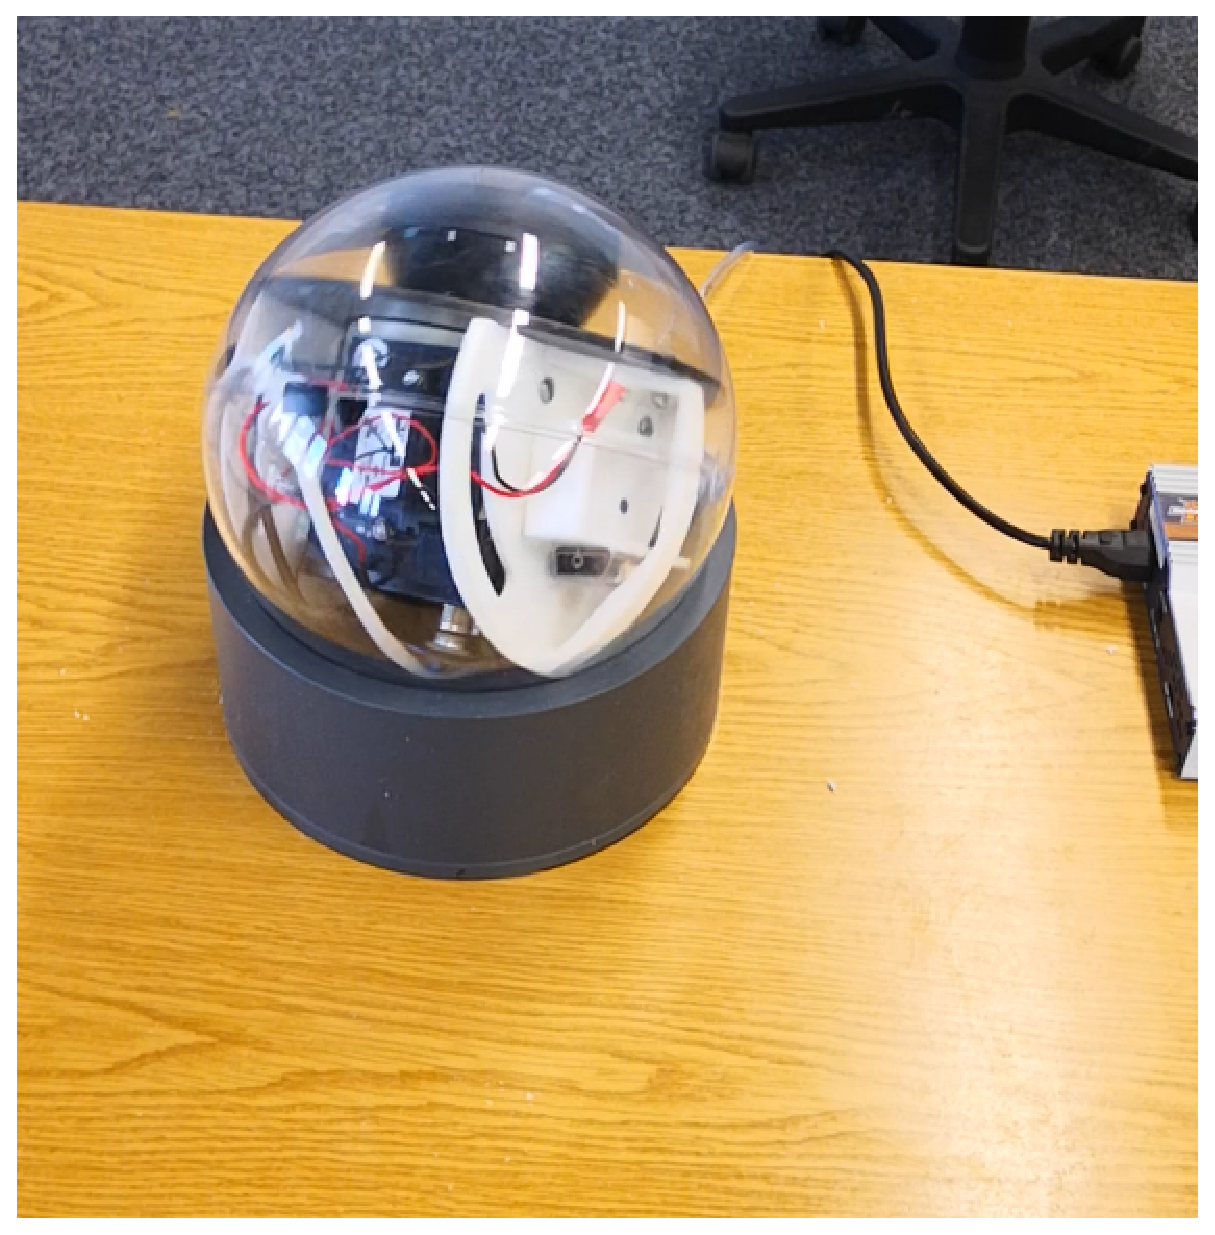
\includegraphics[width=0.33\textwidth, height=0.33\textwidth]{./images/sphere-frame-3.eps}\\
		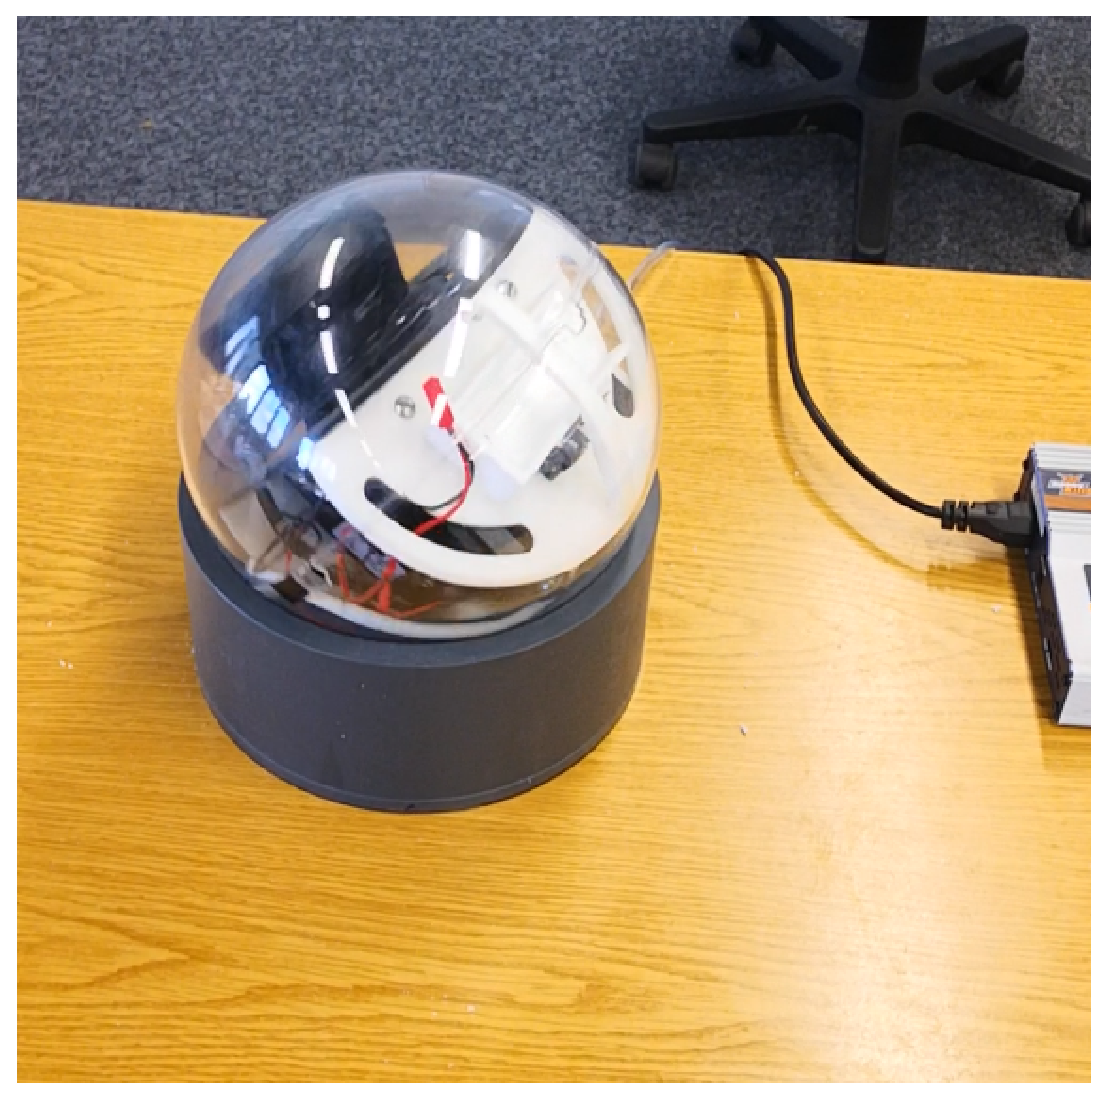
\includegraphics[width=0.33\textwidth, height=0.33\textwidth]{./images/sphere-frame-4.eps}\hfill
		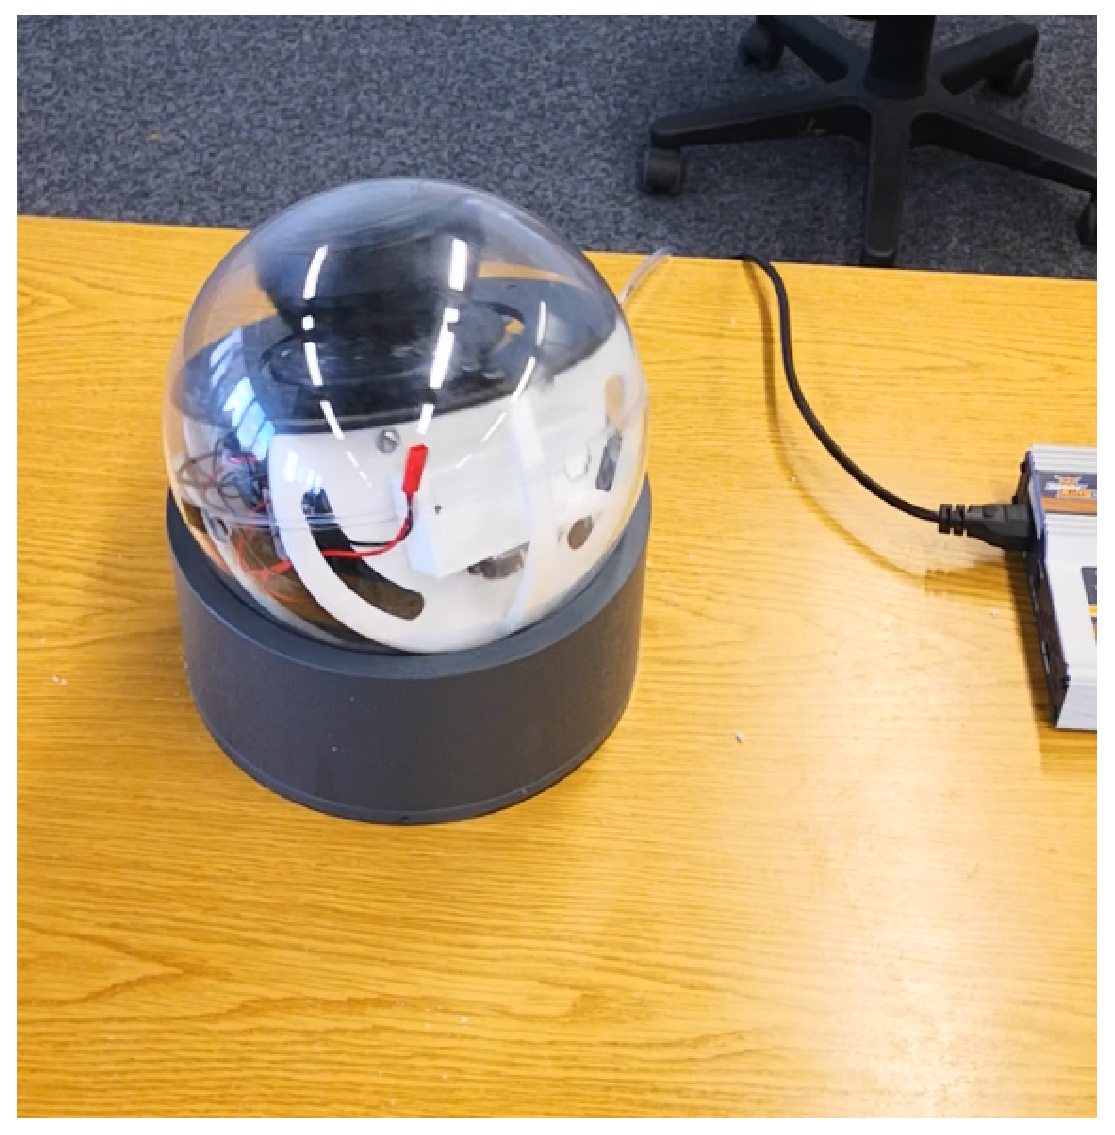
\includegraphics[width=0.33\textwidth, height=0.33\textwidth]{./images/sphere-frame-5.eps}\hfill
		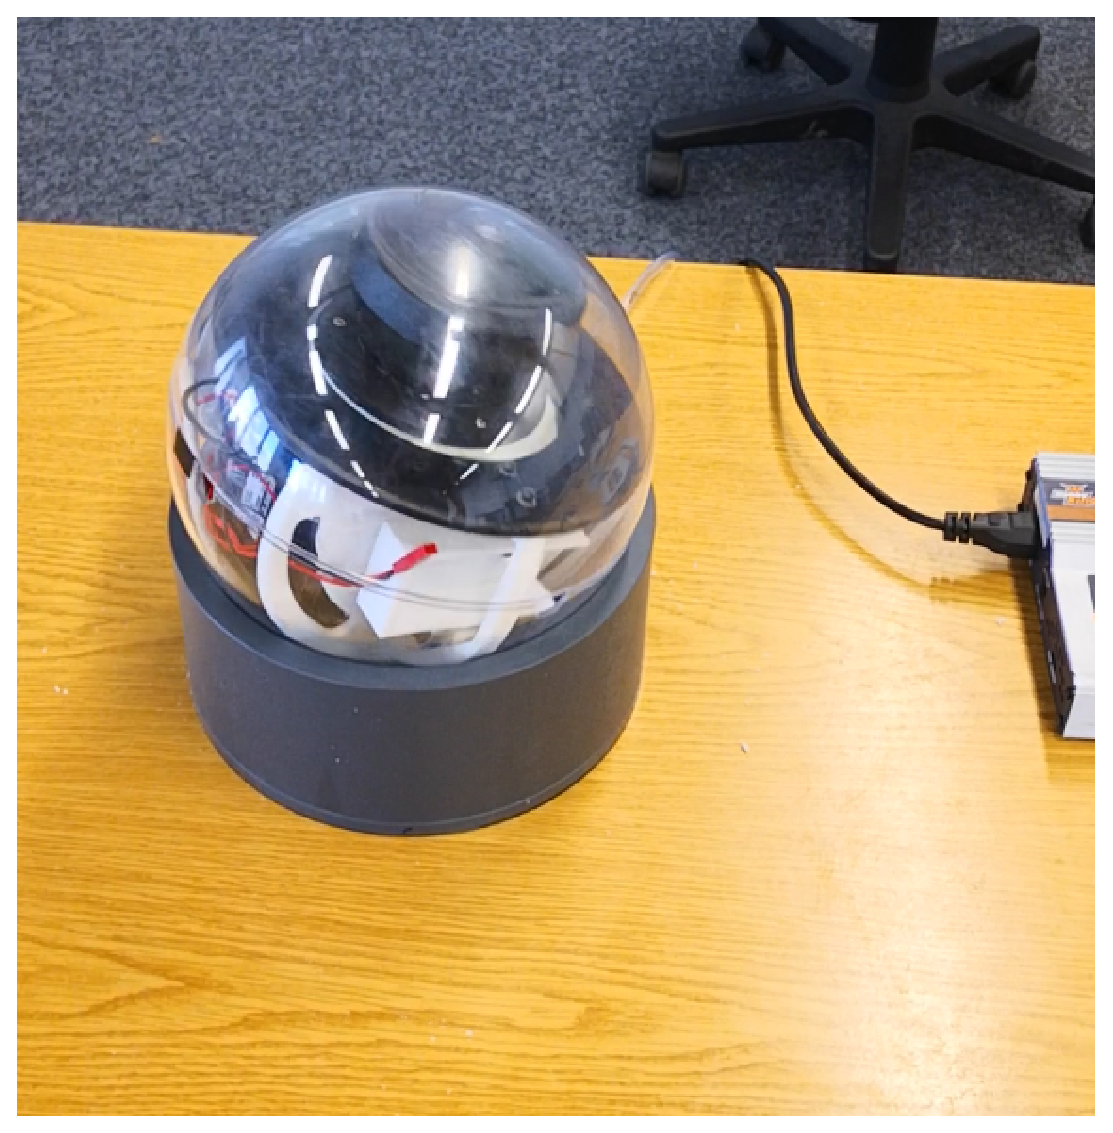
\includegraphics[width=0.33\textwidth, height=0.33\textwidth]{./images/sphere-frame-6.eps}\hfill
	\end{minipage}\\
	\vspace{0.1cm}
	\begin{minipage}[c]{0.45\textwidth}
		\centering
		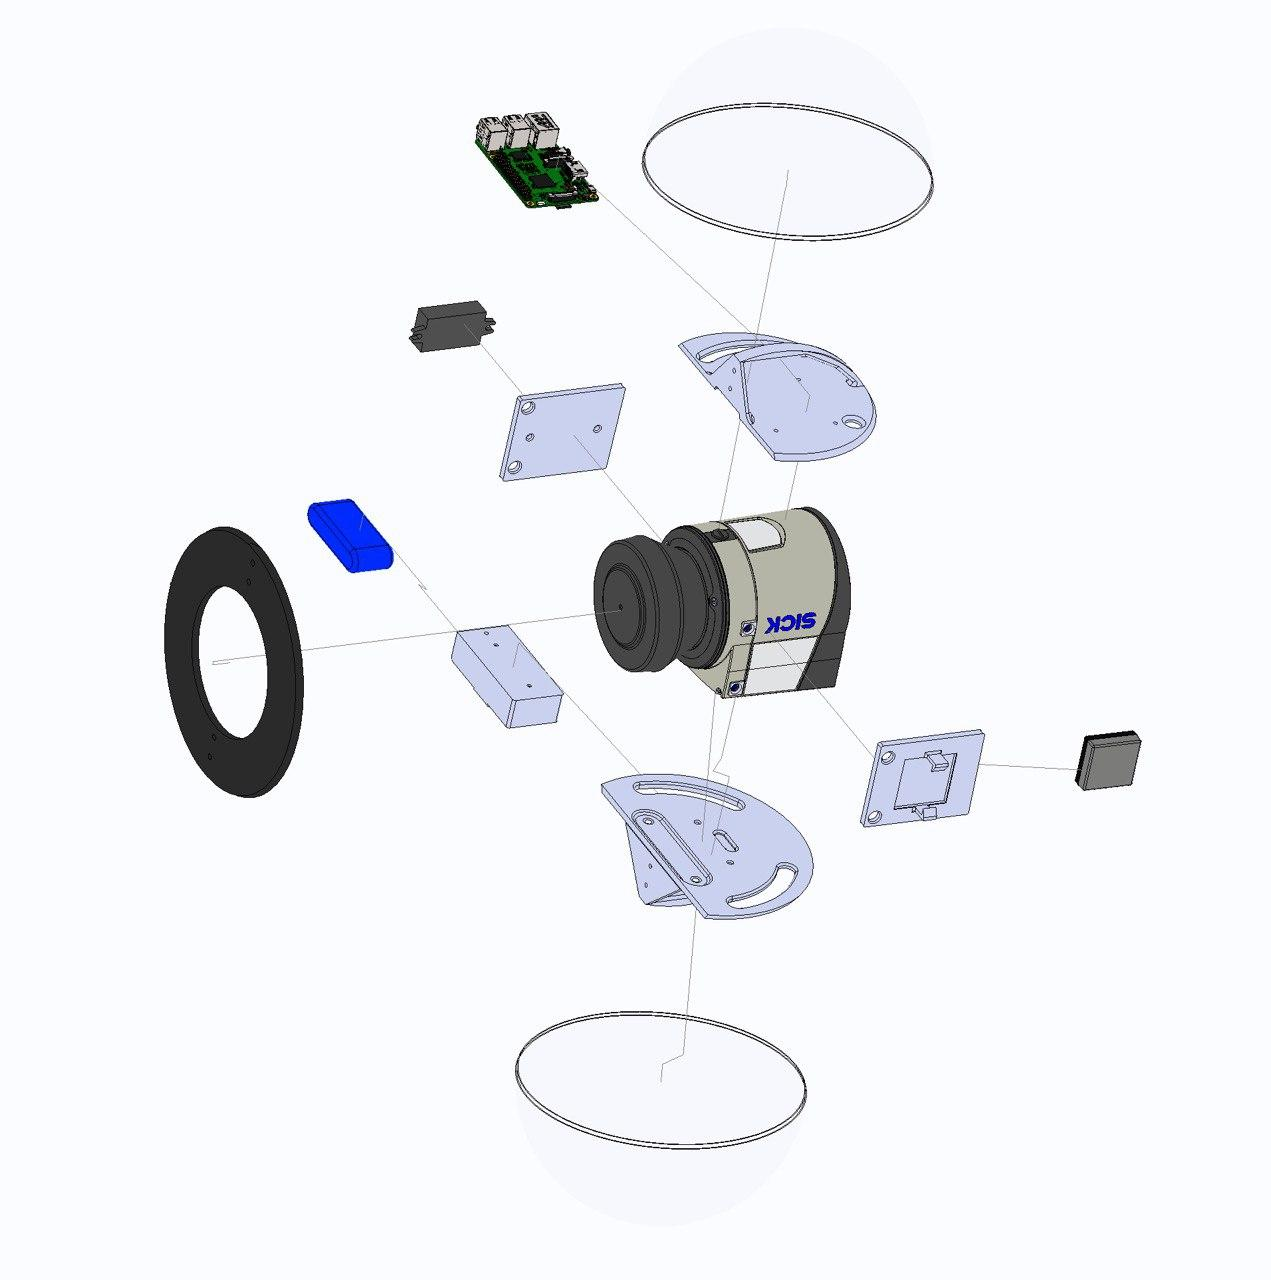
\includegraphics[width=0.495\textwidth]{./images/cylon_exploded}\hfill
		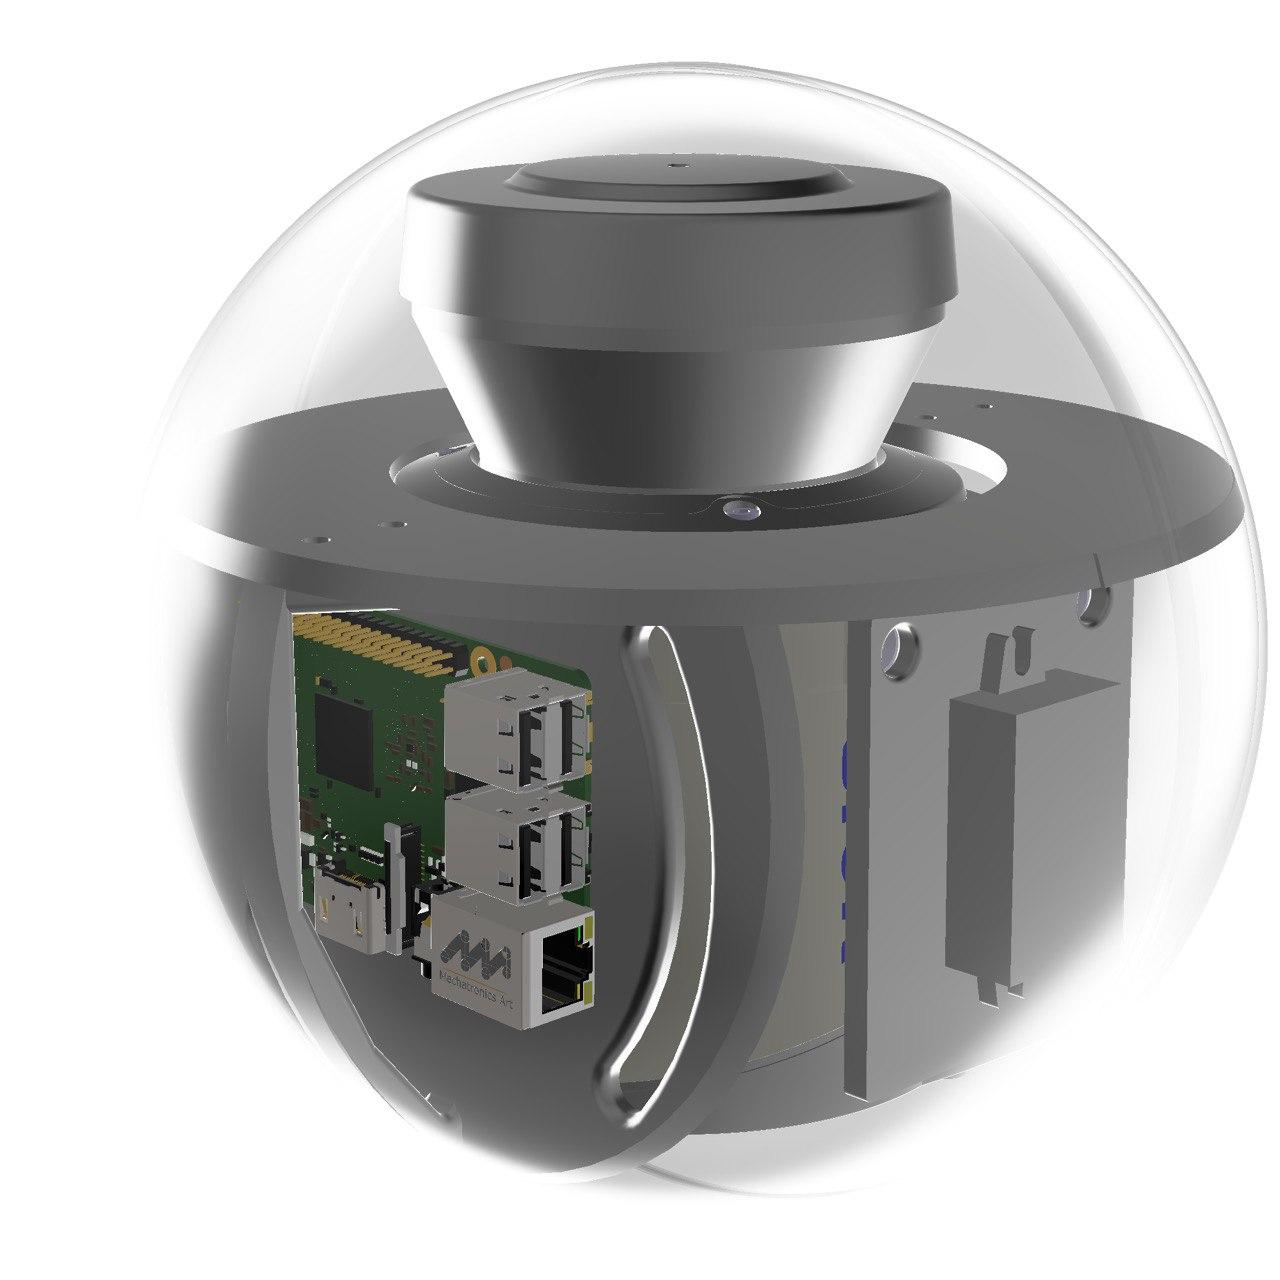
\includegraphics[width=0.495\textwidth]{./images/cylon_setup}\hfill
	\end{minipage}
	\caption{Data acquisition using floating sphere. Top: A sequence of orientations the sphere assumes during data acquisition. Bottom: Hardware setup of the sphere.} 
	\label{fig:float-sat-sphere}
\end{figure}

\DIFaddbegin \DIFadd{The second datasets is collected by a 3D scanner, namely the LIVOX MID 100, which is the same sensor the simulation uses.
We put the laser scanner into an acrylic glass spherical shell together with three IMUs  (same specifications as in the first dataset) and manually roll it with a slow, constant motion in a home indoor environment.
Thus, this time nearly all six degrees of freedom are used for optimization.
We exclude a translation in the global up- or downwards direction as the sphere rolls on the ground surface, without possibility for up- or downwards motion-
Figure~\ref{fig:prototype} shows the prototype.
The left column of figure~\ref{fig:jasperhome} shows the pre-registered point cloud, applying only the transformation defined by the recorded poses.
Although the robot has been moved carefully, you see that pose error accumulates in such a way that the same wall is sensed multiple times.   
}

\begin{figure}
  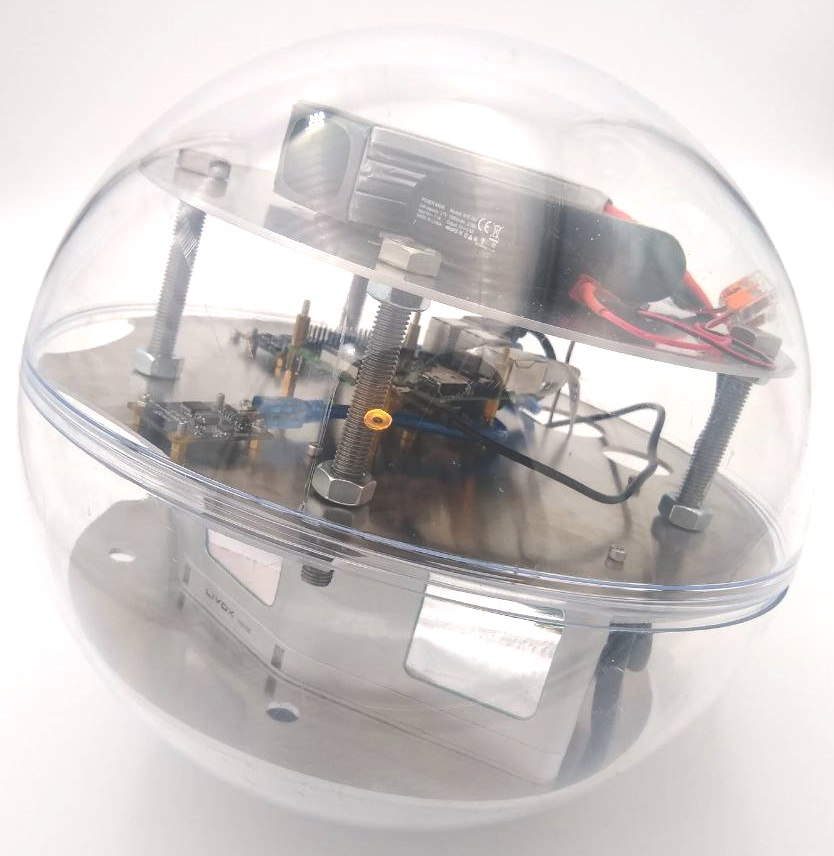
\includegraphics[width=0.495\linewidth]{./images/photoReal1.jpeg}\hfill
  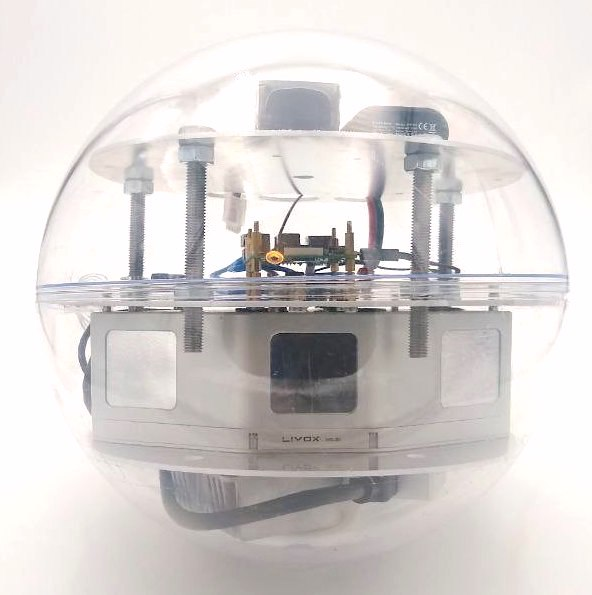
\includegraphics[width=0.495\linewidth]{./images/photoReal3.jpeg}\\
  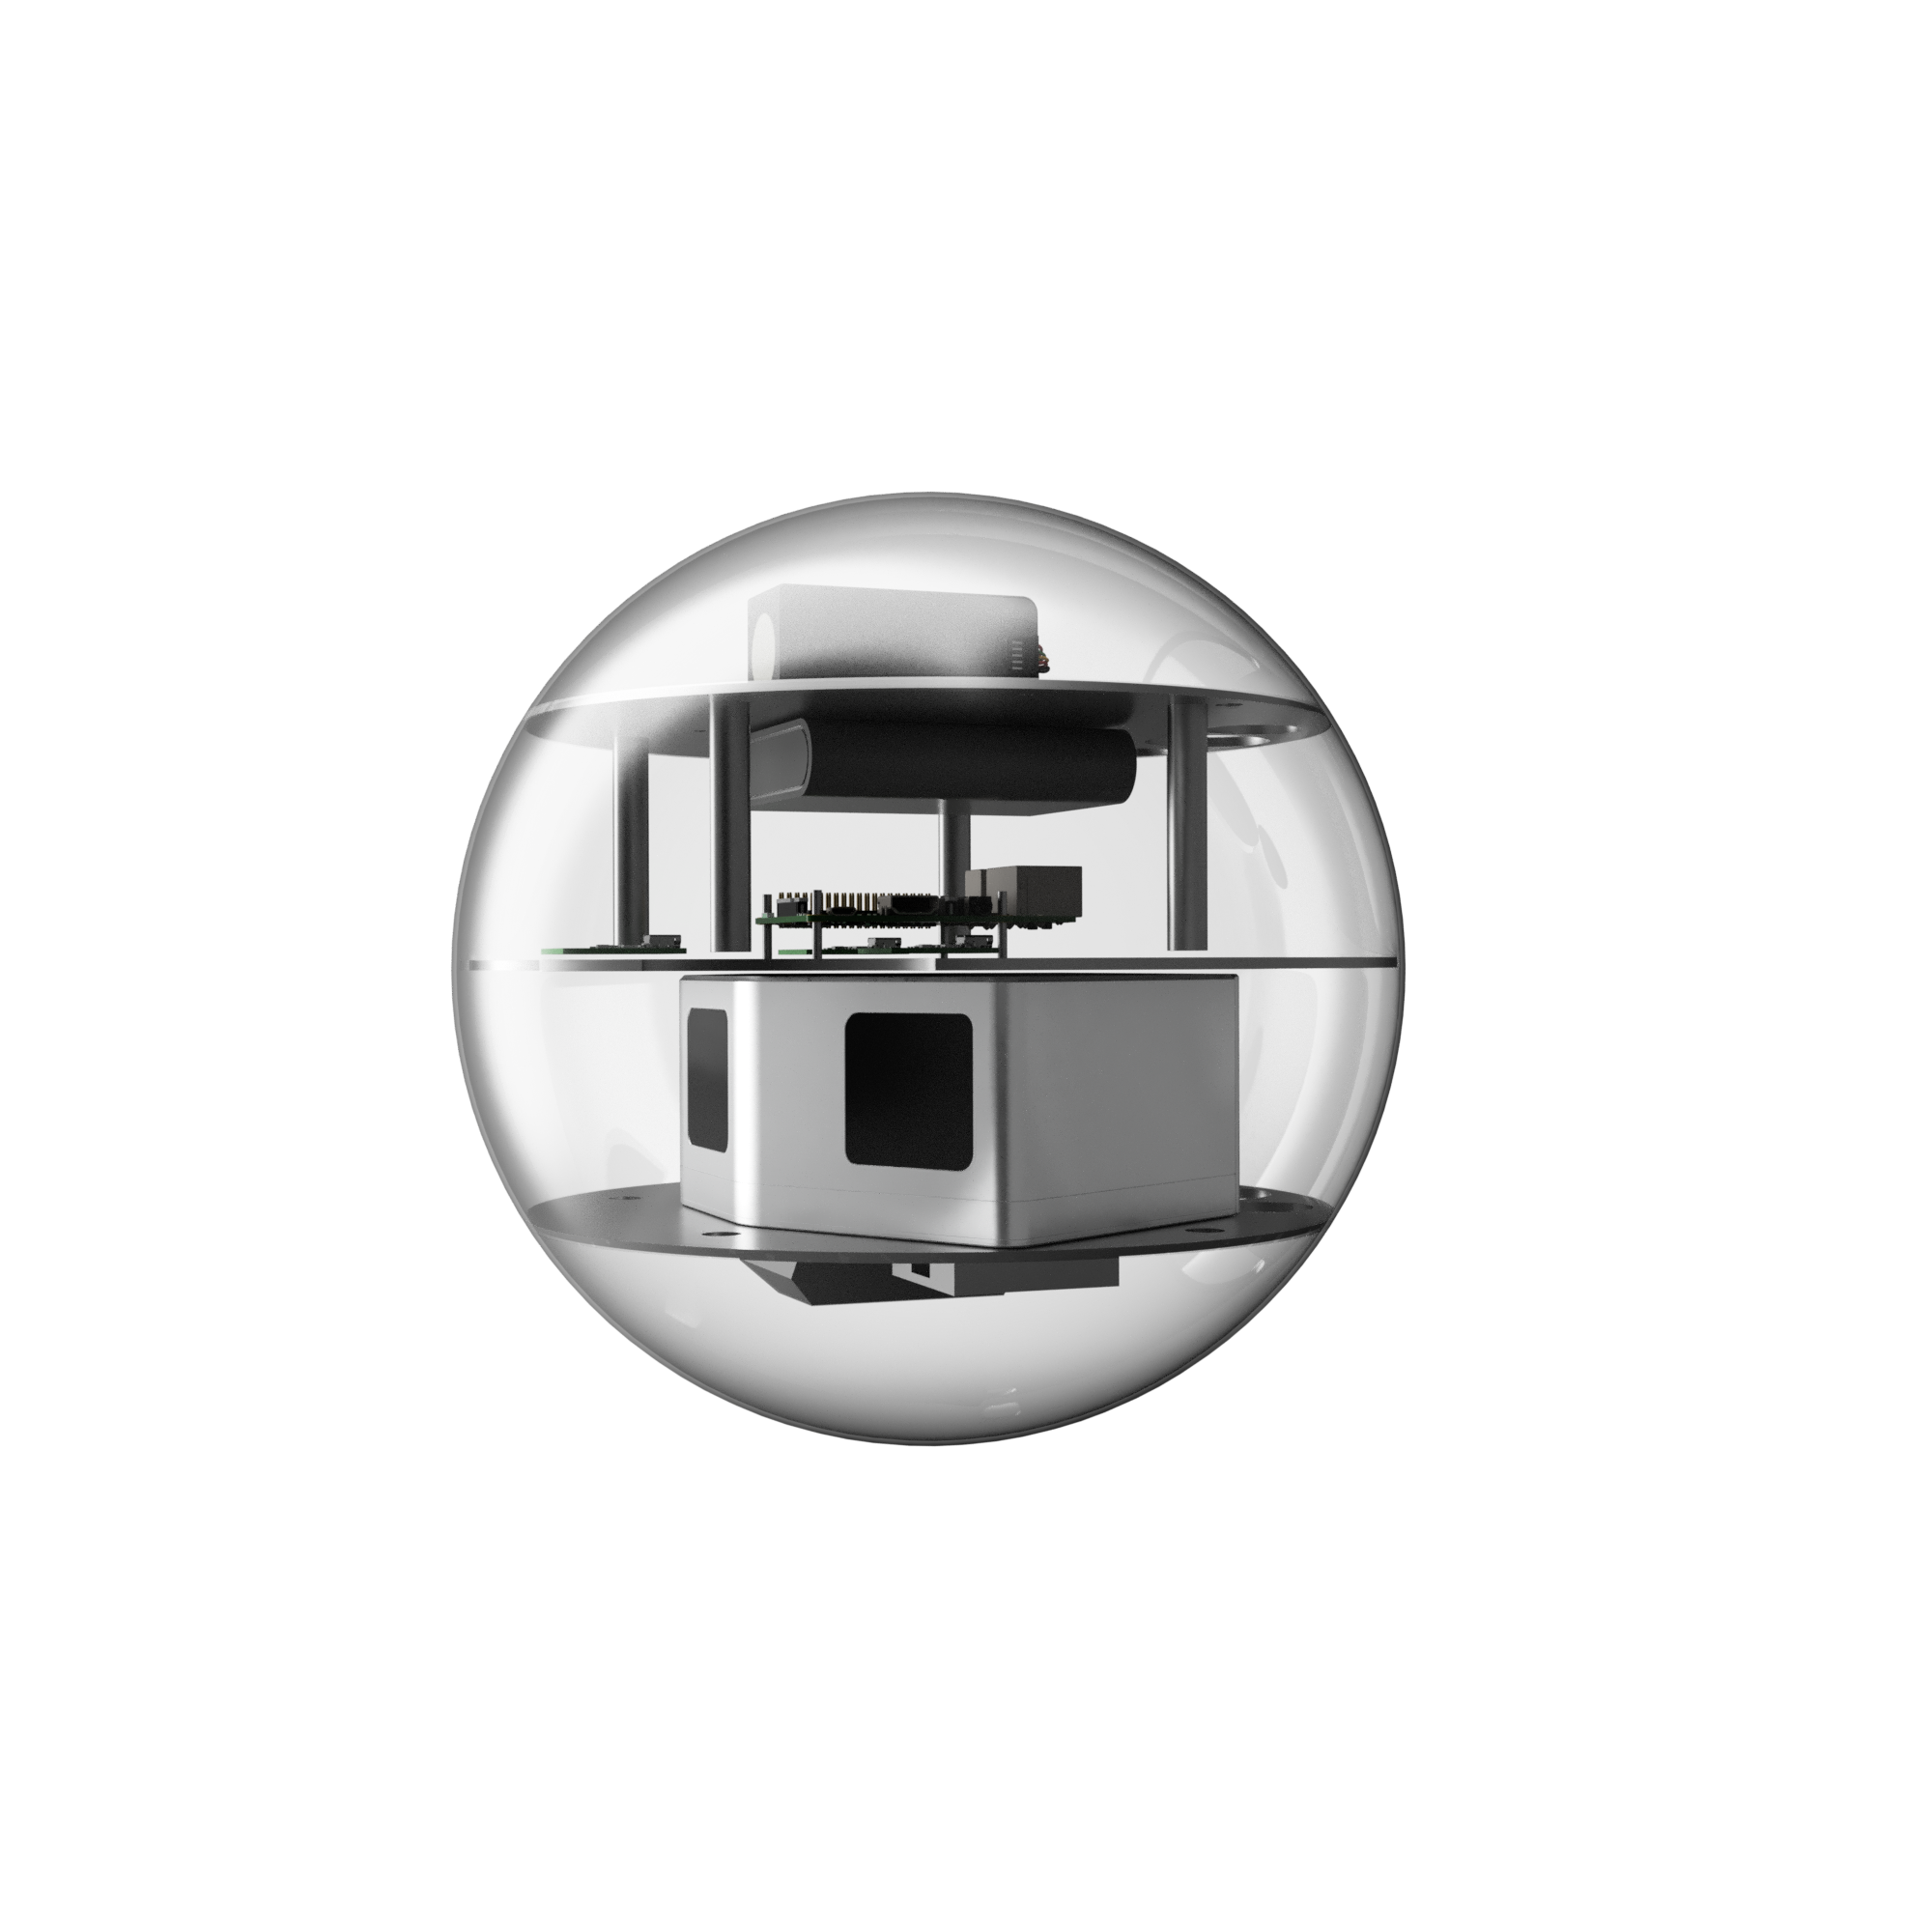
\includegraphics[width=0.495\linewidth]{./images/ProtoRoll1.png}\hfill
  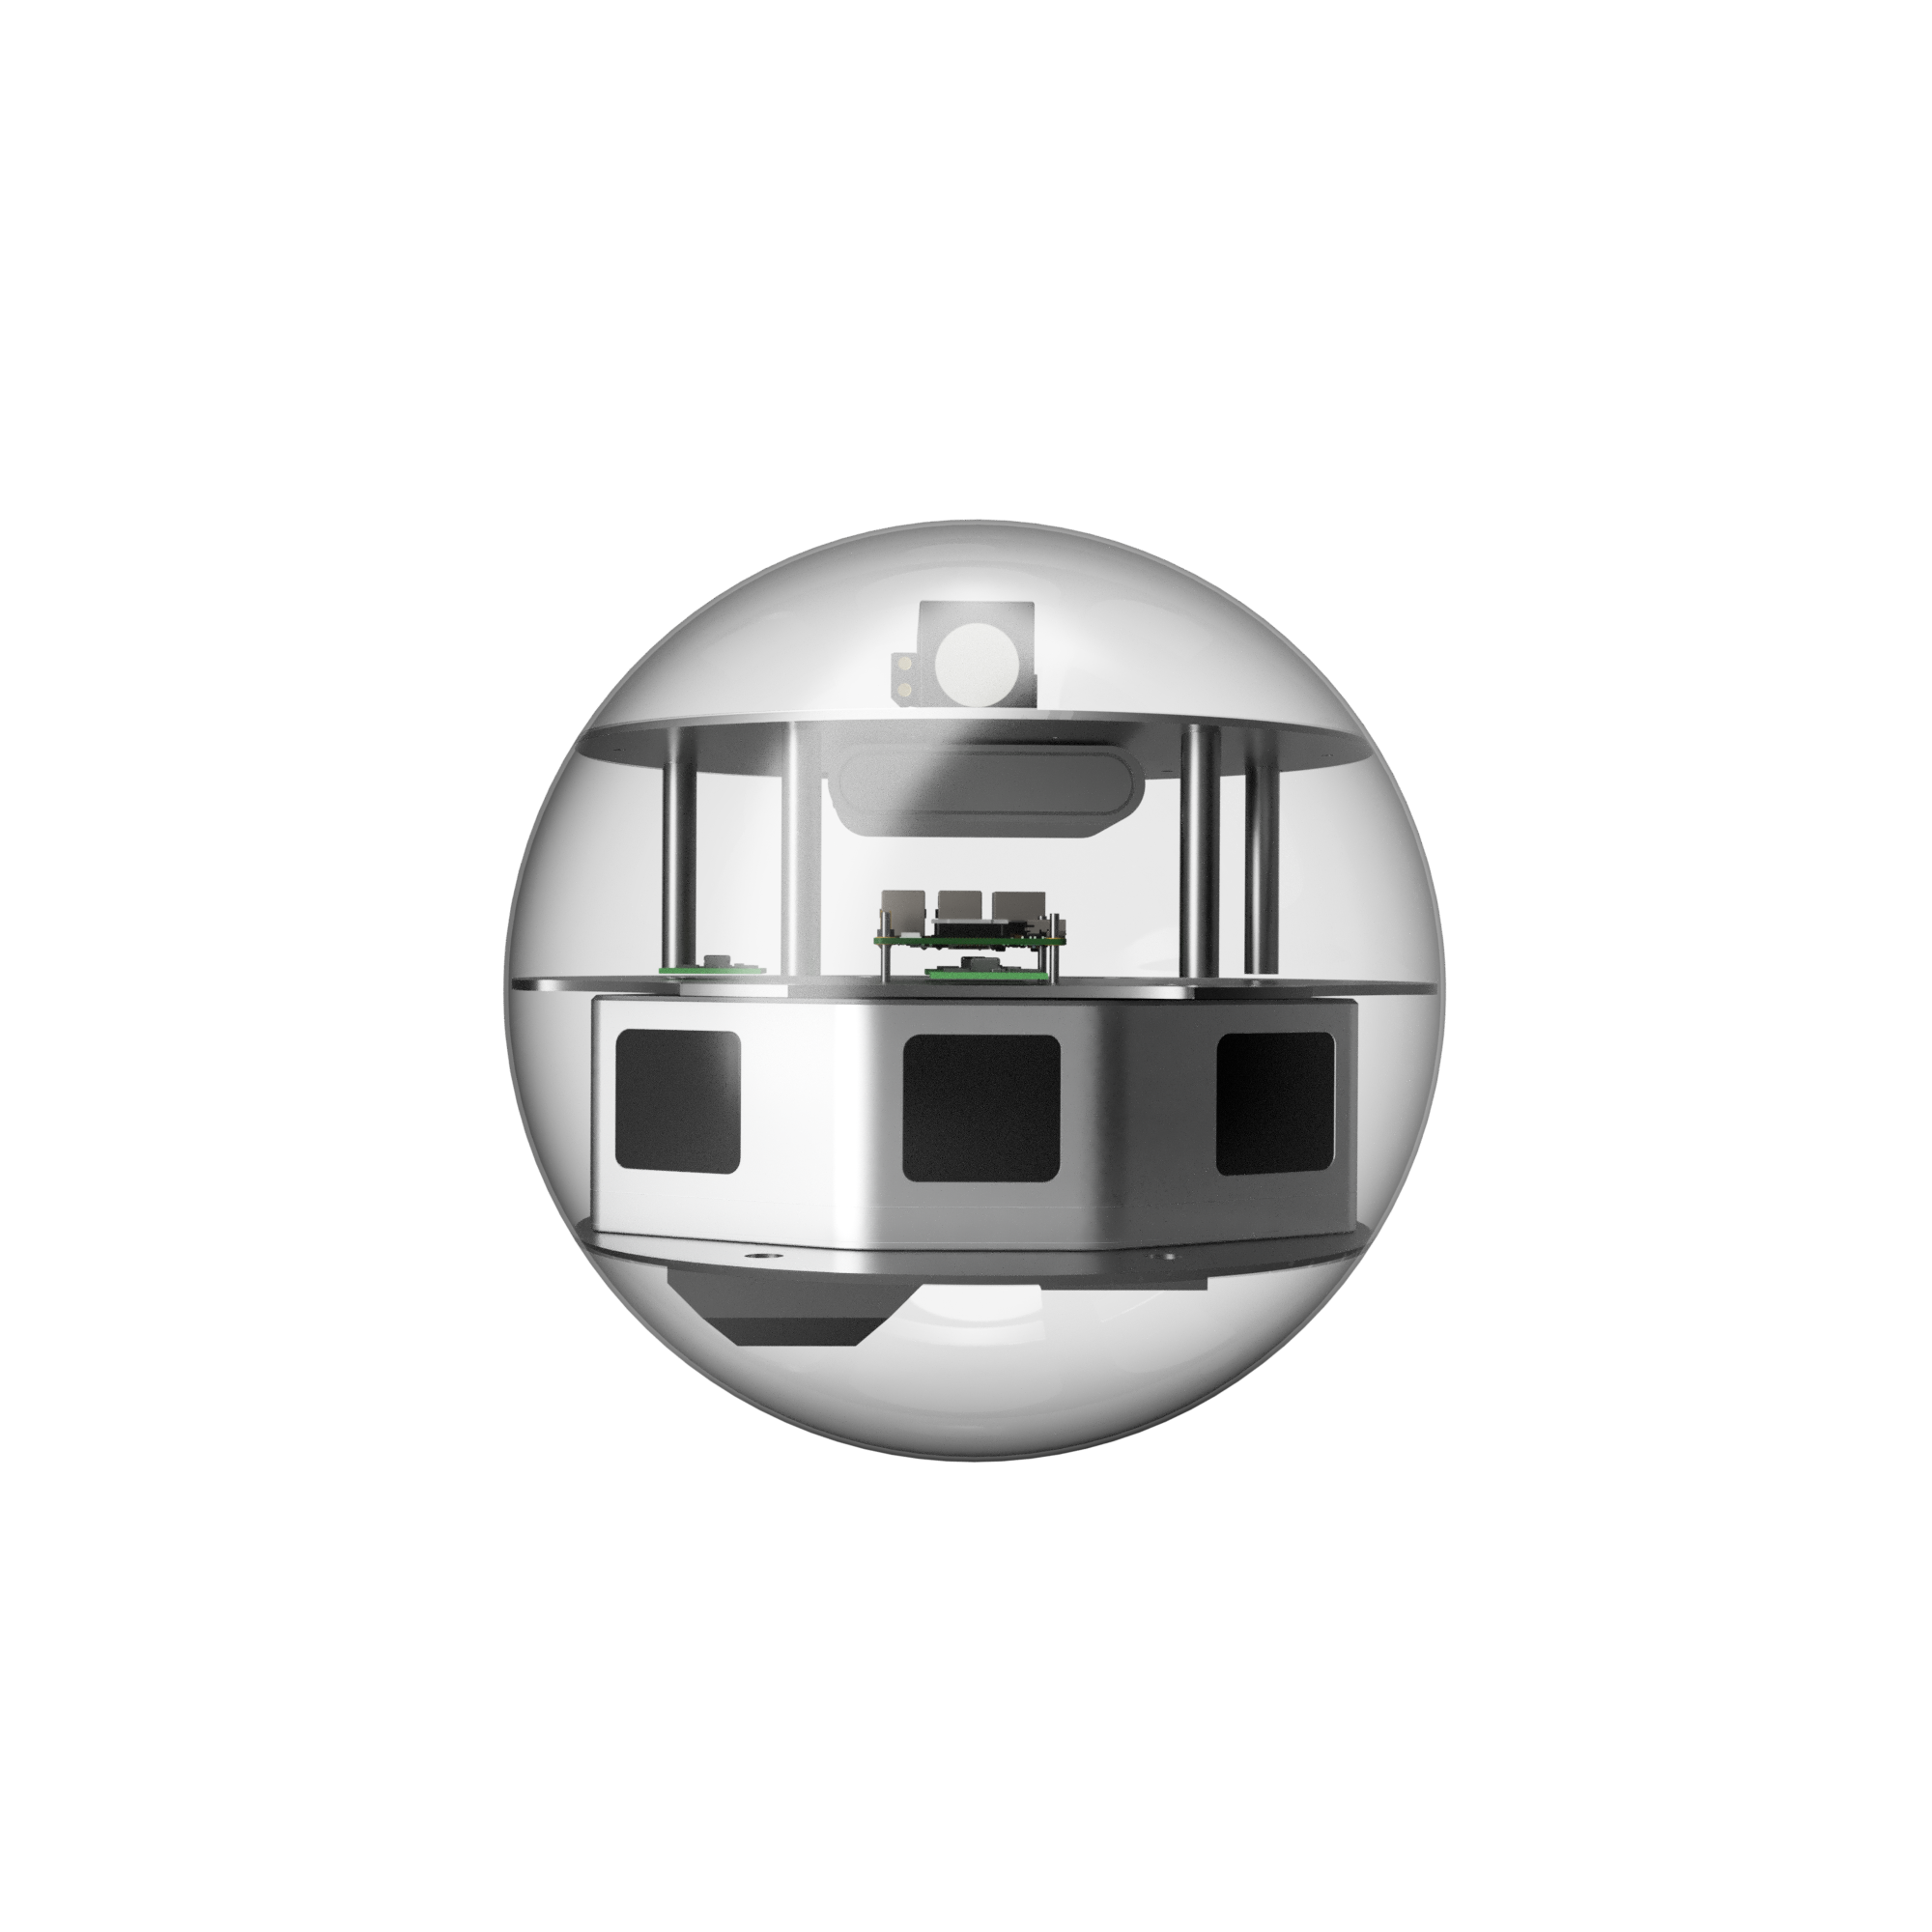
\includegraphics[width=0.495\linewidth]{./images/ProtoRoll2.png}
  \caption{\DIFaddFL{Top: Prototype used for data acquisition with the rolling sphere. The main payload is the Livox Mid-100 laser scanner. For pose-estimation, three IMUs of the manufacturer Phidget are placed inside and a Raspberry Pi 4 for the calculations. On the top are two batteries, and on the bottom one voltage stabilizer and the breakout box of the laser scanner. Below: Rendering of the simulated robot, a Livox laser scanner insider a spherical shell. }}
  \label{fig:prototype}
\end{figure}


\DIFaddend \iffalse % This is commented out because we couldn't produce results
	\subsection{RADLER}

	The second dataset is recorded using the RADLER system as described in~\cite{Borrmann2020-RADLER}.
	While not a spherical robot, this system shows many similarities with respect to its motion with a spherical robot.
	The system was manually steered along with a squared set of hallways that loop back to the initial starting point inside the old mathematics building at the University of Würzburg (denoted ``The Circle'' in~\cite{Borrmann2020-RADLER}).

	Figure~\ref{fig:radler-mathe} shows the system setup as well as the resulting point cloud.
	We see that with continuing measurement time, the drift increases, and the hallways are senses multiple times with a clear offset to each other. 

	\begin{figure*}
		\centering
		\begin{minipage}[c]{\textwidth}
			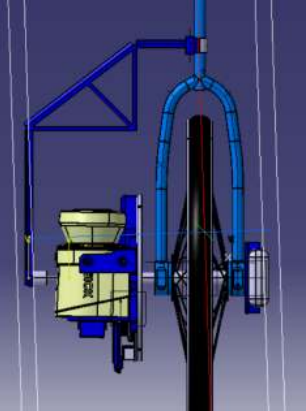
\includegraphics[width=0.2925\textwidth]{./images/radler_setup}\hfill
			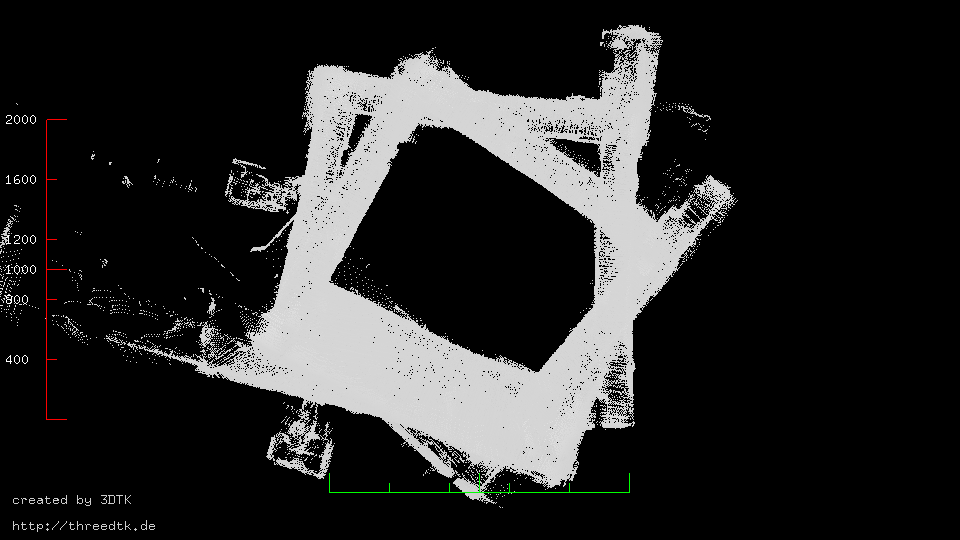
\includegraphics[width=0.7\textwidth]{./images/mathe_top_view}
		\end{minipage}
		\caption{Data acquisition using the RADLER system. Left: System setup (courtesy of Borrmann~\cite{Borrmann2020-RADLER}). Right: Unprocessed resulting point cloud.}
		\label{fig:radler-mathe}
	\end{figure*}

	\subsection{Descend Sphere REMOVE THIS SECTION}

	This was recorded using a LIVOX-Mid 100 laser scanner mounted inside a transparent shell. 
	The robot contained three Phidget 3/3/3 Spatial IMUs and was attached to a \SI{50}{\meter} tether cable that was rolled on a spool which in turn was connected to an angular encoder. 
	From these sensors, we obtained orientation information as well as height information. 
	The setup was then brought into a high indoor building (\href{https://www.sfs-w.de/feuerwehrschule/virtueller-rundgang.html}{Firefighter School in Würzburg}) where the system was manually descended from a balcony scanning the building interior.
	The robot covered a distance of approximately \SI{22}{\meter} in about \SI{402}{\second}.
	Additionally, the building was scanned using a terrestrial laser scanner to provide a reference.
	The measurements were then pre-registered before applying our plane-based correction. 
	Figure~\ref{fig:experimental-setup} shows the acquired 3D point clouds and the experimental setup. 

	\begin{figure}
		\centering
		\begin{minipage}[c]{0.25\textwidth}
			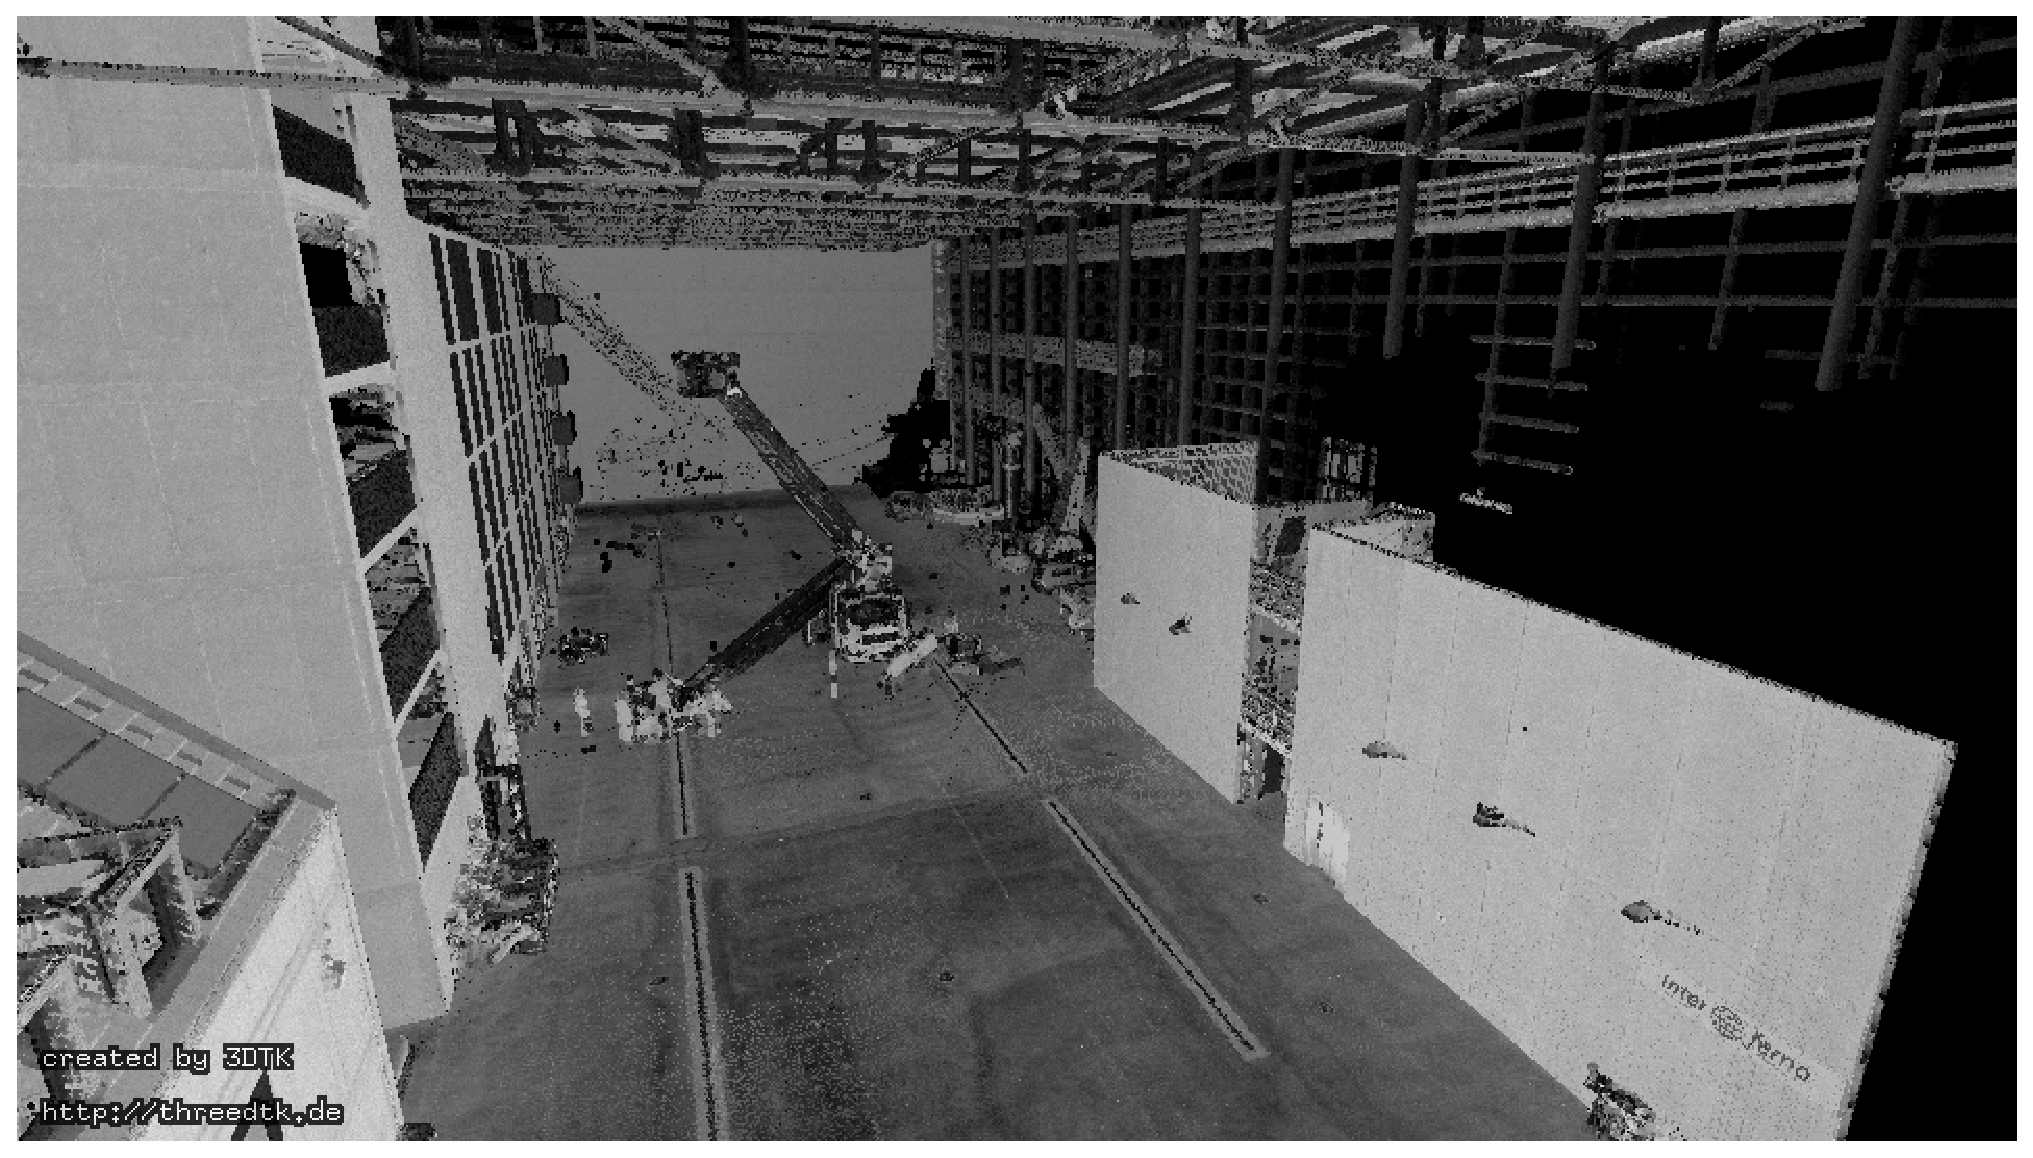
\includegraphics[width=\textwidth]{images/scan-riegl-fire}\\
			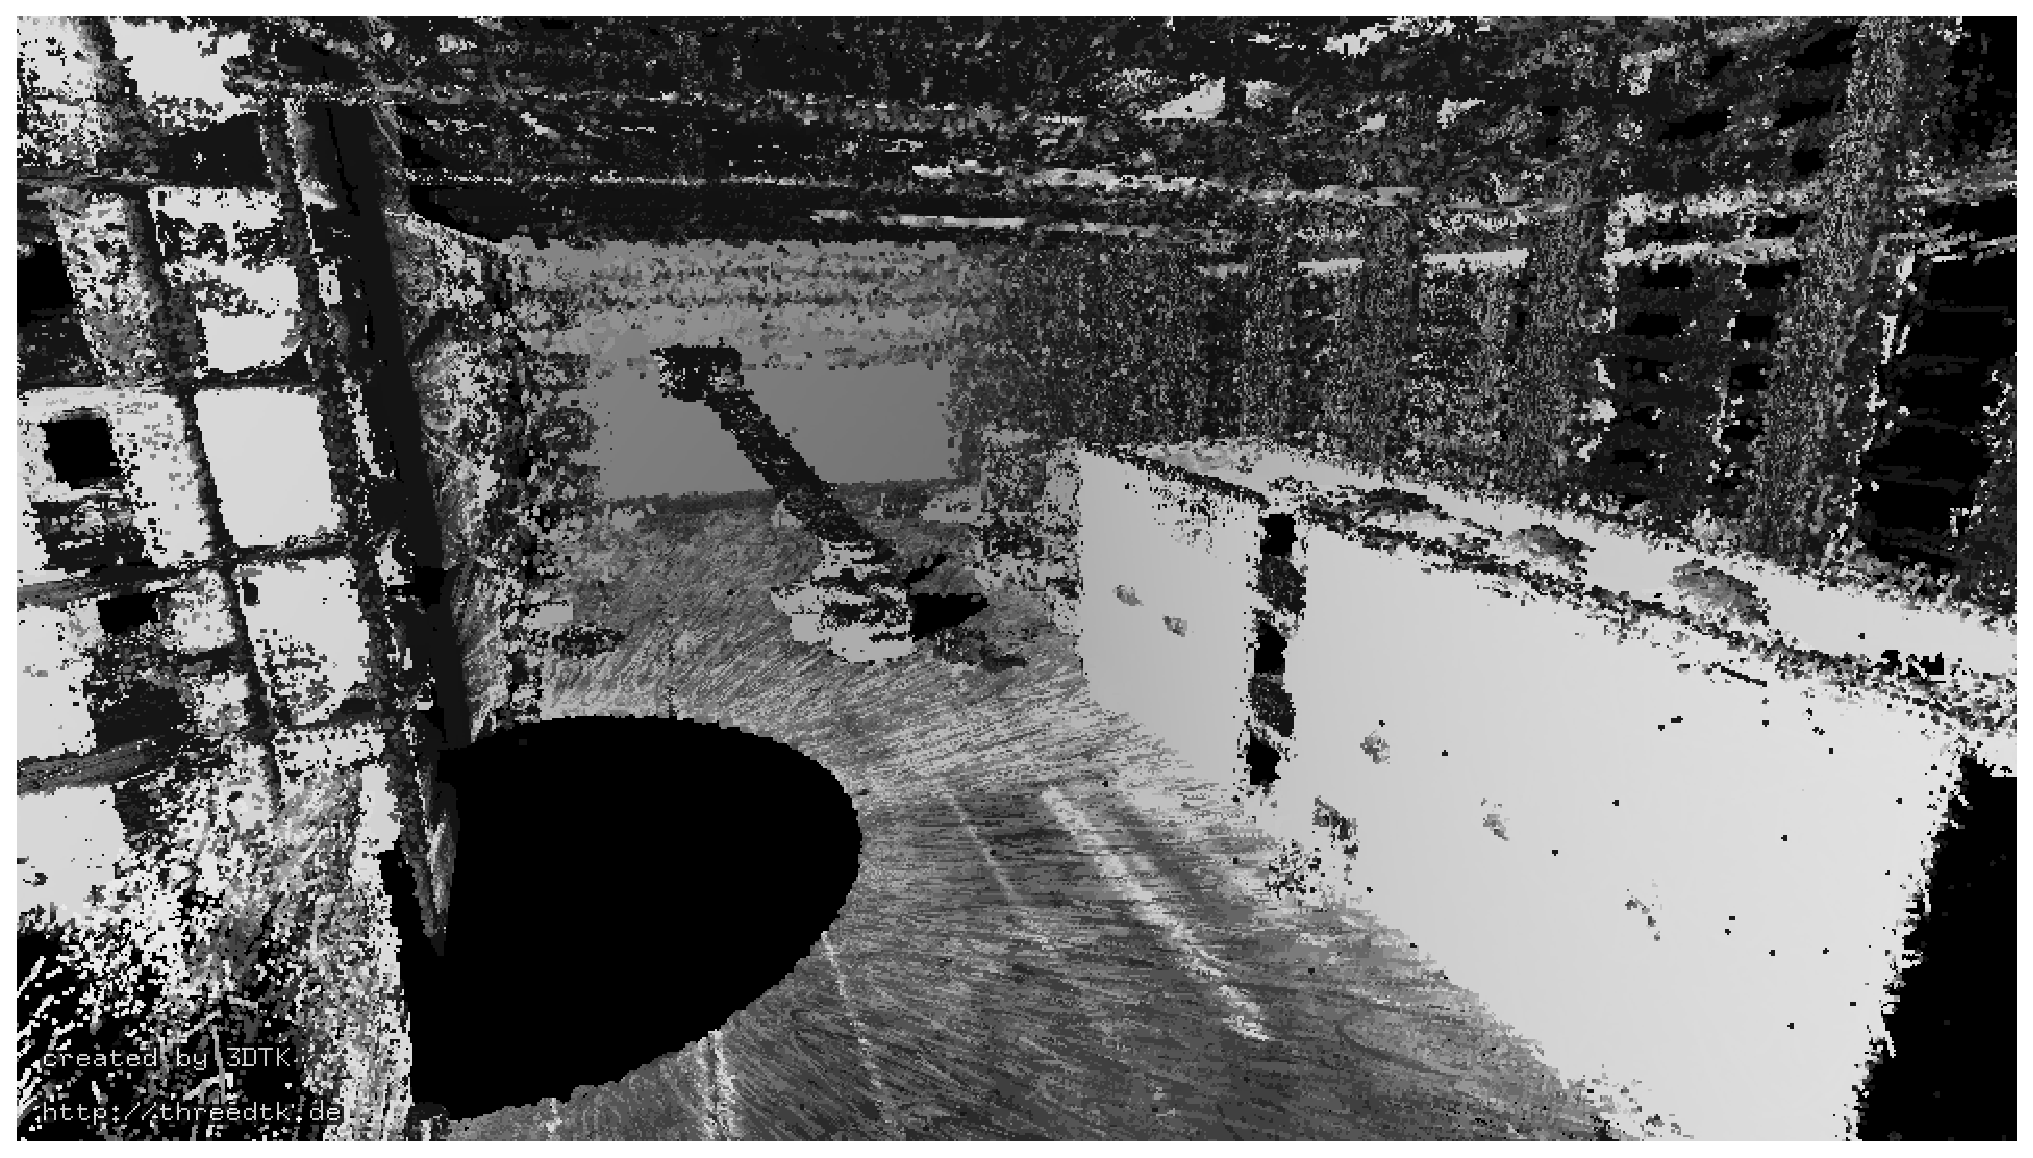
\includegraphics[width=\textwidth]{images/scan-sphere-fire}
	  	\end{minipage}\hfill
	  	\begin{minipage}[c]{0.2075\textwidth}
	  		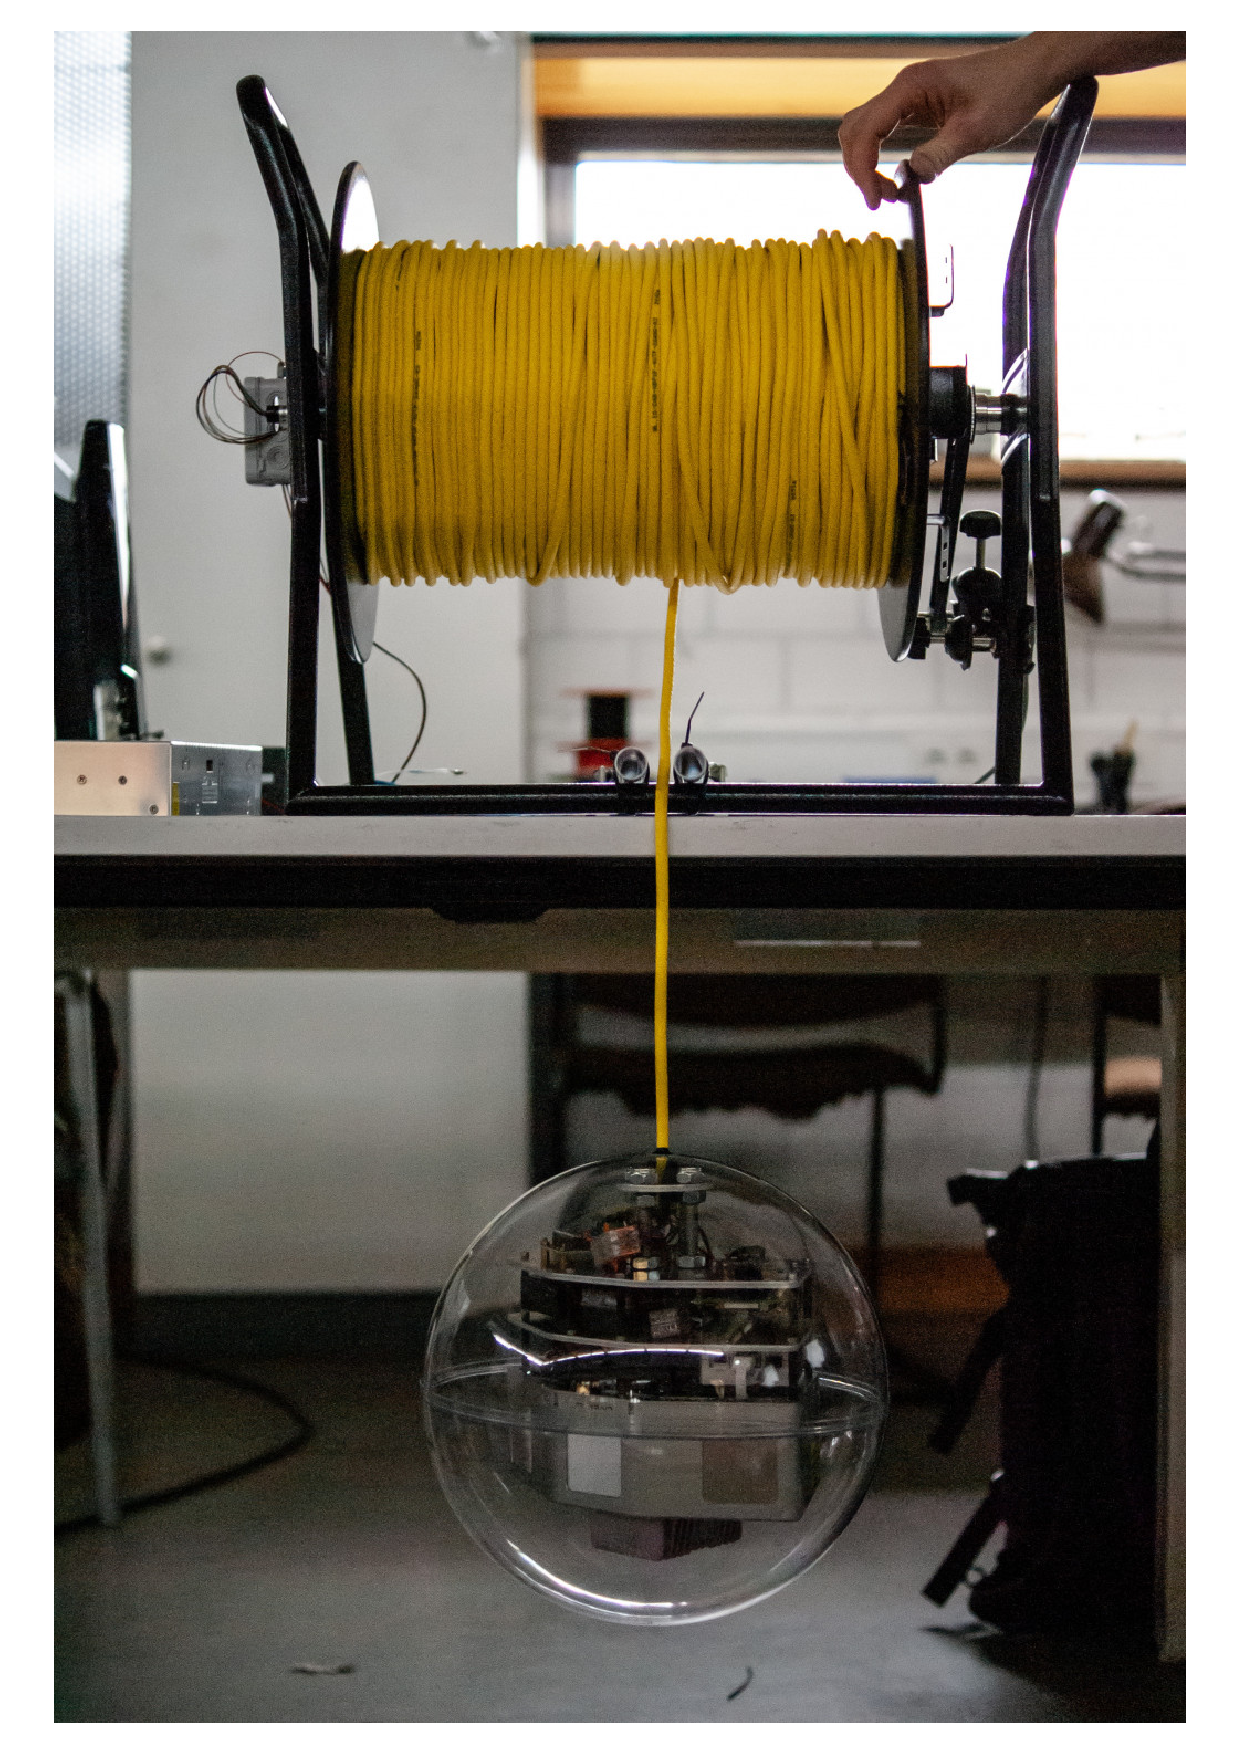
\includegraphics[width=\textwidth]{./images/lidarsetup}
	  	\end{minipage}
		\caption{Reference 3D point cloud acquired with a RIEGL 3D terrestrial laser scanner (top left). The 3D point cloud acquired by the test sphere after the pre-registration (bottom left) and a picture of the test setup (right).}
		\label{fig:experimental-setup}
	\end{figure}
\fi



%!TEX root = ../main.tex
\section{Results}

\subsection{Simulated Results}

The plane-based registration is applied to the simulated dataset with noisy pose and range measurements (cf. Figure~\ref{fig:simulatedDatasets}) without further processing.
Assuming this represents a coarsely pre-registered 3D point cloud, the distances to the ground truth were evaluated before and after the plane-based registration. 
Figure~\ref{fig:simulatedEvaluation} shows the different point-to-point distances. 

\begin{figure*}
 	\centering
 	\begin{minipage}[c]{0.495\textwidth}
 		\centering
		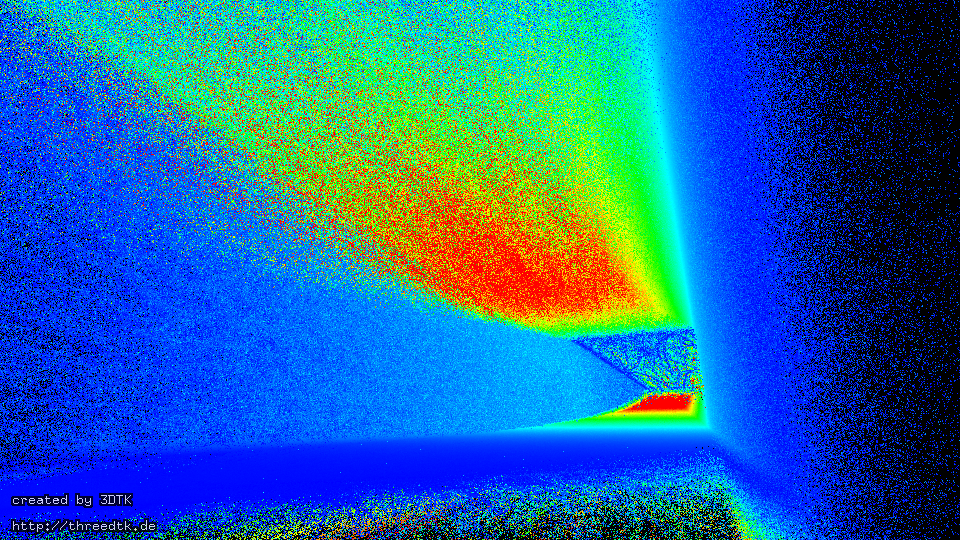
\includegraphics[width=\textwidth]{./images/uncorr_bottom_pose}\\
		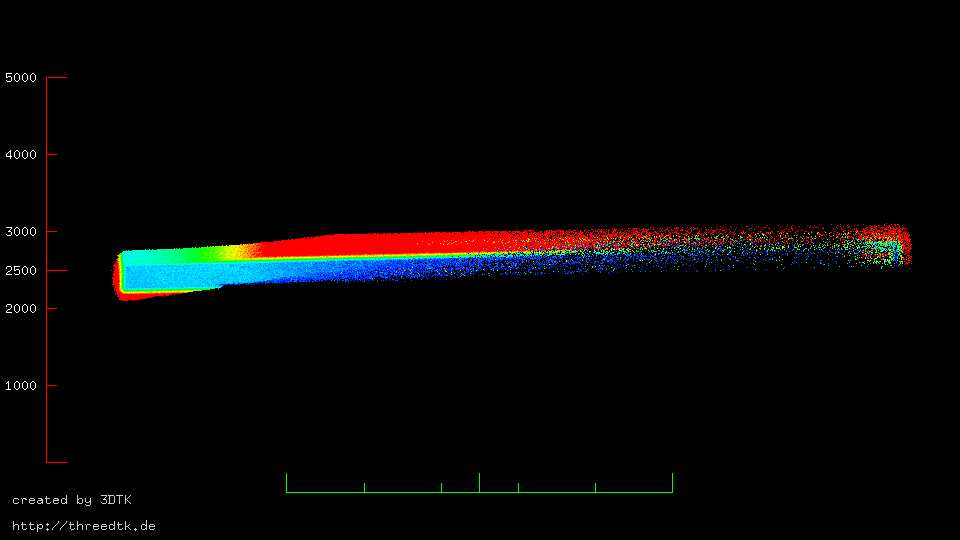
\includegraphics[width=\textwidth]{./images/uncorr_side_view}\\
  		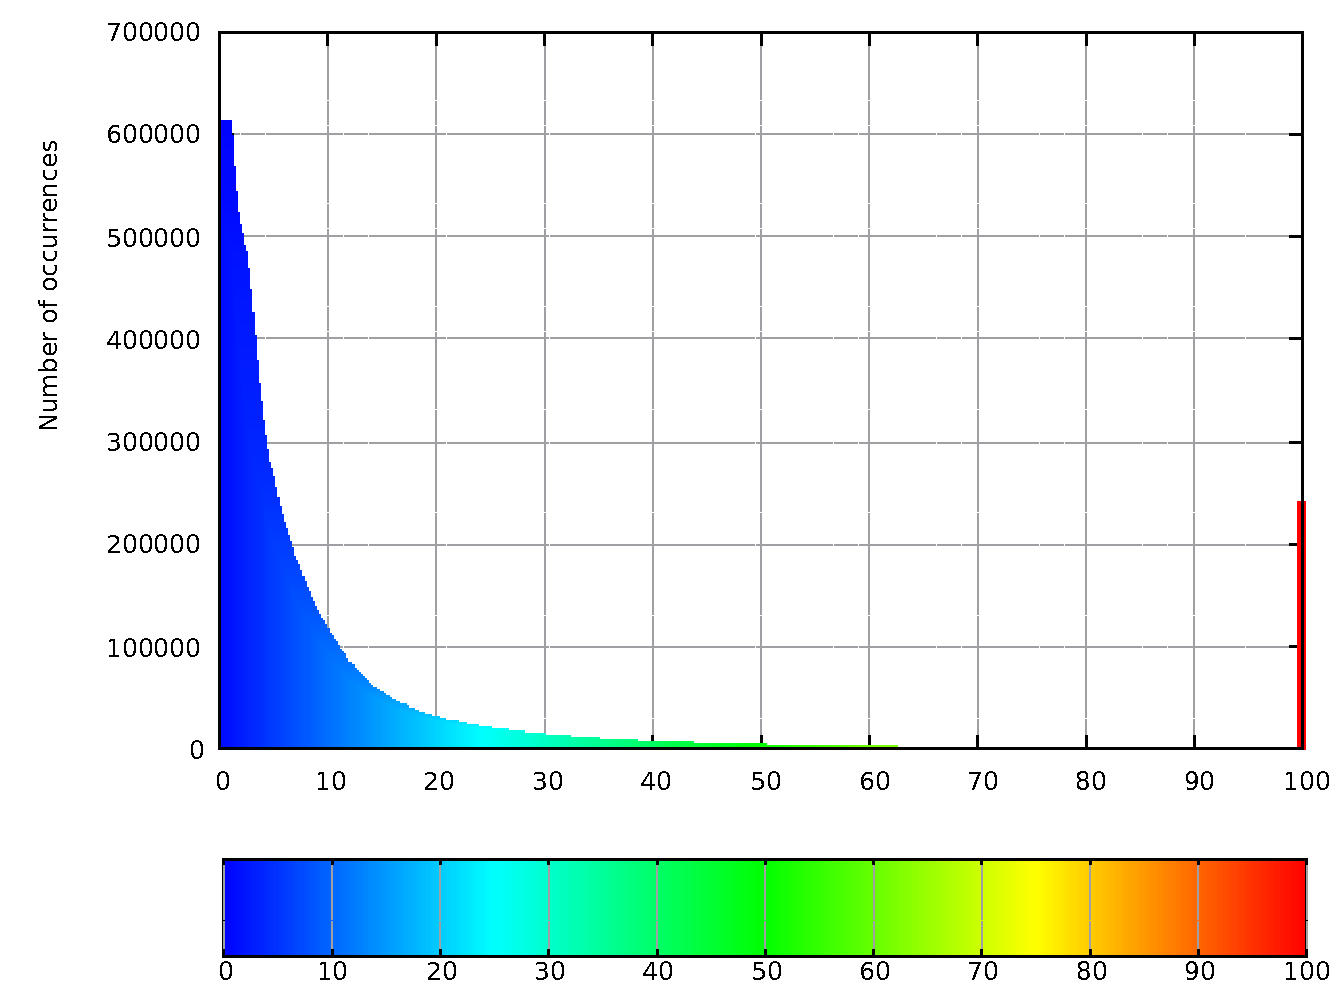
\includegraphics[width=\textwidth]{./images/uncorr_hist}
  	\end{minipage}\hfill
  	\begin{minipage}[c]{0.495\textwidth}
  		\centering
		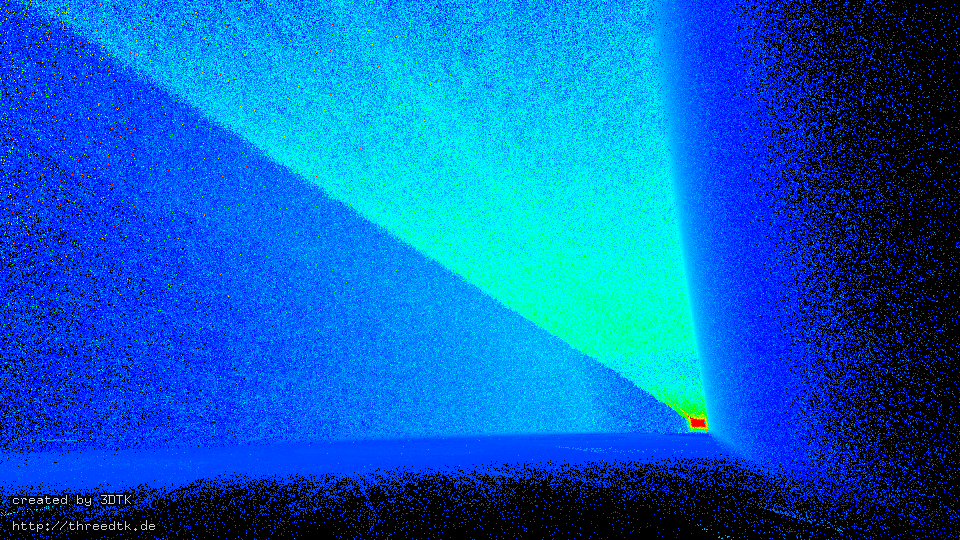
\includegraphics[width=\textwidth]{./images/corr_bottom_pose}\\
		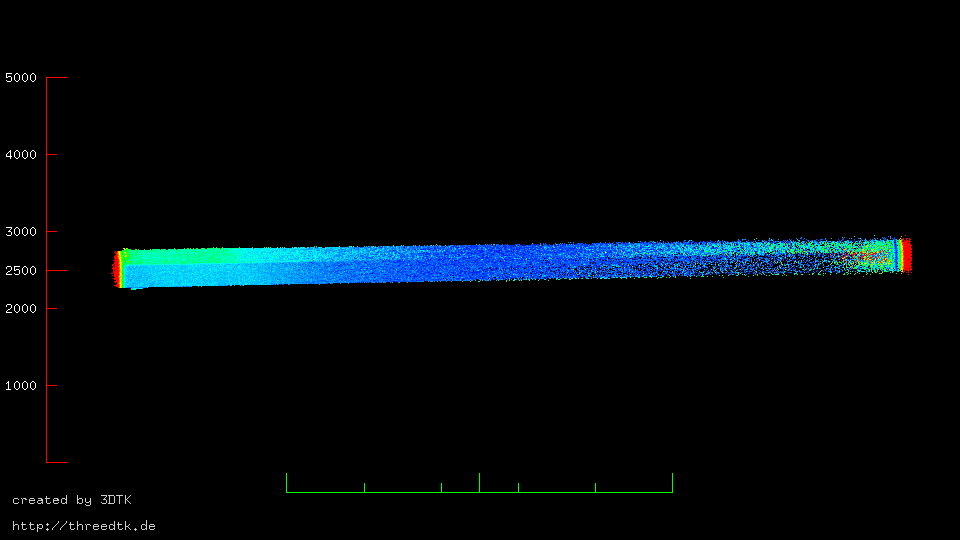
\includegraphics[width=\textwidth]{./images/corr_side_view}\\
  		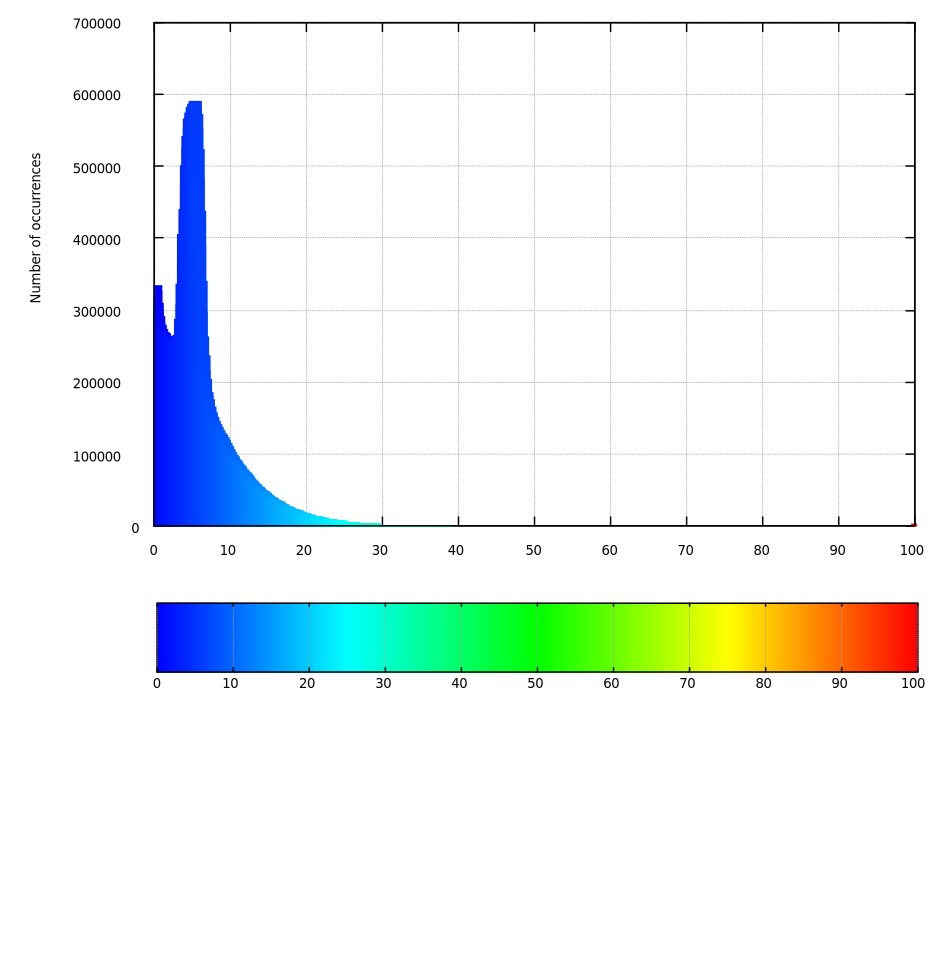
\includegraphics[width=\textwidth]{./images/corr_hist}
  	\end{minipage} 	
 	\caption{Evaluation of point distances before (left) and after (right) the plane-based registration on a simulated dataset. \DIFaddbeginFL \DIFaddFL{Lateral images always have the same orientation. }\DIFaddendFL A maximal distance of \DIFdelbeginFL \DIFdelFL{\mbox{%DIFAUXCMD
\SI{2}{m} }\hspace{0pt}%DIFAUXCMD
}\DIFdelendFL \DIFaddbeginFL \DIFaddFL{\mbox{%DIFAUXCMD
\SI{30}{m} }\hspace{0pt}%DIFAUXCMD
}\DIFaddendFL is set, such that all points that display a higher distance value are excluded from the analysis. \DIFaddbeginFL \DIFaddFL{Both point-clouds were reduced before evaluating point-to-point distances to the ground-truth. }\DIFaddendFL Further, the \DIFdelbeginFL \DIFdelFL{histogram joins }\DIFdelendFL \DIFaddbeginFL \DIFaddFL{color-space maps }\DIFaddendFL all values with a distance greater than \SI{1}{m} \DIFdelbeginFL \DIFdelFL{into }\DIFdelendFL \DIFaddbeginFL \DIFaddFL{to }\DIFaddendFL the \DIFdelbeginFL \DIFdelFL{last bucket}\DIFdelendFL \DIFaddbeginFL \DIFaddFL{same color}\DIFaddendFL . The top two columns show a heat map of distances, while the bottom shows the corresponding histogram. The color mapping is equivalent in both. An animation of the matching process is given at \DIFdelbeginFL %DIFDELCMD < \url{https://youtu.be/0ps5Pg4qo4E} %%%
\DIFdelendFL \DIFaddbeginFL \url{https://youtu.be/7igQdEeCsYk}\DIFaddendFL .} 
 	\label{fig:simulatedEvaluation}
\end{figure*} 

Before the registration, the corridor is only represented acceptably in the front part. 
The further into the corridor, i.e., the longer the robot accumulates errors, the more imprecise the data becomes. 
Finally, we see that \DIFdelbegin \DIFdel{a large portion of the data even exceeds either the \mbox{%DIFAUXCMD
\SI{1}{\meter} }\hspace{0pt}%DIFAUXCMD
error, contributing to the large spike in the histogram or even the \mbox{%DIFAUXCMD
\SI{2}{\meter} }\hspace{0pt}%DIFAUXCMD
error limit; thus , being cut from the representation}\DIFdelend \DIFaddbegin \DIFadd{many points exceed the threshold of \mbox{%DIFAUXCMD
\SI{1}{\meter} }\hspace{0pt}%DIFAUXCMD
and thus being mapped to the same color value}\DIFaddend .
After registration, we see that, qualitatively, the ideal corridor was nearly restored from the noisy data. 
In particular a very large portion of points (\DIFdelbegin \DIFdel{95}\DIFdelend \DIFaddbegin \DIFadd{90}\DIFaddend \%) have distances of less than \DIFdelbegin \DIFdel{\mbox{%DIFAUXCMD
\SI{16.6}{\centi\meter}}\hspace{0pt}%DIFAUXCMD
}\DIFdelend \DIFaddbegin \DIFadd{\mbox{%DIFAUXCMD
\SI{35.9}{\centi\meter}}\hspace{0pt}%DIFAUXCMD
}\DIFaddend .
Table~\ref{tab:percentiles} shows the comparison of further percentiles of both datasets. 

\begin{table}
	\centering
	\begin{tabular}{@{}lccc@{}}\hline
		& P90 & P95 & P98 \\ \hline\hline
		Uncorrected & \DIFdelbeginFL \DIFdelFL{\mbox{%DIFAUXCMD
\SI{24.2}{\centi\meter} }\hspace{0pt}%DIFAUXCMD
}\DIFdelendFL \DIFaddbeginFL \DIFaddFL{\mbox{%DIFAUXCMD
\SI{372.1}{\centi\meter} }\hspace{0pt}%DIFAUXCMD
}\DIFaddendFL &  \DIFdelbeginFL \DIFdelFL{\mbox{%DIFAUXCMD
\SI{38.2}{\centi\meter} }\hspace{0pt}%DIFAUXCMD
}\DIFdelendFL \DIFaddbeginFL \DIFaddFL{\mbox{%DIFAUXCMD
\SI{553.4}{\centi\meter} }\hspace{0pt}%DIFAUXCMD
}\DIFaddendFL &  \DIFdelbeginFL \DIFdelFL{\mbox{%DIFAUXCMD
\SI{61.5}{\centi\meter} }\hspace{0pt}%DIFAUXCMD
}\DIFdelendFL \DIFaddbeginFL \DIFaddFL{\mbox{%DIFAUXCMD
\SI{827.9}{\centi\meter} }\hspace{0pt}%DIFAUXCMD
}\DIFaddendFL \\%& \SI{9.7}{\centi\meter}\\
		Corrected & \DIFdelbeginFL \DIFdelFL{\mbox{%DIFAUXCMD
\SI{12.8}{\centi\meter} }\hspace{0pt}%DIFAUXCMD
}\DIFdelendFL \DIFaddbeginFL \DIFaddFL{\mbox{%DIFAUXCMD
\SI{35.9}{\centi\meter} }\hspace{0pt}%DIFAUXCMD
}\DIFaddendFL &  \DIFdelbeginFL \DIFdelFL{\mbox{%DIFAUXCMD
\SI{16.6}{\centi\meter} }\hspace{0pt}%DIFAUXCMD
}\DIFdelendFL \DIFaddbeginFL \DIFaddFL{\mbox{%DIFAUXCMD
\SI{64.1}{\centi\meter} }\hspace{0pt}%DIFAUXCMD
}\DIFaddendFL &  \DIFdelbeginFL \DIFdelFL{\mbox{%DIFAUXCMD
\SI{21.6}{\centi\meter} }\hspace{0pt}%DIFAUXCMD
}\DIFdelendFL \DIFaddbeginFL \DIFaddFL{\mbox{%DIFAUXCMD
\SI{122.8}{\centi\meter} }\hspace{0pt}%DIFAUXCMD
}\DIFaddendFL \\\hline%& \SI{6.3}{\centi\meter}\\ \hline
	\end{tabular}
	\caption{Comparison of point-distances in the uncorrected and corrected simulated dataset.}
	\label{tab:percentiles}
\end{table}

Further, the square and straight shape of the corridor is restored well, and especially the large \DIFdelbegin \DIFdel{spike at }\DIFdelend \DIFaddbegin \DIFadd{amount of points with an }\DIFaddend errors of greater than \SI{1}{m} is removed. 
Any such errors tend to occur at the back and the front of the corridor where the measured range is the largest hence has the largest contribution of the range error. 

\subsection{Floating Sphere Results}

Figure~\ref{fig:cylon-corrected} shows the results obtained before and after employing the plane based registration on the dataset acquired by the floating sphere.
The pre-registration is obtained by determining the orientation of the sphere via Madgwick filtered~\cite{madgwick2010efficient} IMU measurements.
\DIFdelbegin \DIFdel{We combine ten }\DIFdelend \DIFaddbegin \DIFadd{To increase the number of possible point-to-plane correspondences we combine twenty temporally successive }\DIFaddend scans into one meta-scan, which is then globally registered. 
\DIFaddbegin \DIFadd{We always use the scan at the median index as a reference coordinate system.
}\DIFaddend This does not only speed up convergence due to the proportional effect on the error function but also decreases the risk of transforming \DIFdelbegin \DIFdel{the scan in a senseless way}\DIFdelend \DIFaddbegin \DIFadd{a single line scan incorrectly}\DIFaddend .
Transformations like these happen \DIFdelbegin \DIFdel{when incorrectly labeled points have a huge effect on the error gradient, which is especially the case when considering only a few points }\DIFdelend \DIFaddbegin \DIFadd{in particular for a small collection of points as outliers have more influence}\DIFaddend .

\begin{figure*}
	\centering
	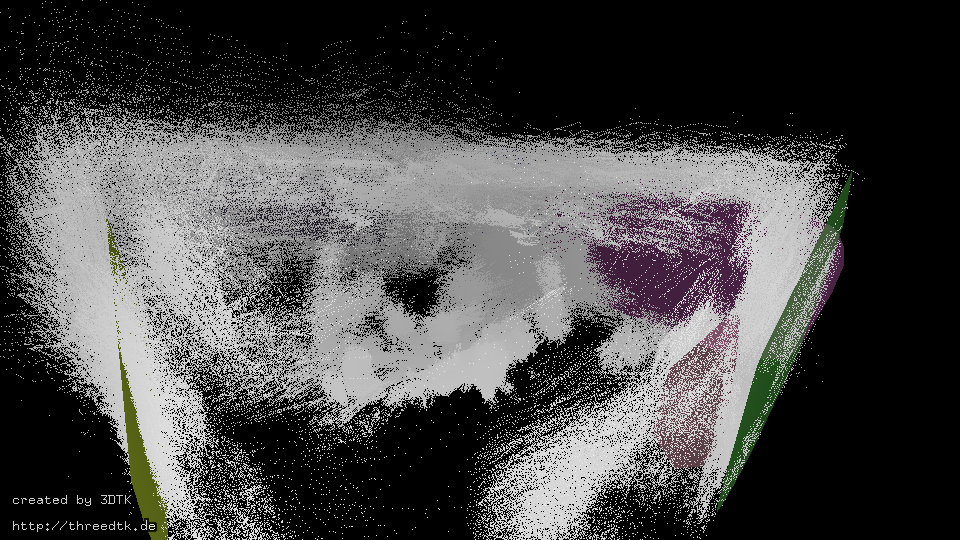
\includegraphics[width=0.495\textwidth]{./images/cylon_uncorr_corner}\hfill
	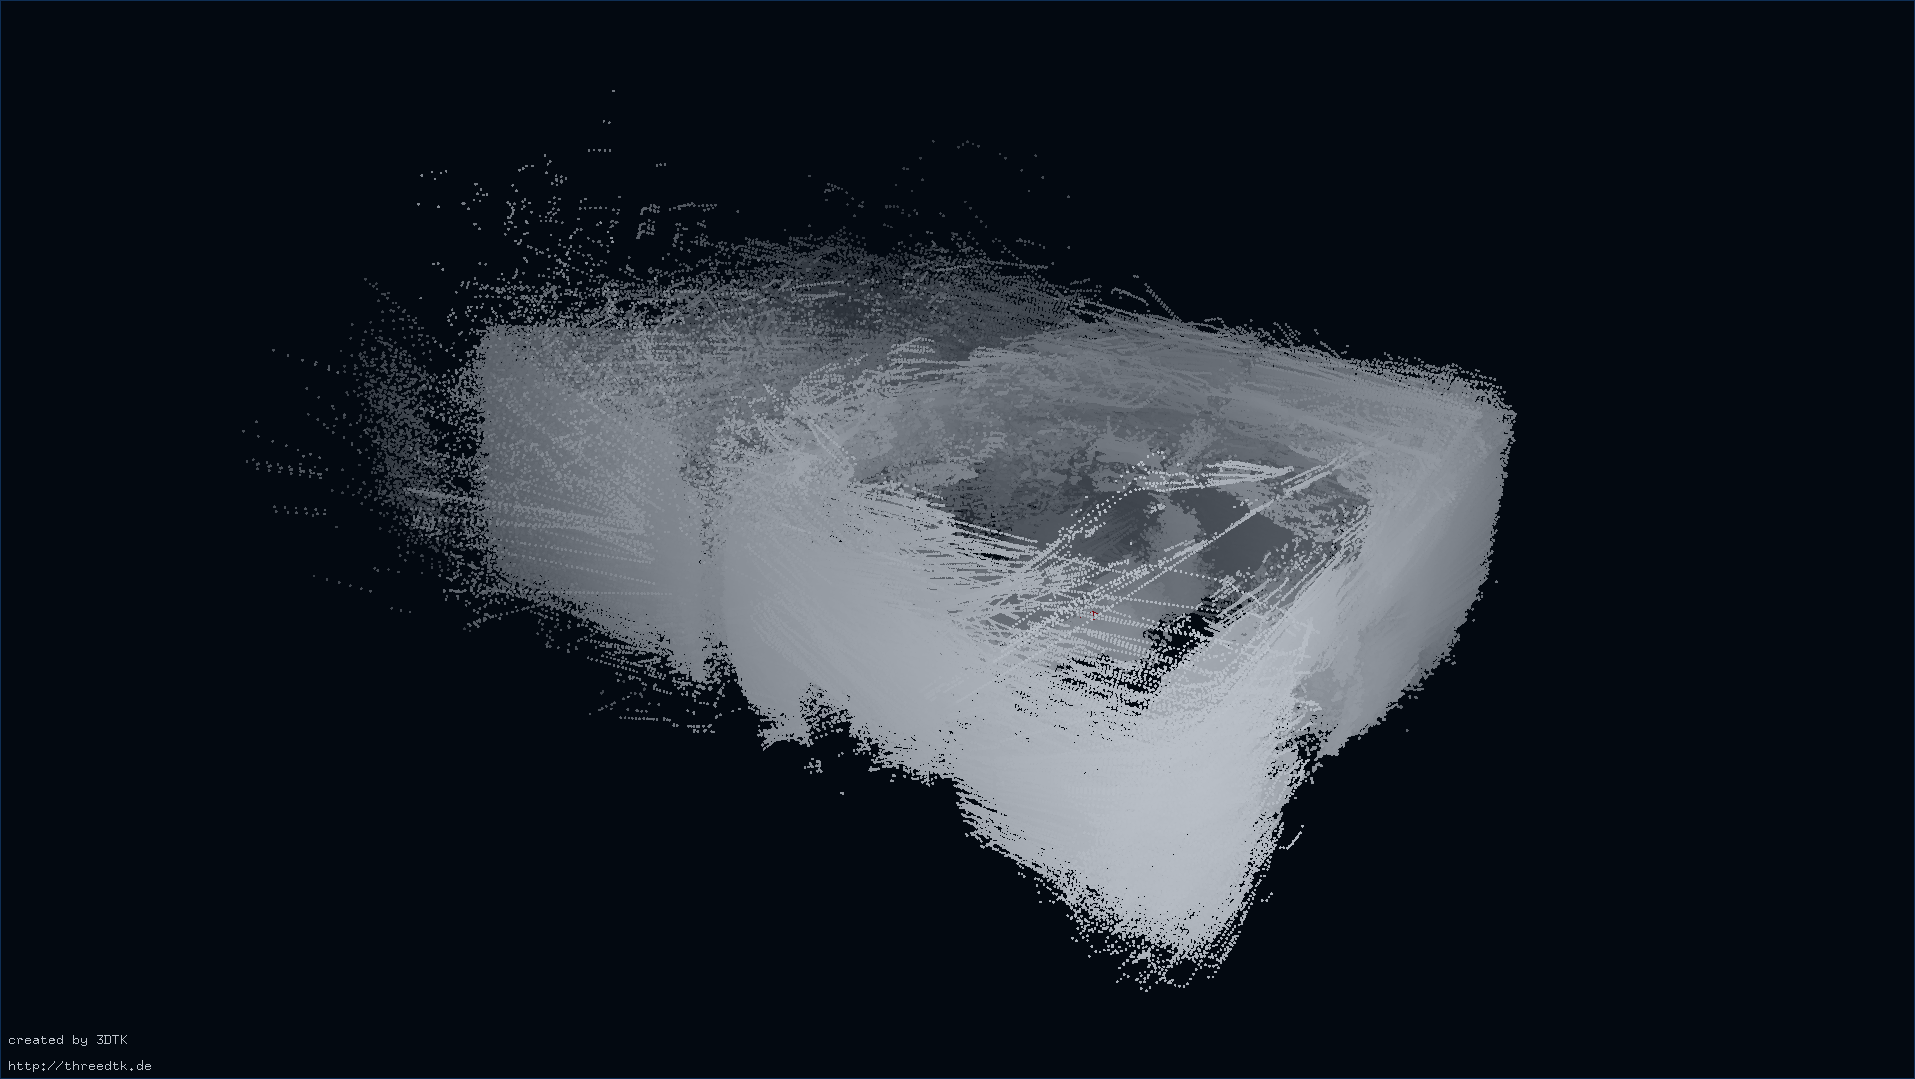
\includegraphics[width=0.495\textwidth]{./images/cylon_corr_corner}\\
	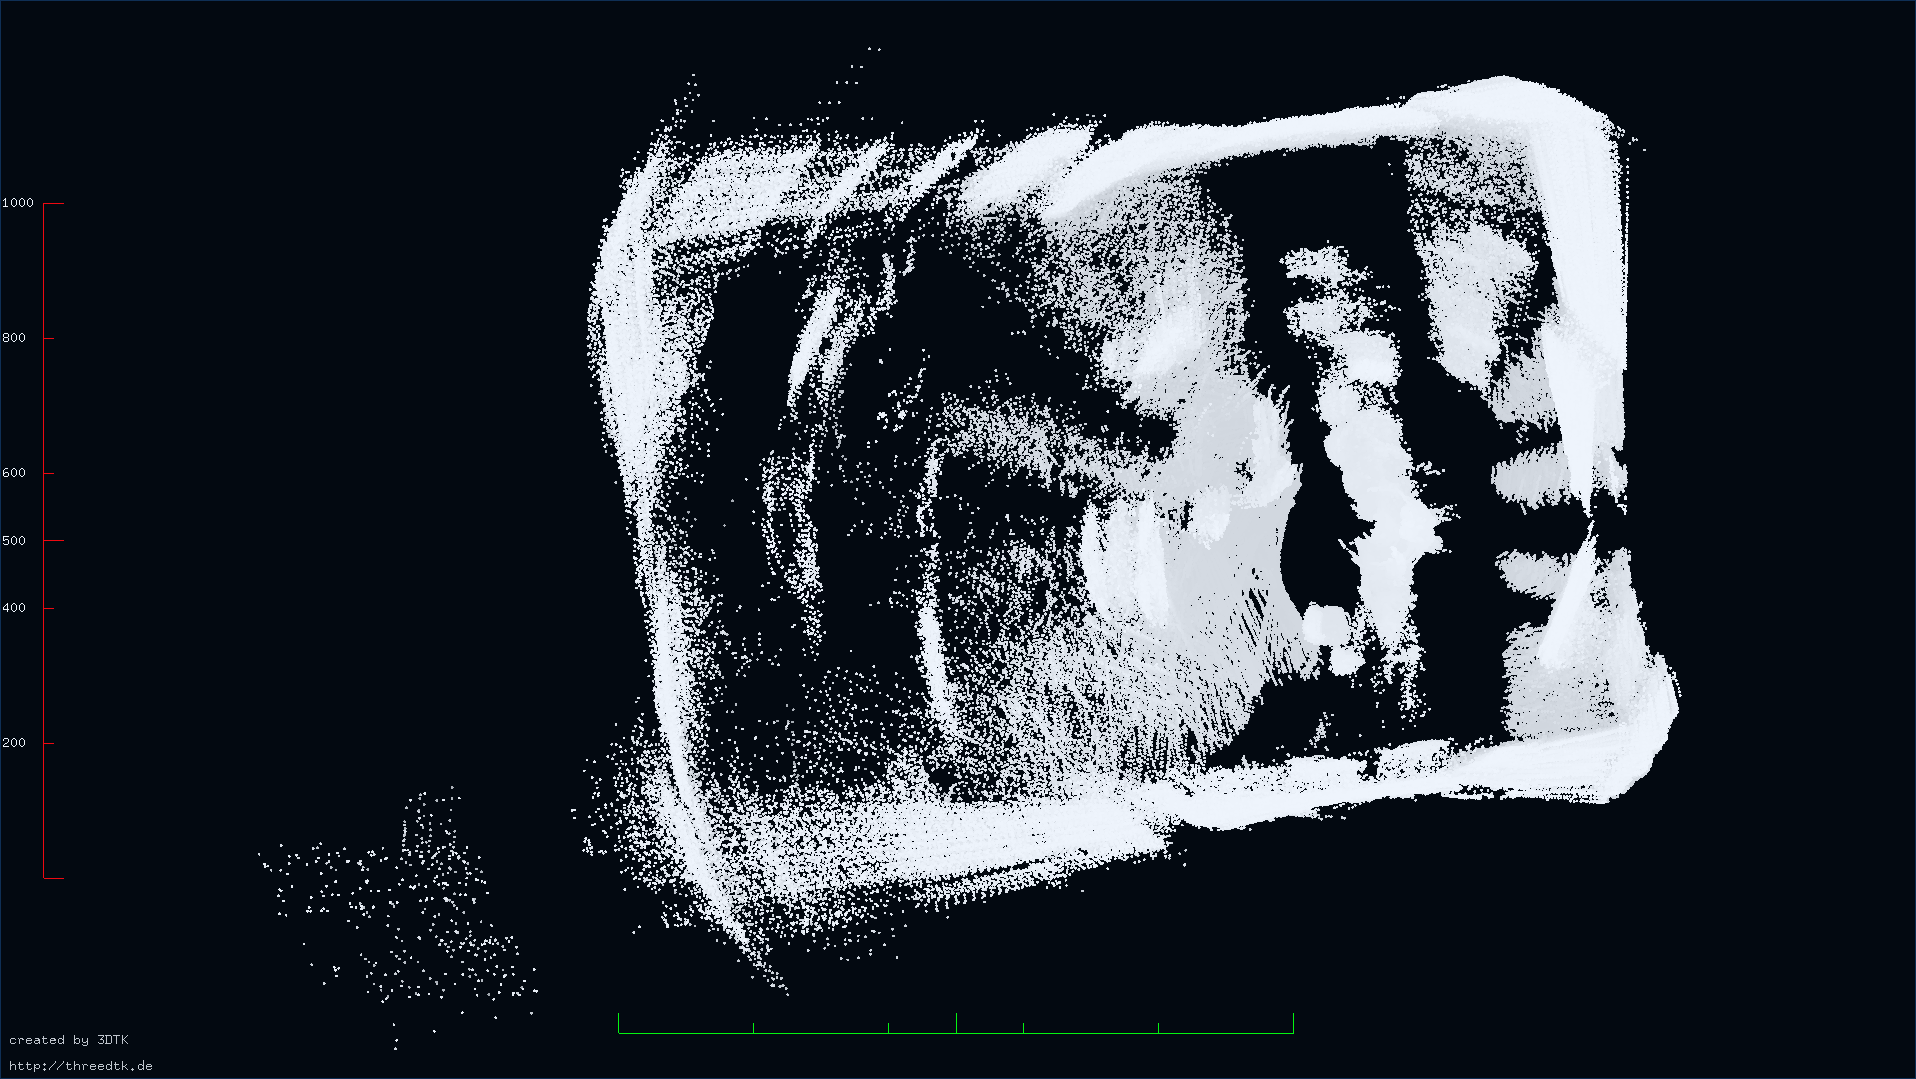
\includegraphics[width=0.495\textwidth]{./images/cylon_uncorr_top}\hfill
	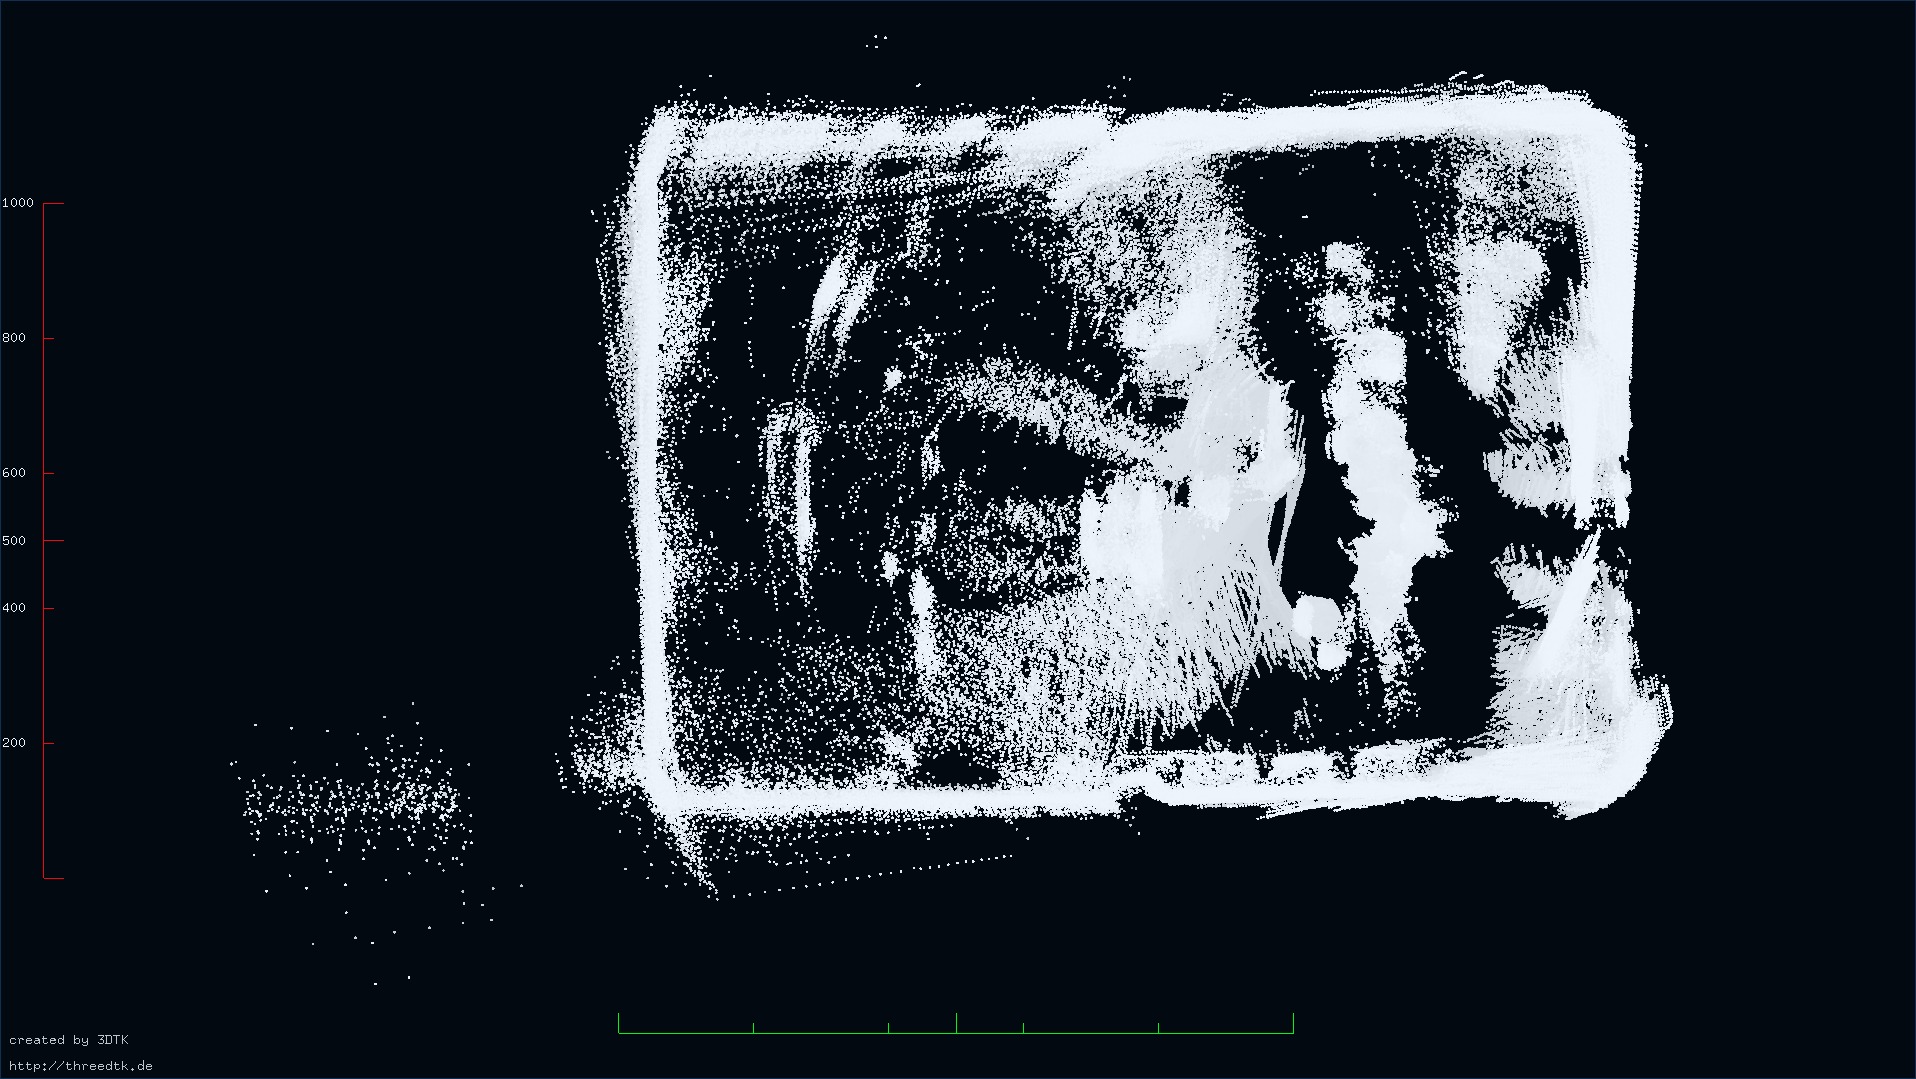
\includegraphics[width=0.495\textwidth]{./images/cylon_corr_top}
	\caption{The point cloud acquired by the floating sphere before (left) and after (right) applying the plane based registration. View from the interior \DIFdelbeginFL \DIFdelFL{that shows the used planes }\DIFdelendFL (top) and a birds-eye view (bottom). \DIFaddbeginFL \DIFaddFL{Parameters used for optimization: $\epsilon_H = 50$, $\epsilon_P = 200$, $\epsilon_\alpha = \frac{\pi}{4}$, $K = 20$ for AKNN, $d_{growth} = 50$, $N_{c_min} = 200$, $\alpha_0 = [0.01, 0.01, 0.01, 0, 0, 0]^\tau$, $i = 8$, $k = 100$. }\DIFaddendFL An animation of the registration process is given at \DIFdelbeginFL %DIFDELCMD < \url{https://youtu.be/8XdIUN_9VpY} %%%
\DIFdelendFL \DIFaddbeginFL \url{https://youtu.be/Qa2Qi8z0KEk} \DIFaddendFL .}
	\label{fig:cylon-corrected}
\end{figure*}
After the registration, the walls of the room are significantly more prominent in the point cloud. 
In particular, the noise in the top left corner of the top view (cf. figure~\ref{fig:cylon-corrected}) has been visibly reduced.
Further, the deviation of points around the walls is notably smaller as the points are moved on the plane.

\DIFdelbegin \DIFdel{However, some imprecisions remain.
In particular, at the initially very noisy top left corner of the top view, a few points cannot be matched to the plane. 
The scans that cause these imprecisions are problematic as they measure a number of plane-like structures in the interior of the room.
When relabeling those scans, the interior points are associated with a plane , and hence the corresponding distance is minimized}\DIFdelend \DIFaddbegin \subsection{\DIFadd{Rolling Sphere Results}}

\DIFadd{Figure~\ref{fig:jasperhome} shows the results obtained before and after employing the presented algorithm on the dataset, acquired by the prototype in figure~\ref{fig:prototype}.
We again combine twenty temporally successive scans into one meta-scan, using the scan at the median index as a reference coordinate system, which is then globally registered.
We used the first seven of these meta-scans, corresponding to the first full rotation of the spher, to extract global planes.
All subsequent meta-scans are then matched against the initial global plane model.
We use both optimizations from section \ref{ssec:furtheropts}, introducing a global up/down lock for gradient descent and applying sequential iteration to eliminate accumulating pose error.
}


\begin{figure*}
        \centering
        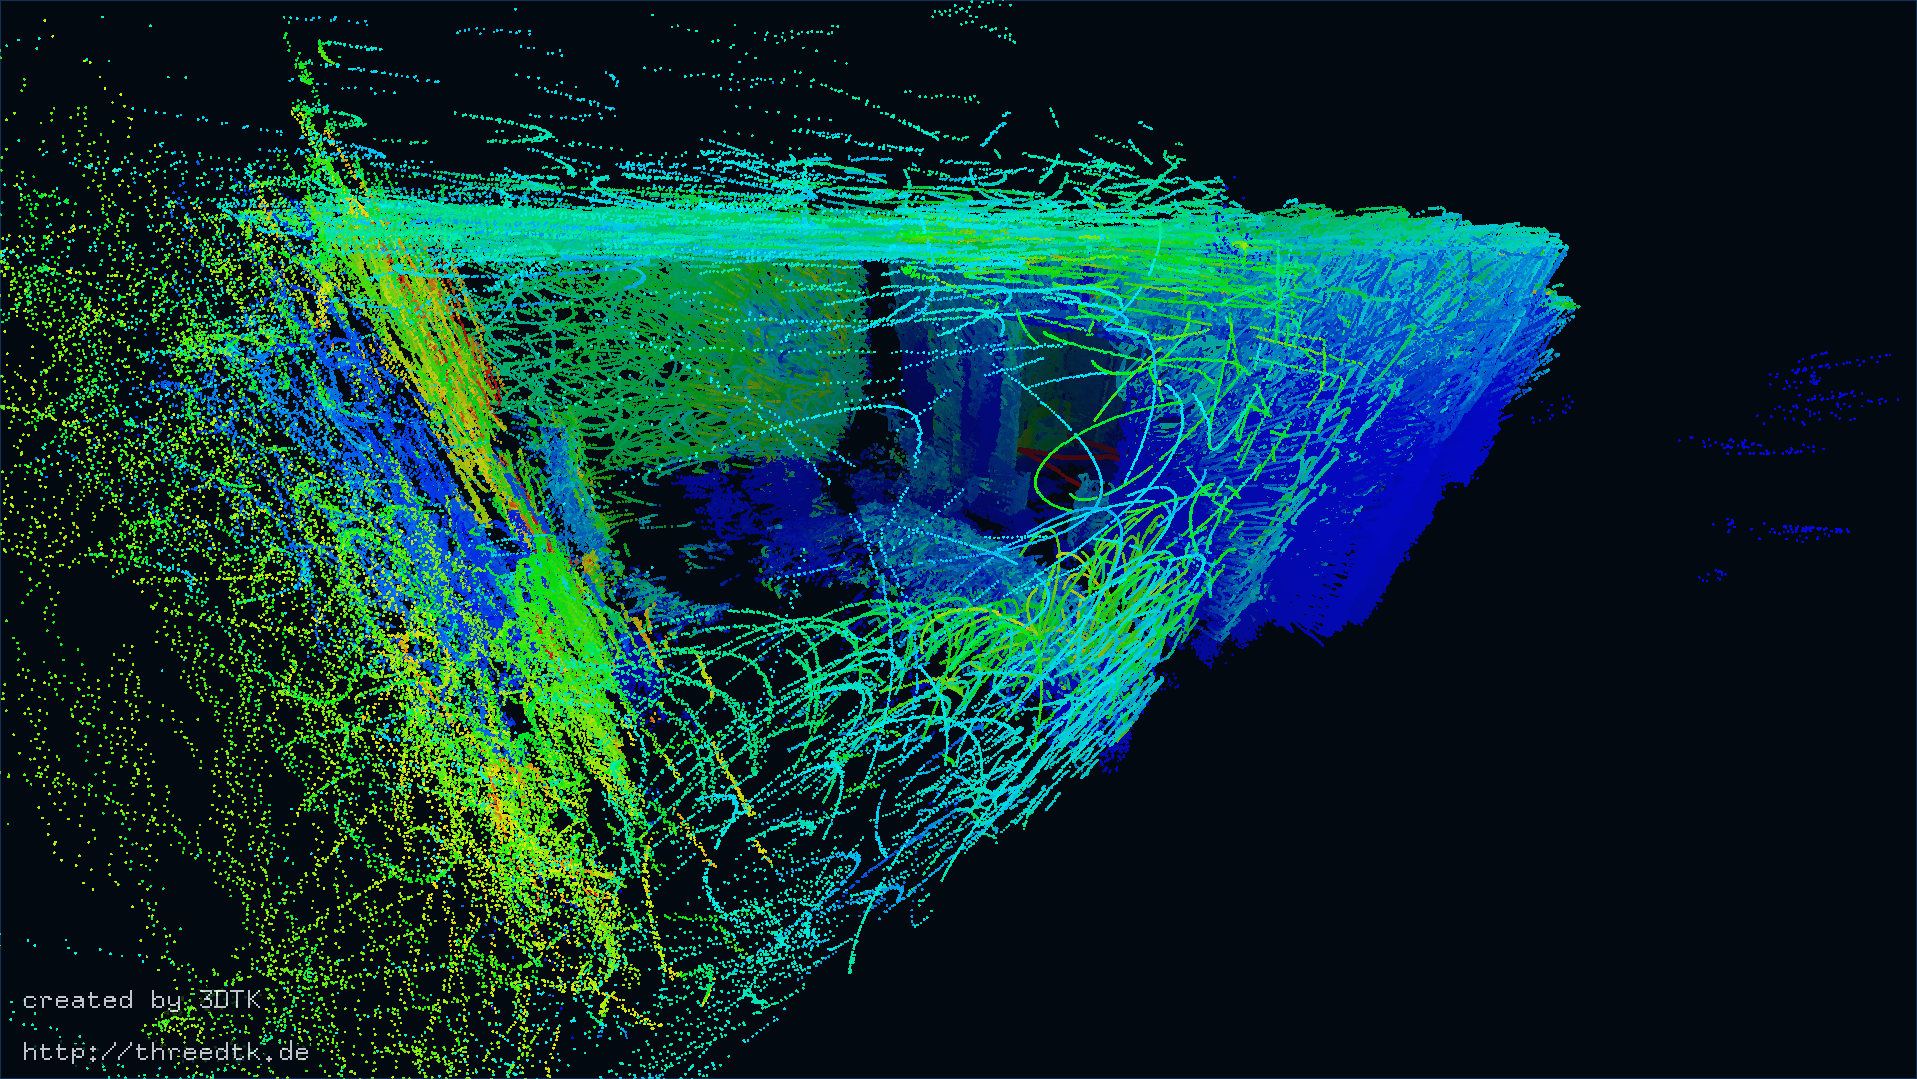
\includegraphics[width=0.495\textwidth]{./images/jasper_uncorr_corner}\hfill
        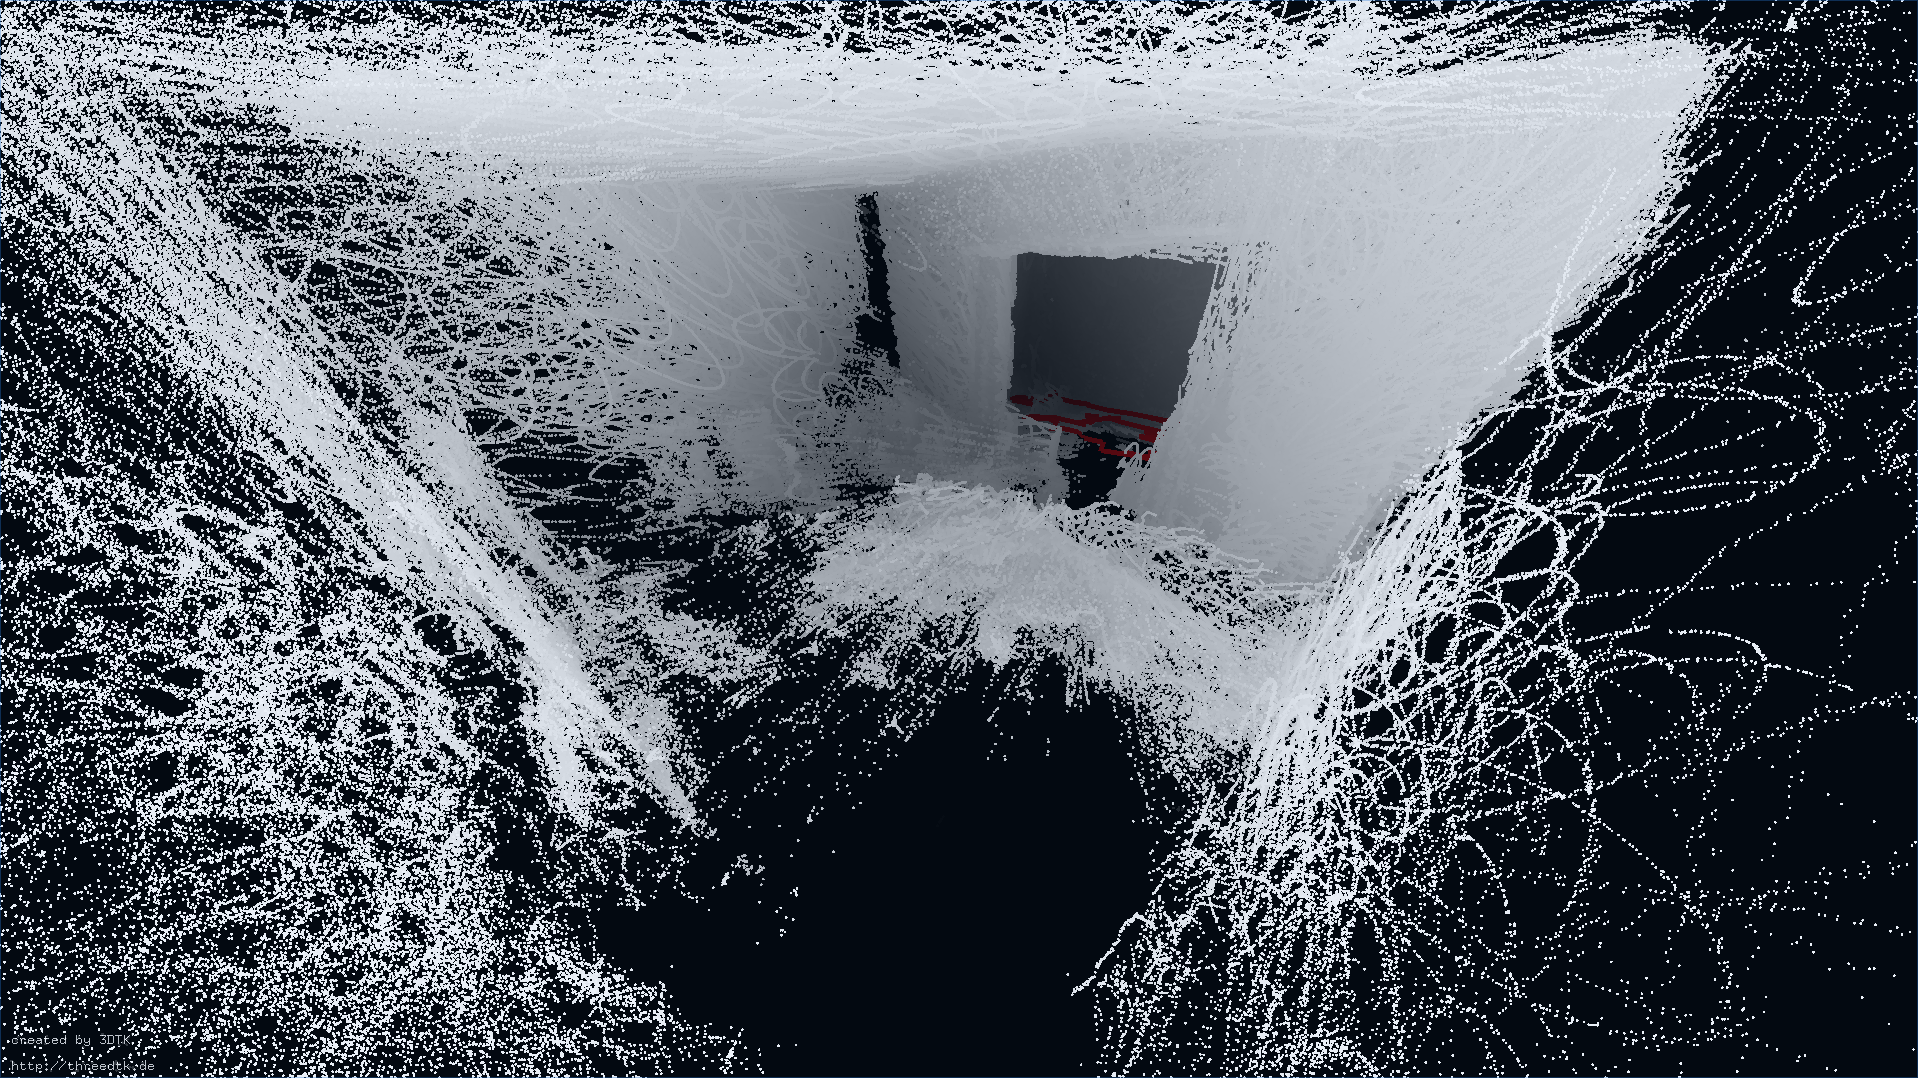
\includegraphics[width=0.495\textwidth]{./images/jasper_corr_corner}\\
	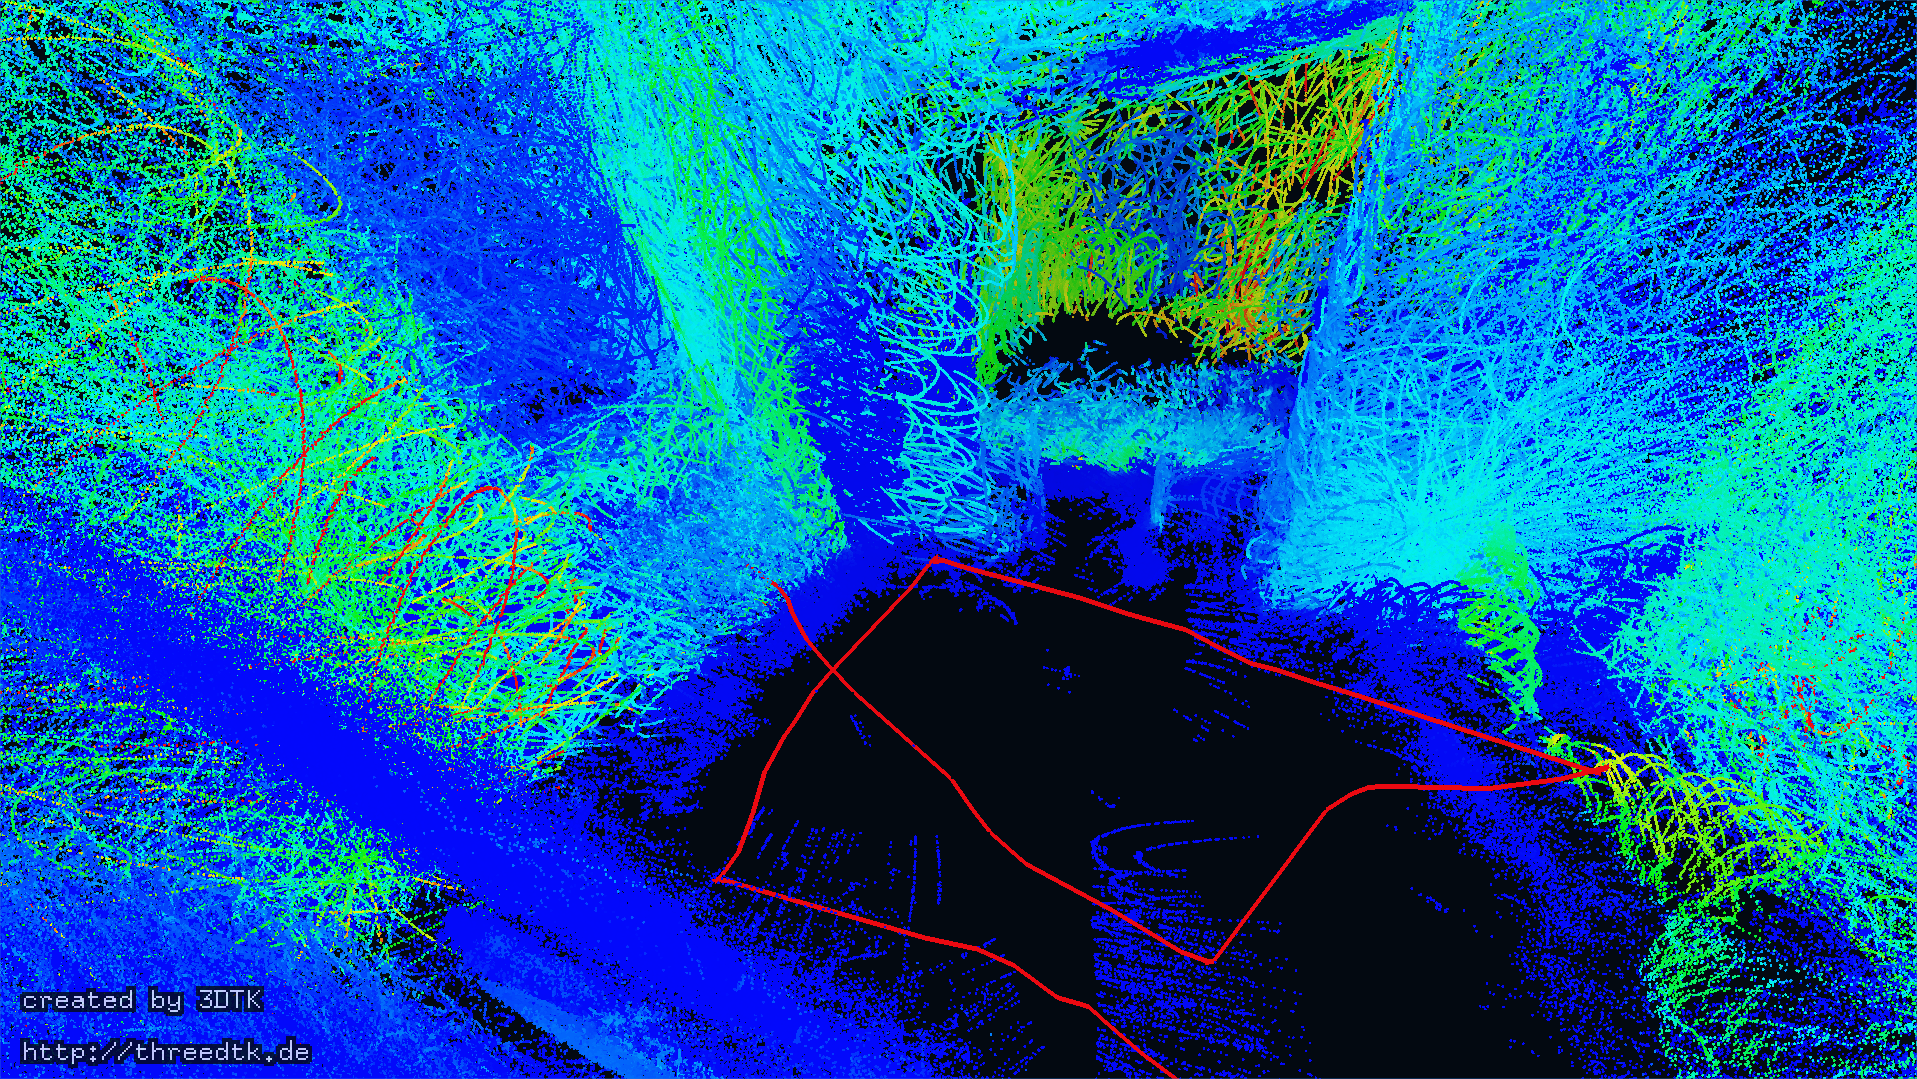
\includegraphics[width=0.495\textwidth]{./images/jasper_uncorr_color}\hfill
	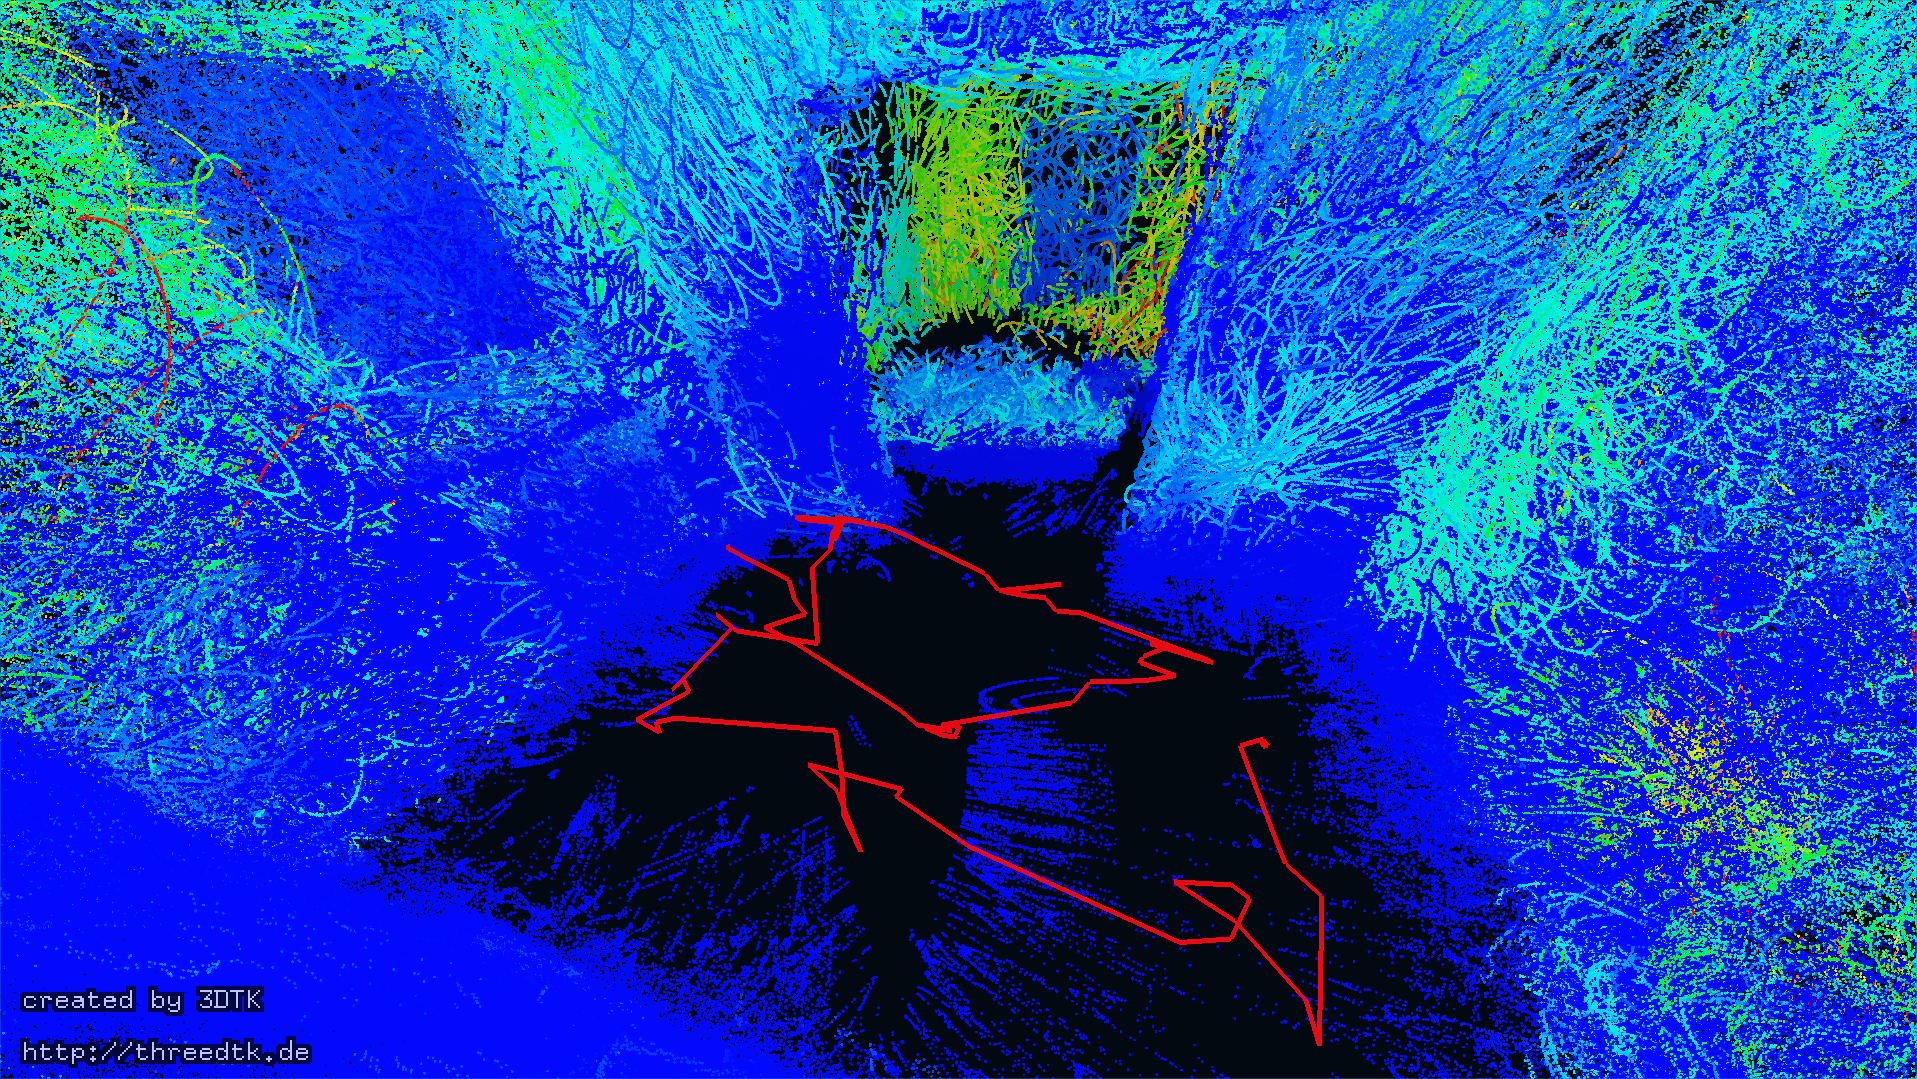
\includegraphics[width=0.495\textwidth]{./images/jasper_corr_color}\\
        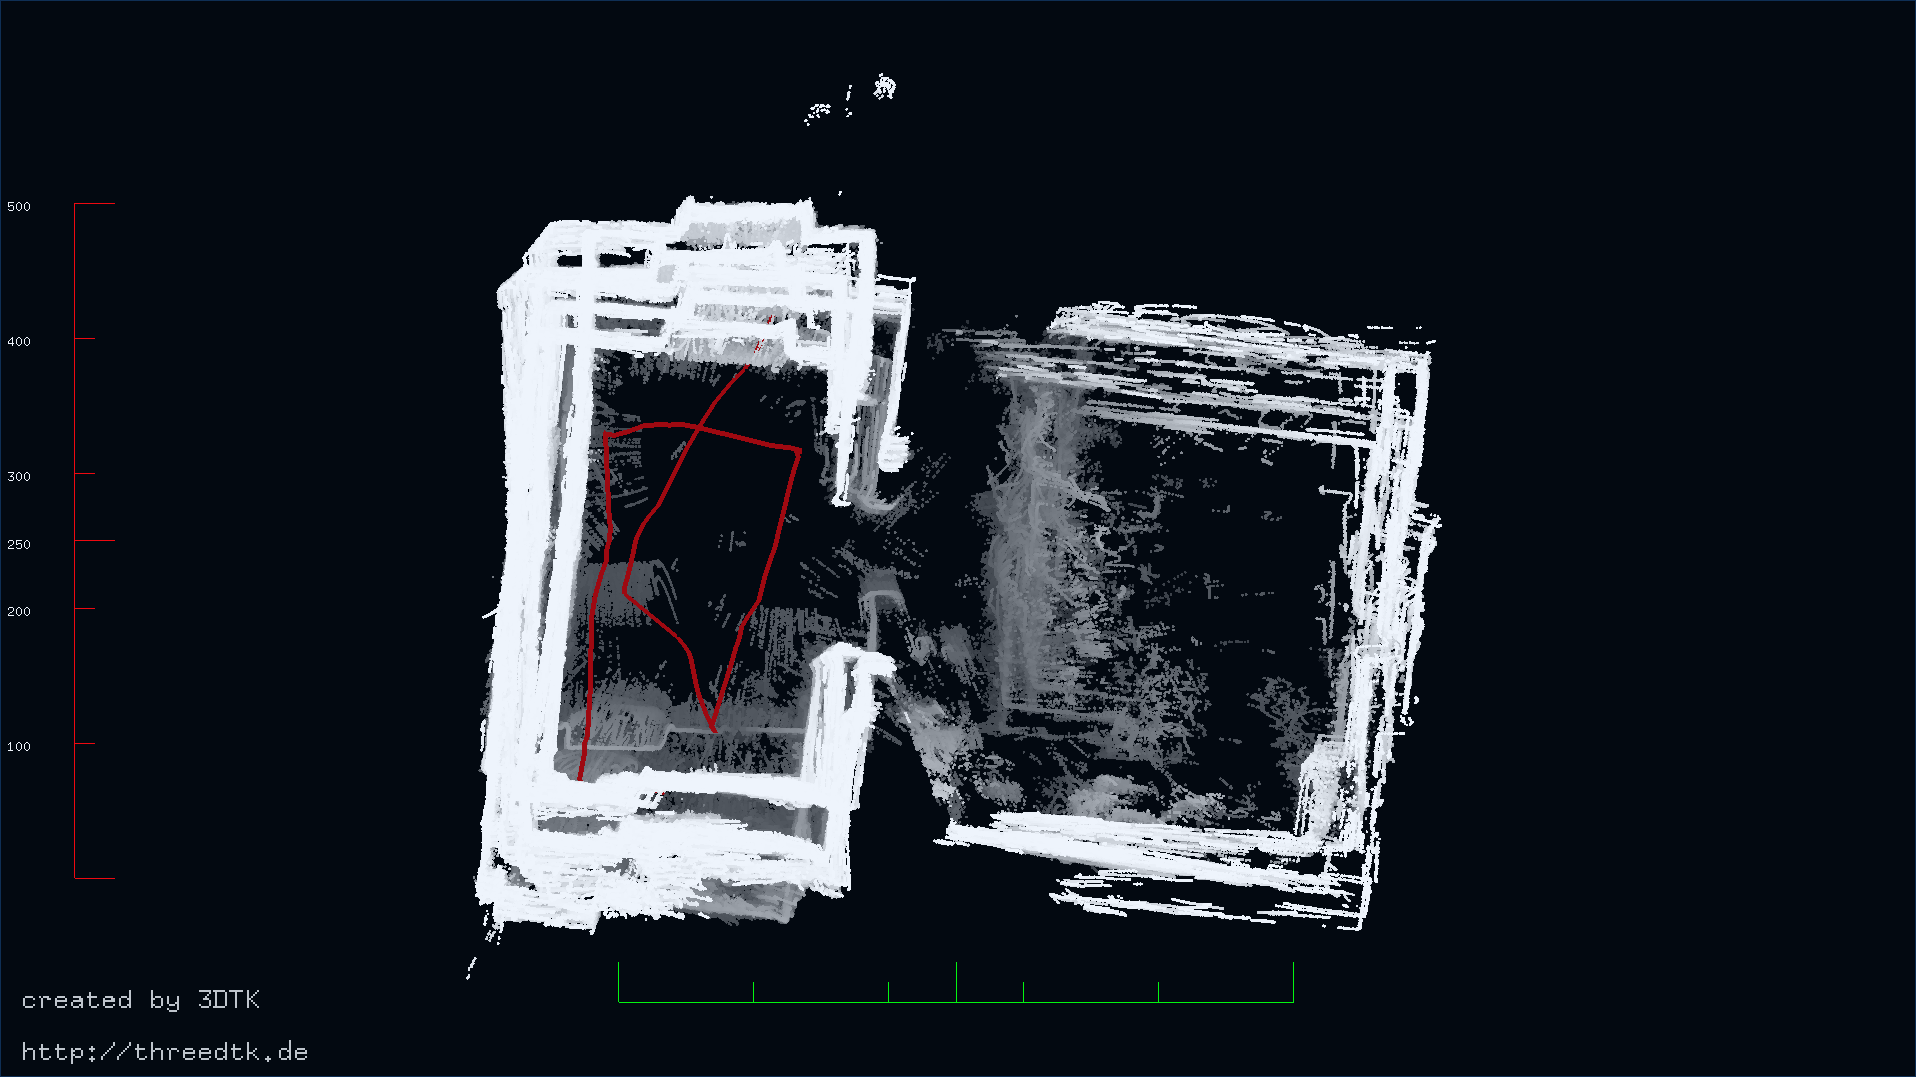
\includegraphics[width=0.495\textwidth]{./images/jasper_uncorr_top}\hfill
        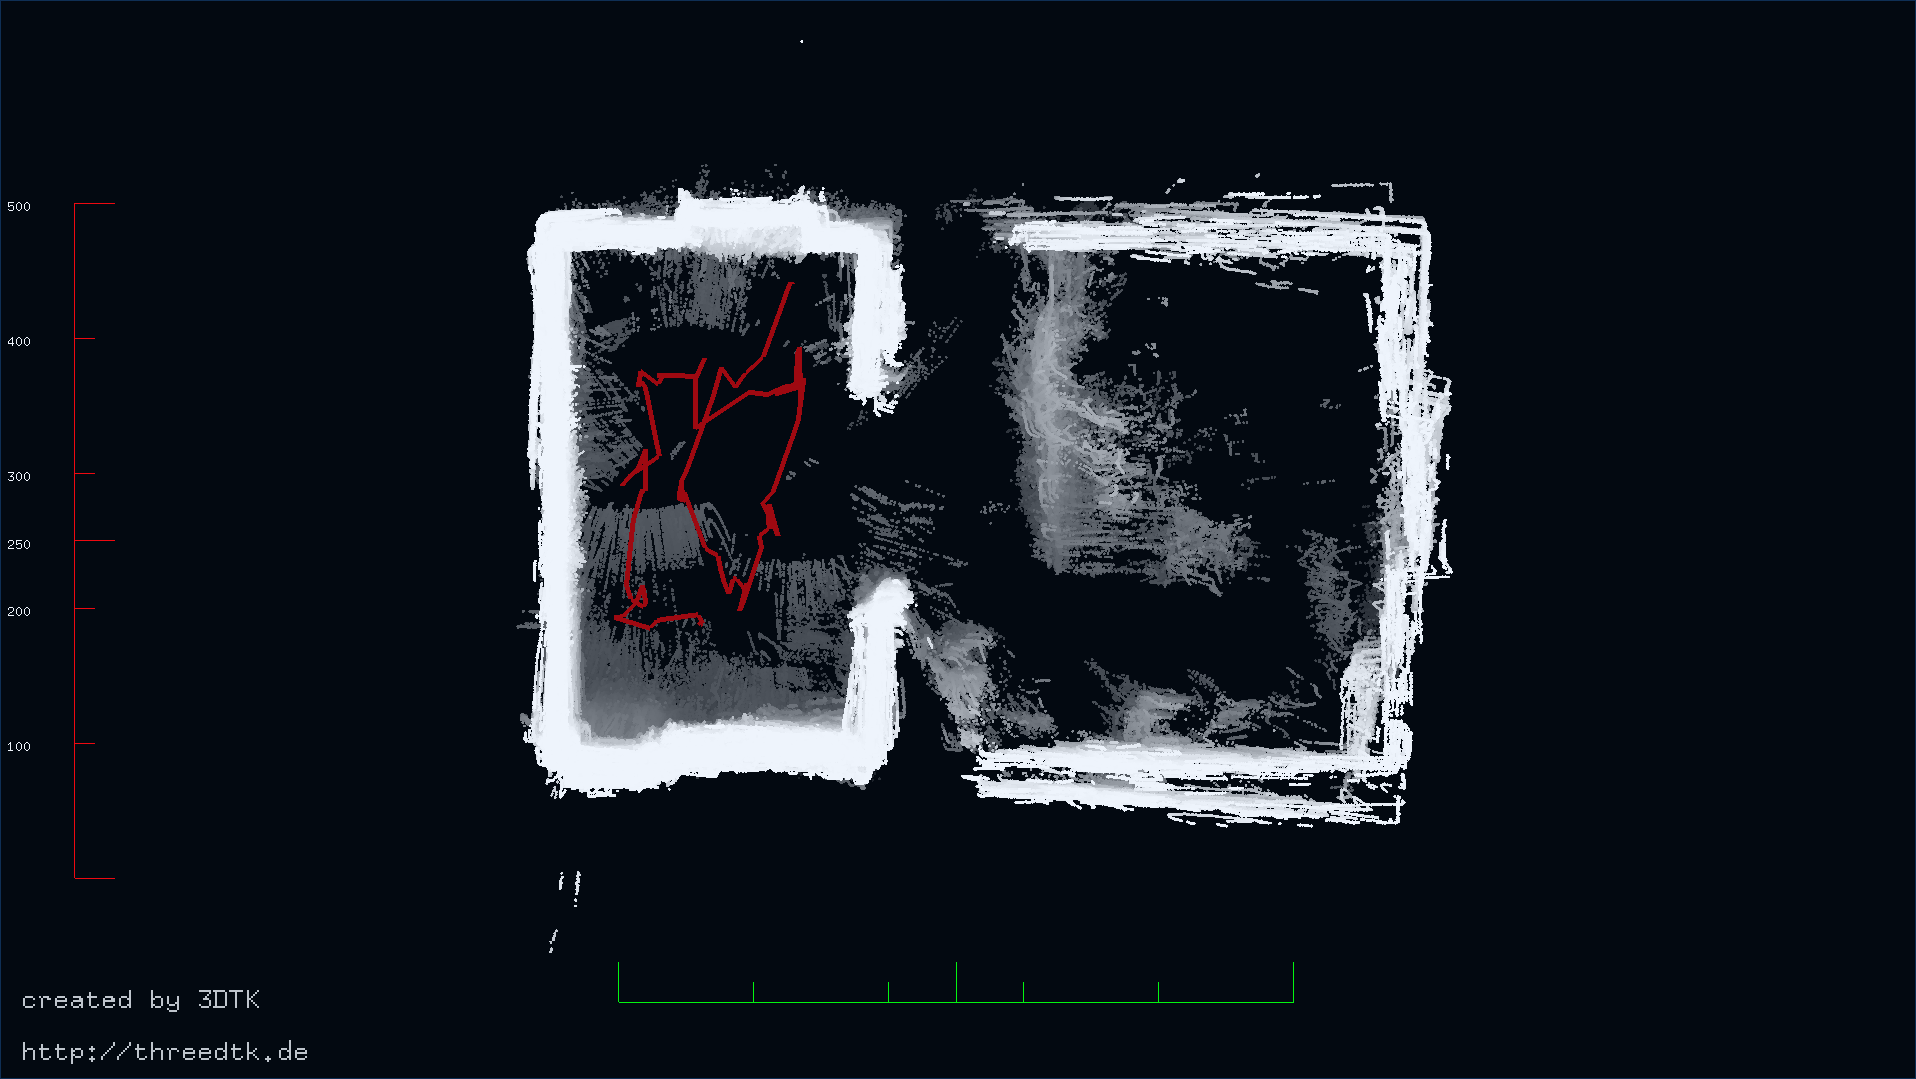
\includegraphics[width=0.495\textwidth]{./images/jasper_corr_top}
        \caption{\DIFaddFL{The point cloud acquired by the rolling sphere before (left) and after (right) applying the plane based registration. View from the interior (top) and a birds-eye view (bottom). Parameters used for optimization: $\epsilon_H = 200$, $\epsilon_P = 300$, $\epsilon_\alpha = \frac{\pi}{4}$, $K = 200$ for AKNN, $d_{growth} = 50$, $N_{c_min} = 800$, $\alpha_0 = [0.001, 0.001, 0.001, 1, 0, 1]^\tau$, $i = 1500$, $k = 1$. An animation of the registration process is given at }\url{https://youtu.be/2J8y7MN10JM}\DIFaddFL{.}}
        \label{fig:jasperhome}
\end{figure*}
\DIFadd{After the registration, the walls of the environment are no longer ambiguous, since all the subsequent scans are matched with the initial plane representation.
When considering the resulting path, it looks distorted.
This is because for some scans, especially empty ones where the sensor points to the ground, no planar features got matched with the global plane model, thus their pose is not optimized.
Improving the path quality is an objective for future works}\DIFaddend .

% This section is commented out
\iffalse
	\subsection{RADLER Results}

	\subsection{Experimental Results REMOVE THIS SECTION}

	For the experimentally acquired datasets a similar procedure is followed. 
	The main difference being, that the scan was pre-registered using a point-to-point based method as described in section~\ref{sec:experimentalSetup}. 
	Here also the point distances to the ground truth (in this case the terrestrially acquired 3D laser scan) is evaluated before and after the plane-based registration process. 

	\begin{figure}
		\centering
		\begin{minipage}[c]{0.25\textwidth}
			\centering	
			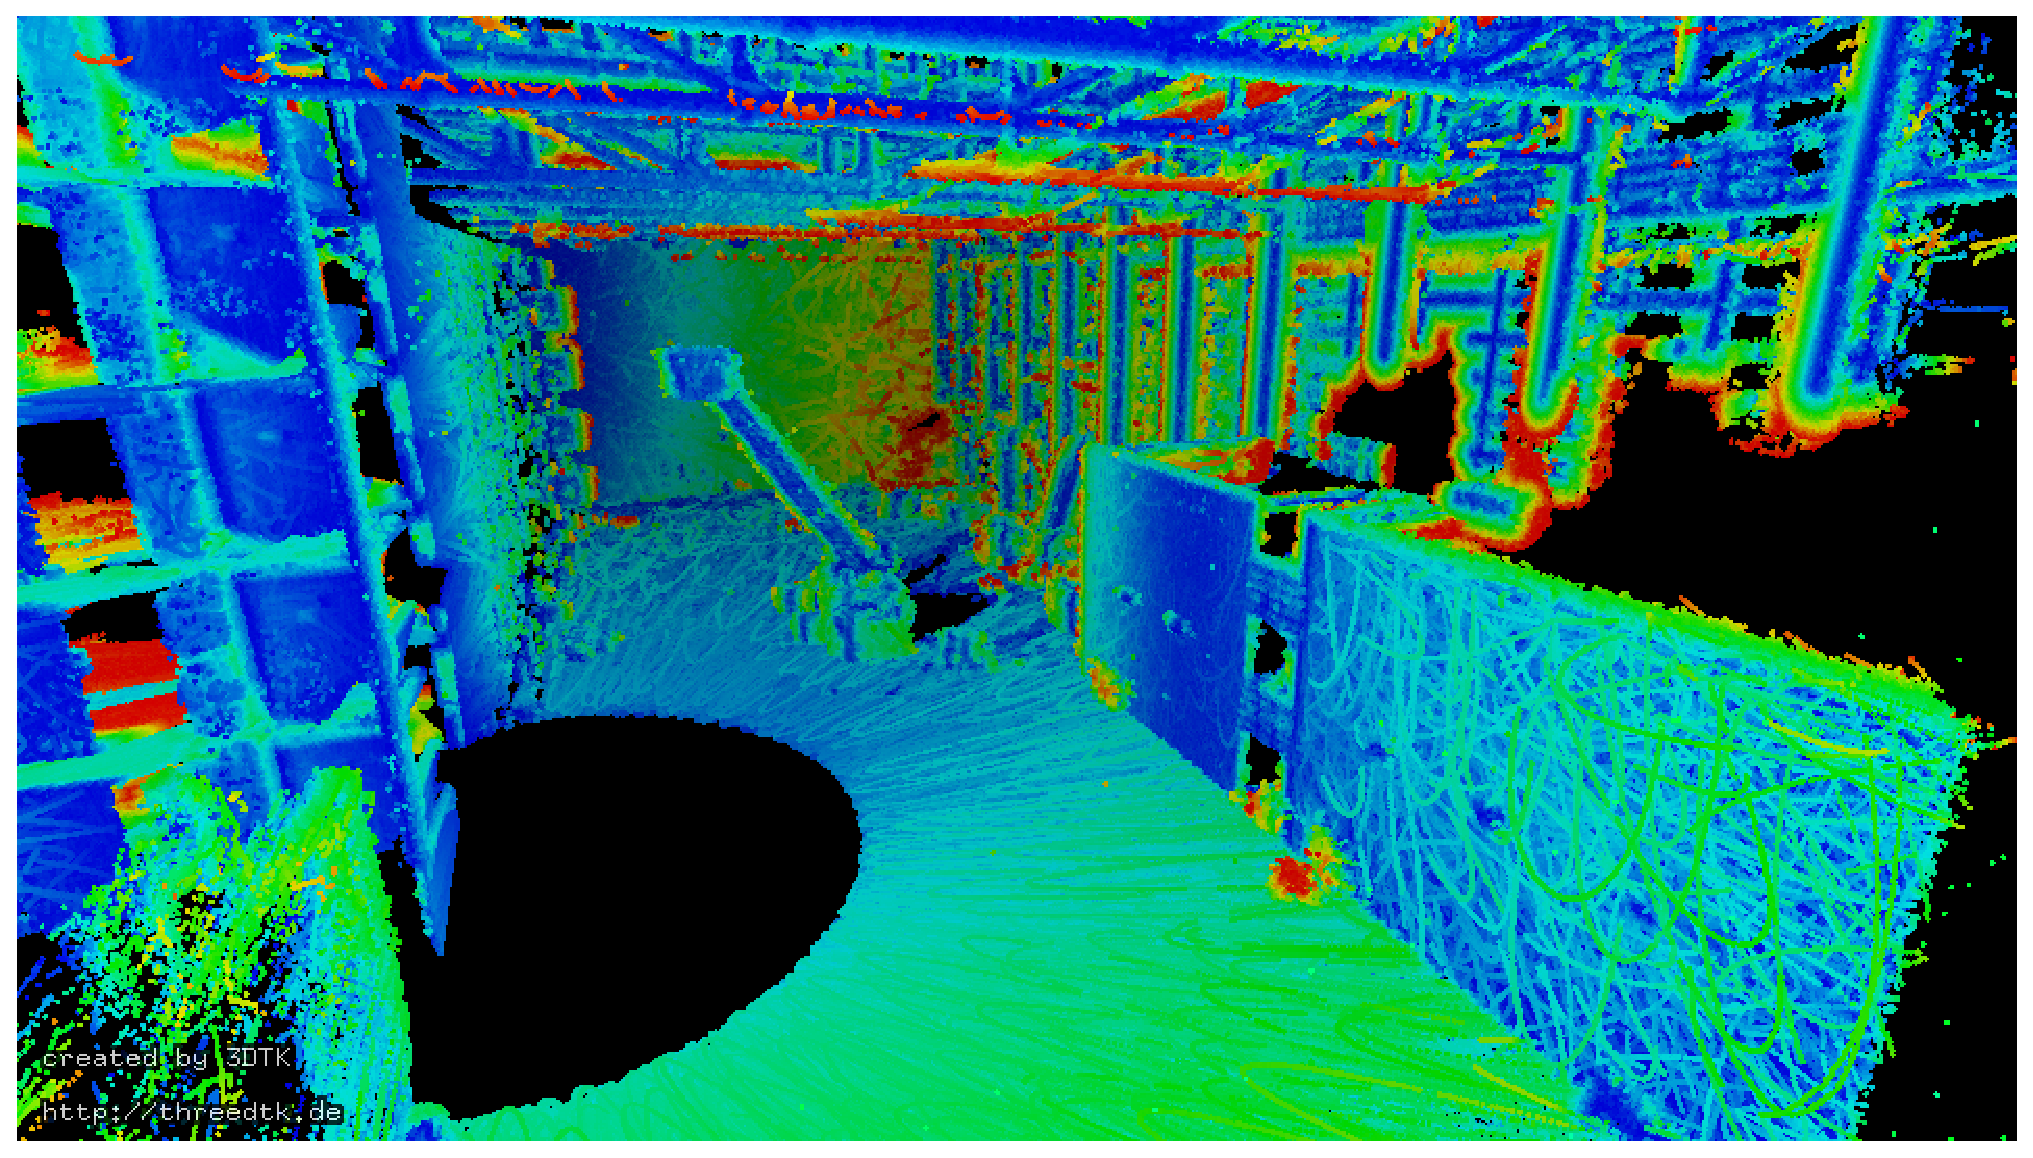
\includegraphics[width = \textwidth]{./images/distances_fire}\\
			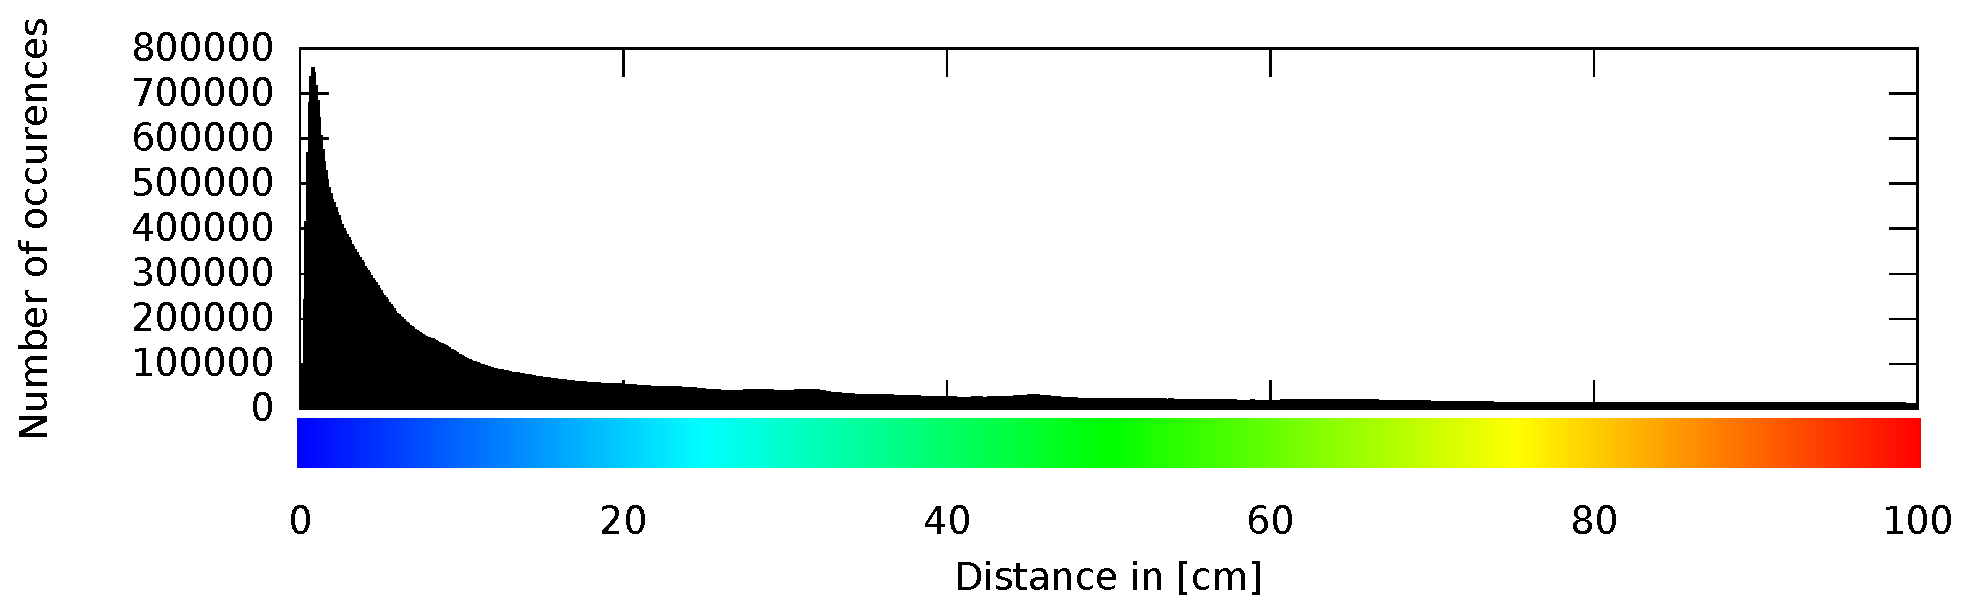
\includegraphics[width = \textwidth]{./images/histogram_fire}
	  	\end{minipage}\hfill
	  	\begin{minipage}[c]{0.25\textwidth}
	  	\end{minipage} 	

		\todo[inline]{Evaluate Plane matching on firefighter school data; histogram after etc}
		\caption{Evaluation of point distances before (left) and after (right) the plane based registration on a experimentally acquired dataset. A maximal distance of \SI{5}{m} is set, such that all points that display a higher distance value are excluded. The left column shows a heat map of distances while the right shows the corresponding histogram. The color mapping is equivalent in both. An animation of the matching process can be seen \href{todo}{here}}
		\label{fig:experimentalEvaluation}
	\end{figure}
\fi

%!TEX root = ../main.tex
\section{Conclusion}

In this paper, we \DIFdelbegin \DIFdel{have proposed a }\DIFdelend \DIFaddbegin \DIFadd{proposed an approach to mobile mapping using a spherical robot. 
Given that a spherical robot inherently rotates for locomotion, we use this movement to also rotate a laser scanner, that consequently measures the robots entire environment.
We propose to post-process the acquire data using a novel }\DIFaddend registration method for man made environments that exploits the structure of those environments. 
\DIFdelbegin \DIFdel{Given that in }\DIFdelend \DIFaddbegin \DIFadd{In }\DIFaddend human-made environments \DIFdelbegin \DIFdel{parallel planes and right angles }\DIFdelend \DIFaddbegin \DIFadd{straight planes }\DIFaddend are abundantly available, \DIFaddbegin \DIFadd{hence }\DIFaddend we employ point-to-plane correspondences to improve a pre-registered 3D point cloud. 
We have evaluated the procedure on a simulated dataset and on \DIFdelbegin \DIFdel{an experimentally acquired dataset with different }\DIFdelend \DIFaddbegin \DIFadd{two experimentally acquired datasets with different laser scanners and }\DIFaddend motion profiles. 
In this evaluation, we have shown that the procedure improves \DIFdelbegin \DIFdel{both }\DIFdelend \DIFaddbegin \DIFadd{all }\DIFaddend datasets and yields maps that better resemble human-made, structures. 
In particular, the qualitative structure of the environments is reconstructed well. 
In the resulting maps, the parallel walls are clearly improved.
\DIFdelbegin %DIFDELCMD < 

%DIFDELCMD < %%%
\DIFdel{However, as section~\ref{sec:experimentalSetup} shows, some outliers remain in the registered point cloud due to the simplistic point-to-plane correspondence model.
This to be improved in future studies.
One idea to do so is to employ a local clustering technique onto the individual scans before registering them globally. 
Points from the scan with a similar normal get clustered together if their distance is small enough.
This way, a cluster represents a local plane while at the same time storing all the points that belong to that plane.
Point-to-plane correspondences then arise from the intersection of local clusters with global planes}\DIFdelend \DIFaddbegin \DIFadd{The simulation results show that the algorithm has the potential to improve the map quality based on point-distances by approximately a factor of ten}\DIFaddend .

\DIFdelbegin \DIFdel{Needless to say, a lot of work remains to be done. 
}\DIFdelend %
Right now, not all steps in the procedure are autonomous, in particular the parameter tuning. 
In the future, one goal is to increase the autonomy of the system.
One approach is to introduce soft-locks for the optimization dimensions.
I.e., instead of locking some dimensions entirely from being used for optimization, they are weighted based on the dynamics of the system that encode which noise source is more likely.  
\DIFaddbegin 

\DIFaddend %
\DIFdelbegin \DIFdel{Currently, we are assembling the sphere of Figure~\ref{fig:robotRender} to test it in real environments.
Unfortunately, this sphere will be too large to fit our floating setup, thus it will be tested in an office like environment.
Furthermore, }\DIFdelend \DIFaddbegin \DIFadd{The biggest issue with the presented algorithm currently is that the global plane model is established only once at initialization, but never updated afterwards.
Utilizing the local planar clustering (LPC) of the individual line scans for updating the global plane model step by step is currently the primary objective of future studies.
One idea is to calculate the convex hulls of the LPC, and combine them with the global planes sequentially.
Therefore, we expect to increase robustness and autonomy of the registration procedure.
}

%DIF > 
\DIFadd{Furthermore, more experimental evaluation is required, hence }\DIFaddend we will test our rolling and scanning spheres on a rail system to achieve repeatable trajectories. 

%!TEX root = ../main.tex
\section*{Acknowledgement}

The authors thank the Cylon team (Ignacio Dorado Llamas, Timothy Randolph, Camilo Andres Reyes Mantilla) for designing and building the prototype and Timo Burger for acquiring the floating table data set.
Special thanks to Dieter Ziegler and Sergio Montenegro for supporting our work.
We acknowledge funding from the ESA Contract No. 4000130925/20/NL/GLC for the study ``DAEDALUS -- Descent And Exploration in Deep Autonomy of Lava Underground Structures'' within the Open Space Innovation Platform (OSIP) lunar caves-system and the Elite Network Bavaria (ENB) for providing funds for the academic program ``Satellite Technology''.


\begin{thebibliography}{10}
\expandafter\ifx\csname url\endcsname\relax
  \def\url#1{\texttt{#1}}\fi
\expandafter\ifx\csname urlprefix\endcsname\relax\def\urlprefix{URL }\fi
\expandafter\ifx\csname href\endcsname\relax
  \def\href#1#2{#2} \def\path#1{#1}\fi

\bibitem{Bosse2012-zebedee}
M.~Bosse, R.~Zlot, P.~Flick, Zebedee: Design of a spring-mounted 3-d range
  sensor with application to mobile mapping, IEEE Transactions on Robotics
  28~(5) (2012) 1104--1119.
\newblock \href {http://dx.doi.org/10.1109/TRO.2012.2200990}
  {\path{doi:10.1109/TRO.2012.2200990}}.

\bibitem{JPRS2016}
V.~V. Lehtola, J.-P. Virtanen, M.~T. Vaaja, H.~Hyypp{\"a}, A.~N{\"u}chter,
  \href{https://robotik.informatik.uni-wuerzburg.de/telematics/download/jprs2016.pdf}{{Localization
  of a Mobile Laser Scanner via Dimensional Reduction}}, ISPRS Journal of
  Photogrammetry and Remote Sensing (JPRS) 121 (2016) 48--59.
\newblock \href {http://dx.doi.org/10.1016/j.isprsjprs.2016.09.004}
  {\path{doi:10.1016/j.isprsjprs.2016.09.004}}.
\newline\urlprefix\url{https://robotik.informatik.uni-wuerzburg.de/telematics/download/jprs2016.pdf}

\bibitem{Borrmann2020-RADLER}
D.~Borrmann, S.~Jörissen, A.~Nuchter, {RADLER -- A RADial LasER scanning
  device}, in: {Proceedings of the International Symposium on Experimental
  Research}, {Buenos Aires, Argentina}, 2020, pp. 655--664.
\newblock \href {http://dx.doi.org/10.1007/978-3-030-33950-0_56}
  {\path{doi:10.1007/978-3-030-33950-0_56}}.

\bibitem{LauterbackEtAl2015-Backpack}
H.~A. Lauterbach, D.~Borrmann, R.~Heß, D.~Eck, K.~Schilling, A.~Nüchter,
  \href{https://www.mdpi.com/2072-4292/7/10/13753}{Evaluation of a
  backpack-mounted 3d mobile scanning system}, Remote Sensing 7~(10) (2015)
  13753--13781.
\newblock \href {http://dx.doi.org/10.3390/rs71013753}
  {\path{doi:10.3390/rs71013753}}.
\newline\urlprefix\url{https://www.mdpi.com/2072-4292/7/10/13753}

\bibitem{WWWLeicaBackpack}
Leica, Leica pegasus:backpack,
  {\small{\url{www.leica-geosystems.com/de/Leica-PegasusBackpack_106730.htm}}}
  ({May} {2015}).

\bibitem{SpotRobot}
{Boston Dynamics}, Spot robot, \url{https://www.bostondynamics.com/spot}
  (2021).

\bibitem{Fankhauser2018-ANYmal}
P.~Fankhauser, M.~Bloesch, M.~Hutter, Probabilistic terrain mapping for mobile
  robots with uncertain localization, IEEE Robotics and Automation Letters
  3~(4) (2018) 3019--3026.
\newblock \href {http://dx.doi.org/10.1109/LRA.2018.2849506}
  {\path{doi:10.1109/LRA.2018.2849506}}.

\bibitem{RossiMaurelliUnnithanetal.2021}
A.~P. Rossi, F.~Maurelli, V.~Unnithan, H.~Dreger, K.~Mathewos, N.~Pradhan,
  D.-A. Corbeanu, R.~Pozzobon, M.~Massironi, S.~Ferrari, C.~Pernechele,
  L.~Paoletti, E.~Simioni, P.~Maurizio, T.~Santagata, D.~Borrmann,
  A.~N{\"u}chter, A.~Bredenbeck, J.~Zevering, F.~Arzberger, C.~A.~R. Mantilla,
  Daedalus - descent and exploration in deep autonomy of lava underground
  structures, Tech. Rep.~21, Institut f{\"u}r Informatik (2021).
\newblock \href {http://dx.doi.org/10.25972/OPUS-22791}
  {\path{doi:10.25972/OPUS-22791}}.

\bibitem{9233654}
J.~Guo, X.~Chen, S.~Guo, J.~Xu, Study on map construction of spherical robot
  based on statistical filtering, in: 2020 IEEE International Conference on
  Mechatronics and Automation (ICMA), 2020, pp. 1269--1274.
\newblock \href {http://dx.doi.org/10.1109/ICMA49215.2020.9233654}
  {\path{doi:10.1109/ICMA49215.2020.9233654}}.

\bibitem{JFR2006}
A.~N{\"u}chter, K.~Lingemann, J.~Hertzberg, H.~Surmann,
  \href{https://robotik.informatik.uni-wuerzburg.de/telematics/download/jfr2007.pdf}{{6D
  SLAM -- 3D Mapping Outdoor Environments}}, Journal of Field Robotics (JFR),
  Special Issue on Quantitative Performance Evaluation of Robotic and
  Intelligent Systems 24~(8--9) (2007) 699--722.
\newblock \href {http://dx.doi.org/10.1002/rob.20209}
  {\path{doi:10.1002/rob.20209}}.
\newline\urlprefix\url{https://robotik.informatik.uni-wuerzburg.de/telematics/download/jfr2007.pdf}

\bibitem{RAS2007}
D.~Borrmann, J.~Elseberg, K.~Lingemann, A.~N{\"u}chter, J.~Hertzberg,
  \href{https://robotik.informatik.uni-wuerzburg.de/telematics/download/ras2007.pdf}{Globally
  consistent 3d mapping with scan matching}, Journal Robotics and Autonomous
  Systems (JRAS) 56~(2) (2008) 130--142.
\newblock \href {http://dx.doi.org/10.1016/j.robot.2007.07.002}
  {\path{doi:10.1016/j.robot.2007.07.002}}.
\newline\urlprefix\url{https://robotik.informatik.uni-wuerzburg.de/telematics/download/ras2007.pdf}

\bibitem{Zhang2014}
J.~Zhang, S.~Singh, Loam: Lidar odometry and mapping in real-time, in:
  Robotics: Science and Systems Conference (RSS), 2014.
\newblock \href {http://dx.doi.org/10.15607/RSS.2014.X.007}
  {\path{doi:10.15607/RSS.2014.X.007}}.

\bibitem{Droeschel2018}
D.~Droeschel, S.~Behnke,
  \href{http://dx.doi.org/10.1109/ICRA.2018.8461000}{Efficient continuous-time
  slam for 3d lidar-based online mapping}, 2018 IEEE International Conference
  on Robotics and Automation (ICRA)\href
  {http://dx.doi.org/10.1109/icra.2018.8461000}
  {\path{doi:10.1109/icra.2018.8461000}}.
\newline\urlprefix\url{http://dx.doi.org/10.1109/ICRA.2018.8461000}

\DIFaddbegin \bibitem{navvis}
\DIFadd{NavVis, The navvis vlx mobile mapping system, }\url{https://www.navvis.com}\DIFadd{,
  accessed on 05.07.2021.
}

\DIFaddend \bibitem{Besl1992}
P.~J. {Besl}, N.~D. {McKay}, A method for registration of 3-d shapes, IEEE
  Transactions on Pattern Analysis and Machine Intelligence 14~(2) (1992)
  239--256.
\newblock \href {http://dx.doi.org/10.1109/34.121791}
  {\path{doi:10.1109/34.121791}}.

\bibitem{Pathak:2010}
K.~Pathak, A.~Birk, N.~Vaskevicius, J.~Poppinga, Fast registration based on
  noisy planeswith unknown correspondences for 3d mapping, IEEE Transactions on
  Robotics 26~(3) (2010) 424--441.
\newblock \href {http://dx.doi.org/10.1109/TRO.2010.2042989}
  {\path{doi:10.1109/TRO.2010.2042989}}.

\bibitem{Foerstner2017}
W.~{Förstner}, K.~{Khoshelham}, Efficient and accurate registration of point
  clouds with plane to plane correspondences, in: 2017 IEEE International
  Conference on Computer Vision Workshops (ICCVW), 2017, pp. 2165--2173.
\newblock \href {http://dx.doi.org/10.1109/ICCVW.2017.253}
  {\path{doi:10.1109/ICCVW.2017.253}}.

\bibitem{favre2021}
K.~Favre, M.~Pressigout, E.~Marchand, L.~Morin,
  \href{https://hal.archives-ouvertes.fr/hal-03108891}{{A Plane-based Approach
  for Indoor Point Clouds Registration}}, in: {ICPR 2020 - 25th International
  Conference on Pattern Recognition}, Milan (Virtual), Italy, 2021.
\newline\urlprefix\url{https://hal.archives-ouvertes.fr/hal-03108891}

\DIFaddbegin \bibitem{Lin_2020}
\DIFadd{J.~Lin, F.~Zhang, }{\DIFadd{Loam livox: A fast, robust, high-precision LiDAR odometry
  and mapping package for LiDARs of small FoV}}\DIFadd{, in: proceedings of the IEEE
  International Conference on Robotics and Automation (ICRA), 2020, pp.
  3126--3131.
}\newblock \href {\DIFadd{http://dx.doi.org/10.1109/ICRA40945.2020.9197440}}
  {\path{doi:10.1109/ICRA40945.2020.9197440}}\DIFadd{.
}

\bibitem{Zhou_2021}
\DIFadd{L.~Zhou, S.~Wang, M.~Kaess, }{\DIFadd{$\pi$}}\DIFadd{-}{\DIFadd{LSAM}}\DIFadd{: }{\DIFadd{LiDAR}} \DIFadd{smoothing and mapping with
  planes, in: Proceedings of IEEE International Conference on Robotics and
  Automation (ICRA '21), Xi'an, China, 2021, to appear.
}

\bibitem{Jung_2015}
\DIFadd{J.~Jung, S.~Yoon, S.~Ju, J.~Heo, }{\DIFadd{Development of kinematic 3D laser scanning
  system for indoor mapping and as-built BIM using constrained SLAM}}\DIFadd{, Sensors
  15~(10) (2015) 26430--26456.
}\newblock \href {\DIFadd{http://dx.doi.org/10.3390/s151026430}}
  {\path{doi:10.3390/s151026430}}\DIFadd{.
}

\bibitem{Grant_2018}
\DIFadd{W.~S. Grant, R.~C. Voorhies, L.~Itti, }{\DIFadd{Efficient Velodyne SLAM with point and
  plane features}}\DIFadd{, Autonomous Robots 43 (2019) 1207--1224.
}\newblock \href {\DIFadd{http://dx.doi.org/10.1007/s10514-018-9794-6}}
  {\path{doi:10.1007/s10514-018-9794-6}}\DIFadd{.
}

\bibitem{Geneva_2018}
\DIFadd{P.~Geneva, K.~Eckenhoff, Y.~Yang, G.~Huang, }{\DIFadd{LIPS: LiDAR-Inertial 3D Plane
  SLAM}}\DIFadd{, in: Proceedings of the IEEE/RSJ International Conference on
  Intelligent Robots and Systems (IROS '18), 2018, pp. 123--130.
}\newblock \href {\DIFadd{http://dx.doi.org/10.1109/IROS.2018.8594463}}
  {\path{doi:10.1109/IROS.2018.8594463}}\DIFadd{.
}

\bibitem{wei2021groundslam}
\DIFadd{X.~Wei, J.~Lv, J.~Sun, S.~Pu, }{\DIFadd{Ground-SLAM: Ground Constrained LiDAR SLAM for
  Structured Multi-Floor Environments}} \DIFadd{(2021).
}\newblock \href {\DIFadd{http://arxiv.org/abs/2103.03713}} {\path{arXiv:2103.03713}}\DIFadd{.
}

\DIFaddend \bibitem{Borrmann2010}
J.~Elseberg, D.~Borrmann, K.~Lingemann, A.~Nüchter, Non-rigid registration and
  rectification of 3d laser scans, in: 2010 IEEE/RSJ International Conference
  on Intelligent Robots and Systems, 2010, pp. 1546--1552.
\newblock \href {http://dx.doi.org/10.1109/IROS.2010.5652278}
  {\path{doi:10.1109/IROS.2010.5652278}}.

\DIFaddbegin \bibitem{Stoyanov2009}
\DIFadd{T.~Stoyanov, A.~J. Lilienthal, Maximum likelihood point cloud acquisition from
  a mobile platform, in: 2009 International Conference on Advanced Robotics
  (ICAR), 2009, pp. 1--6.
}

\bibitem{Bosse2009}
\DIFadd{M.~Bosse, R.~Zlot, Continuous 3d scan-matching with a spinning 2d laser, in:
  2009 IEEE International Conference on Robotics and Automation, 2009, pp.
  4312--4319.
}\newblock \href {\DIFadd{http://dx.doi.org/10.1109/ROBOT.2009.5152851}}
  {\path{doi:10.1109/ROBOT.2009.5152851}}\DIFadd{.
}

\DIFaddend \bibitem{REMSEN2013}
J.~Elseberg, D.~Borrmann, A.~N{\"u}chter,
  \href{https://robotik.informatik.uni-wuerzburg.de/telematics/download/remotesensing2013.pdf}{{Algorithmic
  solutions for computing accurate maximum likelihood 3D point clouds from
  mobile laser scanning platforms}}, Remote Sensing 5~(11) (2013) 5871--5906.
\newblock \href {http://dx.doi.org/10.3390/rs5115871}
  {\path{doi:10.3390/rs5115871}}.
\newline\urlprefix\url{https://robotik.informatik.uni-wuerzburg.de/telematics/download/remotesensing2013.pdf}

\bibitem{3DRESEARCH2011}
D.~Borrmann, J.~Elseberg, A.~N{\"u}chter, K.~Lingemann,
  \href{https://robotik.informatik.uni-wuerzburg.de/telematics/download/3dresearch2011.pdf}{{The
  3D Hough Transform for Plane Detection in Point Clouds -- A Review and A new
  Accumulator Design}}, Journal of 3D Research 2~(2) (2011) 1--13.
\newblock \href {http://dx.doi.org/10.1007/3DRes.02(2011)3}
  {\path{doi:10.1007/3DRes.02(2011)3}}.
\newline\urlprefix\url{https://robotik.informatik.uni-wuerzburg.de/telematics/download/3dresearch2011.pdf}

\DIFaddbegin \bibitem{Honti2018}
\DIFadd{R.~Honti, J.~Erdélyi, A.~Kopacik, Plane segmentation from point clouds,
  Pollack Periodica 13 (2018) 159--171.
}\newblock \href {\DIFadd{http://dx.doi.org/10.1556/606.2018.13.2.16}}
  {\path{doi:10.1556/606.2018.13.2.16}}\DIFadd{.
}

\bibitem{Gaspers2011}
\DIFadd{B.~Gaspers, J.~Stückler, J.~Welle, D.~Schulz, S.~Behnke, Efficient
  multi-resolution plane segmentation of 3d point clouds, 2011, pp. 145--156.
}\newblock \href {\DIFadd{http://dx.doi.org/10.1007/978-3-642-25489-5_15}}
  {\path{doi:10.1007/978-3-642-25489-5_15}}\DIFadd{.
}

\bibitem{Engelmann2018}
\DIFadd{F.~Engelmann, T.~Kontogianni, J.~Schult, B.~Leibe,
  }\href{http://arxiv.org/abs/1810.01151}{Know what your neighbors do: 3d
  semantic segmentation of point clouds}\DIFadd{, CoRR abs/1810.01151.
}\newblock \href {\DIFadd{http://arxiv.org/abs/1810.01151}} {\path{arXiv:1810.01151}}\DIFadd{.
}\newline\urlprefix\url{http://arxiv.org/abs/1810.01151}

\bibitem{pga}
\DIFadd{D.~Sunday, }{\DIFadd{Practical Geometry Algorithms}}\DIFadd{, Independently published, 2021.
}

\bibitem{aknnbbs}
\DIFadd{J.~S. Beis, D.~G. Lowe, Shape indexing using approximate nearest-neighbour
  search in high-dimensional spaces, CVPR '97, IEEE Computer Society, 1997.
}\newblock \href {\DIFadd{http://dx.doi.org/10.1109/CVPR.1997.609451}}
  {\path{doi:10.1109/CVPR.1997.609451}}\DIFadd{.
}

\DIFaddend \bibitem{diebel2006representing}
J.~Diebel, Representing attitude: Euler angles, unit quaternions, and rotation
  vectors, Matrix 58~(15-16) (2006) 1--35.

\bibitem{zeiler2012adadelta}
M.~D. Zeiler, Adadelta: An adaptive learning rate method (2012).
\newblock \href {http://arxiv.org/abs/1212.5701} {\path{arXiv:1212.5701}}.

\bibitem{LivoxMid40-100}
Livox, {Livox Mid40 and Mid100},
  \url{https://www.livoxtech.com/mid-40-and-mid-100} (2021).

\bibitem{thorlabs}
ThorLabs, Application note risley prism scanner,
  \url{https://www.thorlabs.com/images/tabimages/Risley_Prism_Scanner_App_Note.pdf}\DIFaddbegin \DIFadd{.
}

\bibitem{PhidgetSpatial}
\DIFadd{Phidget, }{\DIFadd{PhidgetSpatial Precision 3/3/3}}\DIFadd{,
  }\url{https://www.phidgets.com/?&prodid=32} \DIFadd{(2021)}\DIFaddend .

\bibitem{madgwick2010efficient}
S.~Madgwick, An efficient orientation filter for inertial and inertial/magnetic
  sensor arrays, Report x-io and University of Bristol (UK) 25 (2010) 113--118.

\end{thebibliography}


\end{document}
